% Author Alfredo Sánchez Alberca (asalber@ceu.es)

\documentclass[a4paper,titlepage]{article}
%===============================================
\usepackage[english]{babel}
\usepackage[top=3cm, bottom=3cm, left=2.54cm, right=2.54cm, marginparwidth=2mm]{geometry}

% COLORS
\usepackage[table]{xcolor} 
\definecolor{color1}{RGB}{5,161,230}
\definecolor{color2}{RGB}{238,50,36}
\definecolor{ocre}{RGB}{243,102,25} % Define the orange color used for highlighting throughout the book
\definecolor{blueceu}{RGB}{5,161,230} % Blue color of CEU logo
\definecolor{greenceu}{RGB}{185,209,16} % Green color of CEU logo
\definecolor{redceu}{RGB}{238,50,36} % Red color of CEU logo
\definecolor{grayceu}{RGB}{111,107,83} % Gray color of CEU logo
\definecolor{coral}{rgb}{1,0.5,0.31} % Orange color for graphics
\definecolor{royalblue1}{rgb}{0.28,0.46,1} % Blue color for graphics
\definecolor{mygreen}{rgb}{0,0.8,0} % Green color for graphics
\definecolor{chaptergrey}{RGB}{5,161,230} % Blue color of CEU logo

% MATH
\usepackage{amsmath}
\usepackage{amssymb}
\usepackage{amsthm}

% GRAPHICS
\usepackage{graphicx}
\usepackage{pgfplots}
\usepackage{tikz}
\usetikzlibrary{external,arrows,arrows.meta,calc,shapes,shapes.arrows,positioning,snakes,decorations.pathreplacing}
\usepackage{tkz-euclide}
\usetkzobj{all}

\usepackage{multicol}
\usepackage[inline]{enumitem}
\usepackage{fancyhdr}
\pagestyle{fancy}
\lhead{\textsc{\textcolor{blueceu}{CEU San Pablo University}}}
\rhead{\textsl{\textsf{\textcolor{blueceu}{Department of Applied Math and Statistics}}}}
\renewcommand{\headrulewidth}{0pt}

\usepackage{booktabs}


% SOLUTIONS
\newif\ifsolution
% \solutiontrue  % Comment to hide solutions

\newtheoremstyle{solution} % Theorem style name
{-5pt} % Space above
{7pt} % Space below
{\normalfont} % Body font
{-28pt} % Indent amount
{\bf} % Theorem head font
{\kern-11.5pt} % Punctuation after theorem head
{19pt} % Space after theorem head
{\begin{tikzpicture}
\draw (0,0) node [fill=color2, xshift=4mm, inner
sep=2pt]{\includegraphics[scale=0.3]{img/bulb}};
\end{tikzpicture}}

\theoremstyle{solution}
\newtheorem{solutionT}{Solution}

\RequirePackage[framemethod=default]{mdframed}

% Solution box
\newmdenv[skipabove=7pt,
skipbelow=10pt,
rightline=false,
leftline=true,
topline=false,
bottomline=false,
linecolor=color2,
backgroundcolor=black!5,
innerleftmargin=5pt,
innerrightmargin=5pt,
innertopmargin=4pt,
innerbottommargin=5pt,
leftmargin=0pt,
rightmargin=0pt,
linewidth=4pt]{solBox}		

\usepackage{comment}
\ifsolution
  \newenvironment{sol}{\ifsolution\begin{solBox}\begin{solutionT}}{\end{solutionT}\end{solBox}\fi}
\else
  \excludecomment{sol}
\fi

% PDF
\usepackage[colorlinks=true]{hyperref}
\hypersetup{pdfauthor={Alfredo Sánchez Alberca (asalber@ceu.es)}, pdftitle={Ejercicios de Estad\'istica} } 
\usepackage{url}

\renewcommand{\floatpagefraction}{.8}
\renewcommand{\textfraction}{.1}


\begin{document}
\sloppy

\title{\vskip 2cm
\Huge \textbf{\textsf{\quad \textcolor{blueceu}{EXERCISES OF STATISTICS}\quad}}\\
   \vskip 1cm
\Large \sffamily
\begin{tabular}{rl}
\textcolor{blueceu}{Subject:} & Statistics Applied tho the Health Sciences\\
\textcolor{blueceu}{Course:} & $2^{nd}$\\
\textcolor{blueceu}{Degree:} &  Physiotherapy\\
\textcolor{blueceu}{Year:} & 2015-2016\\
\textcolor{blueceu}{Authors:} & Santiago Angulo D\'iaz-Parre\~no (\url{sangulo@ceu.es})\\
& Jos\'e Miguel C\'ardenas Rebollo (\url{cardenas@ceu.es})\\
& Anselmo Romero Lim\'on (\url{arlimon@ceu.es})\\
& Alfredo S\'anchez Alberca (\url{asalber@ceu.es})
\end{tabular}
}

\author{}
\date{\includegraphics[scale=0.3]{img/logo_uspceu}}

\maketitle
\newpage
\tableofcontents
\newpage

% Author Alfredo Sánchez Alberca (asalber@ceu.es)

\newproblem*{des-1a}{far}{}
%STATEMENT
{A survey about the daily number of medicines consumed by people over 70 years, shows the following results:

\begin{center}
3\quad 1\quad 2\quad 2\quad 0\quad 1\quad 4\quad 2\quad 3\quad 5\quad 1\quad 3\quad 2\quad 3\quad 1\quad 4\quad 2\quad 4\quad 3\quad 2 \\
3\quad 5\quad 0\quad 1\quad 2\quad 0\quad 2\quad 3\quad 0\quad 1\quad 1\quad 5\quad 3\quad 4\quad 2\quad 3\quad 0\quad 1\quad 2\quad 3
\end{center}

\begin{enumerate}
\item Construct the frequency distribution table of the sample.
\item Draw the bar chart of the sample and the polygon.
\item Draw the cumulative relative frequency bar chart and polygon.
\end{enumerate}
}
%SOLUTION
{
}
%RESOLUTION
{}

\newproblem{des-1b}{far}{}
%STATEMENT
{Se realizó una encuesta a 40 personas de más de 70 años sobre el número de medicamentos distintos que tomaban habitualmente. El resultado de dicha encuesta fue el siguiente:
\begin{center}
3\quad 1\quad 2\quad 2\quad 0\quad 1\quad 4\quad 2\quad 3\quad 5\quad 1\quad 3\quad 2\quad 3\quad 1\quad 4\quad 2\quad 4\quad 3\quad 2 \\
3\quad 5\quad 0\quad 1\quad 2\quad 0\quad 2\quad 3\quad 0\quad 1\quad 1\quad 5\quad 3\quad 4\quad 2\quad 3\quad 0\quad 1\quad 2\quad 3
\end{center}
Calcular los siguientes estadísticos:
\begin{enumerate}
\item Media.
\item Mediana.
\item Moda.
\item Varianza.
\item Desviación típica.
\item Coeficiente de variación.
\end{enumerate}
}
%SOLUTION
{\begin{enumerate}
\item $ \bar{x} = 2.225$ medicamentos.
\item $Med =2$ medicamentos.
\item $Mod= 2$ y $3$ medicamentos.
\item $s^2 = 1.974$ medicamentos$^2$.
\item $s= 1.405$ medicamentos.
\item $cv = 0.632$, lo que indica que la hay una dispersión moderada-alta.
\end{enumerate}
}
%RESOLUTION
{}


\newproblem*{des-2a}{far}{}
%STATEMENT
{The number of people treated in the emergency service of a hospital every day of November
was
\begin{center}
15 \quad 23 \quad 12 \quad 10 \quad 28 \quad 7 \quad 12 \quad 17 \quad 20 \quad 21 \quad 18 \quad 13 \quad 11 \quad 12 \quad 26 \\
30 \quad 6 \quad 16 \quad 19 \quad 22 \quad 14 \quad 17 \quad 21 \quad 28 \quad 9 \quad 16 \quad 13 \quad 11 \quad 16 \quad 20
\end{center}

\begin{enumerate}
\item Construct the frequency distribution table of the sample.
\item Draw a suitable chart for the frequency distribution.
\item Draw a suitable chart for the cumulative frequency distribution.
\end{enumerate}
}
%SOLUTION
{
}
%RESOLUTION
{}


\newproblem{des-2b}{far}{}
%STATEMENT
{En un hospital se realizó un estudio sobre el número de personas que ingresaron en urgencias en el mes de noviembre. Los datos observados fueron:
\begin{center}
115 \quad 23 \quad 12 \quad 10 \quad 28 \quad 7 \quad 12 \quad 17 \quad 20 \quad 21 \quad 18 \quad 13 \quad 11 \quad 12 \quad 26 \\
30 \quad 6 \quad 16 \quad 19 \quad 22 \quad 14 \quad 17 \quad 21 \quad 28 \quad 9 \quad 16 \quad 13 \quad 11 \quad 16 \quad 20
\end{center}
Calcular los siguientes estadísticos:
\begin{enumerate}
\item Media aritmética
\item Mediana.
\item Moda.
\item Tercer decil.
\item Percentil 62.
\end{enumerate}
}
%SOLUTION
{
Agrupando en las clases $(5,10]$, $(10,15]$, $(15,20]$, $(20,25]$, $(25,30]$.
\begin{enumerate}
\item $\bar{x} = 16.67$ ingresos.
\item $Me=16.11$ ingresos.
\item $Mo=(10,15]$ y $(15,20]$ ingresos.
\item $D_3=12.78$ ingresos.
\item $P_{62}=18.1$ ingresos.
\end{enumerate}
}
%RESOLUTION
{}


\newproblem{des-2c}{far}{}
%STATEMENT
{En un hospital se realizó un estudio sobre el número de personas que ingresaron en urgencias en el mes de noviembre. Los datos observados fueron:
\begin{center}
115 \quad 23 \quad 12 \quad 10 \quad 28 \quad 7 \quad 12 \quad 17 \quad 20 \quad 21 \quad 18 \quad 13 \quad 11 \quad 12 \quad 26 \\
30 \quad 6 \quad 16 \quad 19 \quad 22 \quad 14 \quad 17 \quad 21 \quad 28 \quad 9 \quad 16 \quad 13 \quad 11 \quad 16 \quad 20
\end{center}
Calcular los siguientes estadísticos:
\begin{enumerate}
\item Varianza
\item Desviación típica.
\item Coeficiente de variación de Pearson.
\end{enumerate}
}
%SOLUTION
{
Agrupando en las clases $(5,10]$, $(10,15]$, $(15,20]$, $(20,25]$, $(25,30]$.
\begin{enumerate}
\item $s^2 = 36.75$ ingresos$^2$.
\item $s=6.06$ ingresos.
\item $cv=0.365$, lo que indica que hay poca dispersión.
\end{enumerate}
}
%RESOLUTION
{}


\newproblem*{des-3a}{fis}{*}
%STATEMENT
{The number of injuries suffered by the members of a soccer team in a league were
\begin{center}
0 \quad 1 \quad 2 \quad 1 \quad 3 \quad 0 \quad 1 \quad 0 \quad 1 \quad 2 \quad 0 \quad 1 \\
1 \quad 1 \quad 2 \quad 0 \quad 1 \quad 3 \quad 2 \quad 1 \quad 2 \quad 1 \quad 0 \quad 1
\end{center}

Compute:
\begin{enumerate}
\item Construct the frequency distribution table of the sample.
\item Draw the bar chart of the sample and the polygon.
\item Draw the cumulative frequency bar chart and polygon.
\end{enumerate}
}
%SOLUTION
{
}
%RESOLUTION
{}


\newproblem{des-3b}{fis}{*}
%STATEMENT
{The number of injuries suffered by the members of a soccer team in a league were
\begin{center}
0 \quad 1 \quad 2 \quad 1 \quad 3 \quad 0 \quad 1 \quad 0 \quad 1 \quad 2 \quad 0 \quad 1 \\
1 \quad 1 \quad 2 \quad 0 \quad 1 \quad 3 \quad 2 \quad 1 \quad 2 \quad 1 \quad 0 \quad 1
\end{center}
\begin{enumerate}
\item Mean.
\item Median.
\item Mode.
\item Quartiles.
\item Percentile 32.
\end{enumerate}
}
%SOLUTION
{\begin{enumerate}
\item $\bar{x}= 1.125$ injuries.
\item $Me=1$ injuries.
\item $Mo=1$ injuries.
\item $C_1 = 0.5$ injuries, $C_2=1$ injuries y $C_3=2$ injuries.
\item $P_{32}=1$ injury.
\end{enumerate}
}
%RESOLUTION
{}


\newproblem{des-3c}{fis}{*}
%STATEMENT
{El número de lesiones padecidas durante una temporada por cada jugador de un equipo de fútbol fue el siguiente:
\begin{center}
0 \quad 1 \quad 2 \quad 1 \quad 3 \quad 0 \quad 1 \quad 0 \quad 1 \quad 2 \quad 0 \quad 1 \\
1 \quad 1 \quad 2 \quad 0 \quad 1 \quad 3 \quad 2 \quad 1 \quad 2 \quad 1 \quad 0 \quad 1
\end{center}
Se pide:
\begin{enumerate}
\item rango intercuartílico e interpretarlo.
\item Calcular el coeficiente de asimetría e interpretarlo.
\end{enumerate}
}
%SOLUTION
{\begin{enumerate}
\item $C_1 = 0.5$ lesión, $C_2=1$ lesiones y $C_3=2$ lesiones. $RI=1.5$ lesiones, lo que indica que hay bastante dispersión central.
\item $\bar{x}= 1.125$ lesiones, $s^2= 0.776$ lesiones$^2$, $s= 0.88$ lesiones y $g_1=0.49$ lo que indica que la distribución es un poco asimétrica a la derecha.
\end{enumerate}
}
%RESOLUTION
{}


\newproblem{des-4}{gen}{}
%STATEMENT
{La siguiente tabla expresa la distribución de las puntuaciones obtenidas por un grupo de alumnos:
\[
\begin{tabular}{|c|c|c|c|c|c|c|c|c|c|}
\hline
0-10 & 10-20 & 20-30 & 30-40 & 40-50 & 50-60 & 60-70 & 70-80 & 80-90 & 90-100
\\ \hline
7 & 8 & 13 & 6 & 7 & 6 & 6 & 5 & 6 & 2 \\ \hline
\end{tabular}
\]
Se pide:
\begin{enumerate}
\item  Dibujar el histograma y polígono de frecuencias.
\item  Calcular la media aritmética, la mediana y la moda.
\item  Calcular el percentil 92.
\item  Calcular la desviación típica.
\item  Calcular el coeficiente de asimetría.
\item  Calcular del coeficiente de curtosis.
\end{enumerate}
}
%SOLUTION
{
\begin{enumerate}[start=2]
\item $ \bar{x} = 42.42$ puntos, $Med =38.3$ puntos y $Mod= (20,30]$ puntos.
\item $P_{92}=84.53$ puntos.
\item $s^2 = 695$ puntos$^2$, $s= 26.36$ puntos.
\item $g_1 = 0.335$, que indica que la distribución es un poco asimétrica hacia la derecha.
\item $g_2 = -1.06$, que indica que la distribución es bastante platicúrtica.
\end{enumerate}
}
%RESOLUTION
{}


\newproblem{des-5}{amb}{}
%STATEMENT
{Con el fin de realizar un estudio sobre el aprovechamiento de la energía solar, se han contabilizado las horas de sol registradas durante el mes de enero en las estaciones meteorológicas españolas.
Los datos obtenidos son los siguientes:
\[
\begin{tabular}{|l|c|}
\hline
Horas de Sol & N$^o$ de estaciones \\ \hline\hline
De 50 a 70 & 2 \\ \hline
De 70 a 90 & 6 \\ \hline
De 90 a 110 & 12 \\ \hline
De 110 a 130 & 12 \\ \hline
De 130 a 150 & 16 \\ \hline
De 150 a 170 & 18 \\ \hline
De 170 a 190 & 10 \\ \hline
De 190 a 210 & 2 \\ \hline
De 210 a 230 & 2 \\ \hline
De 230 a 250 & 2 \\ \hline
\end{tabular}
\]
Hallar la media de horas de sol habidas en dicho mes, la desviación típica y el coeficiente de asimetría e interpretarlos.
}
%SOLUTION
{
$\bar x= 140$ horas, $s^2 = 1480$ horas$^2$ y $s= 38.47$ horas, lo que indica que hay poca dispersión y la media es bastante representativa. $g_1=0.226$, lo que indica que la distribución es un poco asimétrica hacia la derecha.
}
%RESOLUTION
{}


\newproblem{des-6}{med}{}
%STATEMENT
{En un hospital se ha tomado nota de la concentración de anticuerpos de inmunoglobulina M en el suero sanguíneo de personas sanas, y han resultado los siguientes datos por litro.
Entre paréntesis figura el sexo de la persona (H para hombre y M para mujer).
\begin{center}
\begin{tabular}{lllll}
(H) 1.071 & (H) 0.955 & (H) 0.730 & (M) 0.908 & (M) 0.859  \\
(H) 0.927 & (M) 0.962 & (M) 1.543 & (H) 1.094 & (M) 0.847  \\
(H) 1.214 & (M) 1.456 & (M) 1.516 & (M) 1.002 & (M) 0.799  \\
(M) 0.881 & (M) 1.096 & (M) 0.964 & (H) 0.973 & (H) 1.222  \\
(H) 0.887 & (H) 1.022 & (M) 0.881 & (M) 1.420 & (M) 1.205  \\
(M) 0.822 & (M) 0.920 & (M) 0.544 & (H) 1.254 & (H) 2.048  \\
(M) 1.053 & (M) 0.673 & (M) 1.454 & (H) 1.160 & (H) 1.327  \\
(M) 1.005 & (H) 1.017 & (M) 0.806 & (H) 1.337 & (H) 0.926  \\
(M) 1.029 & (H) 1.516 & (M) 1.231 & (H) 1.249 & (M) 1.627  \\
(M) 1.081 & (H) 1.416 & (M) 1.033 & (M) 1.417 & (M) 1.031  \\
\end{tabular}
\end{center}
Se pide
\begin{enumerate}
\item Construir la tabla de frecuencias desde 0.5 en clases de amplitud 0.1.
\item Dibujar el histograma de frecuencias relativas y frecuencias relativas acumuladas.
\item ¿En qué población es más representativa la media, en la de hombres o en la de mujeres?
\end{enumerate}
}
%SOLUTION
{Llamando $X$ a la concentración de inmunoglobulina en hombres e $Y$ a la concentración en mujeres:
\begin{enumerate}[start=3]
\item $\bar x = 1.175$, $s_x = 0.284$, $cv_x=0.24$, $\bar y=1.077$, $s_y=0.279$, $cv_y=0.26$, lo que indica que hay una poca menos dispersión en los hombres y su media es un poco más representativa.
\end{enumerate}
}
%RESOLUTION
{}


\newproblem{des-7}{med}{*}
%STATEMENT
{In a study about children's growth, two samples were drawn, one for newborn babies and the other for one year old infants.
The heights in cm of children in each of the samples were
\begin{center}
\begin{tabular}{rl}
Newborn children: & 51, 50, 51, 53, 49, 50, 53, 50, 47, 50\\
One year old children: & 62, 65, 69, 71, 65, 66, 68, 69
\end{tabular}
\end{center}

In which group is the mean more representative? Justify your answer.
}
%SOLUTION
{Let $X$ be the height of a newborn child and $Y$ the height of a one year old child
$\bar x = 50.4$ cm, $s_x = 1.685$ cm, $cv_x=0.034$, $\bar y=66.875$ cm, $s_y=2.713$ cm, $cv_y=0.041$.
Thus, both means are representative but the mean of newborn children is a little more representative.
}
%RESOLUTION
{Llamemos $X$ a las estaturas de los niños recién nacidos e $Y$ a las estaturas de los niños de 1 año.
La media muestral es tanto más representativa cuanto más pequeño es el coeficiente de variación.
Por tanto, para ver en qué muestra es más representativa la media, tenemos que comparar los coeficientes de correlación de ambas muestras.
El coeficiente de correlación esta definido por la fórmula
\[
cv=\frac{s}{\bar{x}},
\]
de modo que, para calcular los coeficientes de variación tenemos que calcular la media y la desviación típica de cada muestra.
Llamando $X_{1}$ a la talla de los recién nacidos y $X_{2}$ a la talla de los niños de un año, tenemos
\begin{eqnarray*}
\bar{x} & = & \frac{\sum_{i}^{}x_{i}}{n_{x}} =
\frac{51+50+\cdots +50}{10} = \frac{504}{10} =50.4 \mbox{cm}, \\
s_{x}^2 & = & \frac{\sum_{i}^{}x_{i}^2}{n_{x}}-\bar{x}^2 =
\frac{51^2+50^2+\cdots 50^2}{10}-50.4^2 = 2543-2540.16 = 2.84 \mbox{cm}^2,  \\
s_{x} & = & \sqrt{2.84} = 1.69 \mbox{cm},  \\
\bar{y} & = & \frac{\sum_{i}^{}y_{i}}{n_{y}} =
\frac{62+65+\cdots +69}{8} = \frac{535}{8} = 66.875 \mbox{cm},  \\
s_{y}^2 & = & \frac{\sum_{i}^{}y_{i}^2}{n_{y}}-\bar{y}^2 =
\frac{62^2+65^2+\cdots 69^2}{8}-66.875^2 = 4479.625-4472.266 = 7.36 \mbox{cm}^2,  \\
s_{y} & = & \sqrt{7.36} = 2.713 \mbox{cm}.  \\
\end{eqnarray*}
Sustituyendo ahora en la fórmula del coeficiente de variación obtenemos
\[
cv_{x}=\frac{s_{x}}{\bar{x}} = \frac{1.69}{50.4} = 0.034 \qquad
cv_{y}=\frac{s_{y}}{\bar{y}} = \frac{2.713}{66.875} = 0.041.
\]
En consecuencia, como $cv_{x}<cv_{y}$, la media es más representativa en la muestra de niños recien nacidos.
}


\newproblem*{des-8}{amb}{}
%STATEMENT
{Las temperaturas medias mensuales (en $^\circ$C) durante el año 2001 en Madrid y Sevilla fueron:
\begin{center}
\begin{tabular}{|l|r|r|r|r|r|r|r|r|r|r|r|r|}
\hline
Ciudad &    Ene &    Feb &    Mar &    Abr &    May &    Jun &    Jul &    Ago &    Sep &    Oct &    Nov &    Dic \\
\hline
 Madrid                  &  $7.2$ &  $8.4$ & $12.2$ & $13.7$ & $16.7$ & $23.3$ & $24.2$ & $25.5$ & $20.4$ & $16.2$ &  $8.1$ &  $4.2$ \\
\hline
 Sevilla                 & $12.1$ & $13.6$ & $16.8$ & $19.0$ & $20.9$ & $27.0$ & $26.6$ & $28.2$ & $24.7$ & $21.3$ & $13.8$ & $11.5$ \\
\hline
\end{tabular}
\end{center}
¿En cuál de la dos ciudades ha habido una mayor variación de temperatura?
}


\newproblem*{des-9}{amb}{}
%STATEMENT
{El siguiente diagrama muestra los datos de una muestra de consumo de energía primaria en la industria española durante el año 2002.
\[
\includegraphics[scale=0.5]{img/energias-des-9}
\]
Realizar un estudio descriptivo de los datos que incluya todos los estadísticos posibles.
}


\newproblem{des-10}{gen}{*}
%STATEMENT
{El siguiente diagrama refleja el porcentaje de calificaciones obtenidas en un examen realizado a 80 alumnos:
\[
\includegraphics[scale=0.5]{img/sectores-des-10}
\]
Se pide:
\begin{enumerate}
\item Construir la tabla de frecuencias para las calificaciones.
\item Dibujar el polígono de frecuencias acumuladas.
\item Calcular todos los estadísticos de tendencia central que sean posibles.
\item A partir de la variable calificación, construir la variable nota con los siguientes intervalos: Suspenso $[0,5)$, Aprobado $[5,7)$, Notable $[7,9)$ y Sobresaliente $[9,10]$, y calcular la nota media y estudiar su representatividad.
\end{enumerate}
Nota: En los tres primeros apartados se debe trabajar con la variable calificación, mientras que en el último debe utilizarse la variable nota.
}
%SOLUTION
{\begin{enumerate}[start=3]
\item $Me=\mbox{Aprobado}$ y $Mo=\mbox{Suspenso}$.
\item $\bar x = 5.275$ puntos, $s=2.447$ puntos y $cv=0.464$, de manera que la media es moderadamente representativa.
\end{enumerate}
}
%RESOLUTION
{}


\newproblem{des-11}{gen}{*}
%STATEMENT
{Sea la variable estadística agrupada en intervalos cuya distribución de frecuencias viene dada por la siguiente tabla:
\[
\begin{tabular}{|c|c|c|c|c|}
\hline
Intervalos & $n_{i}$ & $f_{i}$ & $N_{i}$ & $F_{i}$ \\ \hline
$\left[ 0,10\right) $ & 10 & 0.25 &  &  \\ \hline
$\left[ 10,20\right) $ &  &  & 22 &  \\ \hline
$\left[ 20,30\right) $ &  & 0.30 &  &  \\ \hline
$\left[ 30,40\right) $ &  &  &  &  \\ \hline
\end{tabular}
\]
\begin{enumerate}
\item  Completar la tabla y hallar la desviación típica.
\item  Calcular la mediana y el rango intercuartílico e interpretarlos.
\end{enumerate}
}
%SOLUTION
{\begin{enumerate}
\item $\bar{x}= 18.5$, $s^2=102.75$ y $s=10.14$.
\item $Med = 18.33$, $C_1=10$, $C_3 = 26.27$ y $RI= 16.17$ lo que indica, teniendo en cuenta que el rango de toda la distribución es 40, que la dispersión es moderada.
\end{enumerate}
}
%RESOLUTION
{}


\newproblem{des-12}{gen}{}
%STATEMENT
{Dada la gráfica correspondiente a un polígono acumulativo de frecuencias relativas de una variable estadística agrupada en intervalos de una muestra de tamaño 20:
\[
\includegraphics[scale=0.8]{img/poligono-des-12}
\]
se pide:
\begin{enumerate}
\item Construir la tabla de frecuencias.
\item Dibujar el histograma correspondiente.
\item Calcular la mediana y la moda.
\item Calcular la media aritmética y la desviación típica.
\end{enumerate}
}
%SOLUTION
{\begin{enumerate}[start=3]
\item $Med =42.5$ y $Mod= (40,60)$.
\item $\bar = 44$, $s^2 = 564$, $s= 23.75$.
\end{enumerate}
}
%RESOLUTION
{}


\newproblem*{des-13a}{gen}{*}
%STATEMENT
{The following frequency distribution table represents the distribution of time (in min) required by people
attended in a medical dispensary.
\[
\begin{array}{|c|c|c|c|c|}
\hline \mbox{Time} & n_{i} & f_{i} & N_{i} & F_{i}\\
\hline
\left[ 0,5\right) & 2 &  &  &  \\
\hline
\left[ 5,10\right) &  &  & 8 &  \\
\hline
\left[ 10,15\right) &  & &  & 0.7 \\
\hline
\left[ 15,20\right) & 6 &  &  &\\
\hline
\end{array}
\]

\begin{enumerate}
\item Complete the table.
\item Draw the ogive.
\end{enumerate}
}
%SOLUTION
{
}
%RESOLUTION
{}


\newproblem{des-13b}{gen}{*}
%STATEMENT
{La siguiente tabla representa la distribución de frecuencias del tiempo de atención (en minutos) en una consulta médica:
\[
\begin{tabular}{|c|c|c|c|c|}
\hline
Intervalos & $n_{i}$ & $f_{i}$ & $N_{i}$ & $F_{i}$ \\ \hline
$\left[ 0,5\right) $ & 2 &  &  &  \\ \hline
$\left[ 5,10\right) $ &  &  & 8 &  \\ \hline
$\left[ 10,15\right) $ &  &  &  & 0.7 \\ \hline
$\left[ 15,20\right) $ & 6 &  &  &  \\ \hline
\end{tabular}
\]
\begin{enumerate}
\item Completar la tabla.
\item Calcular el coeficiente de variación y el rango intercuartílico e interpretar los resultados.
\end{enumerate}
}
%SOLUTION
{$\bar x= 11.5$, $s^2= 24$, $s=4.9$, $cv=0.426$, lo que indica que hay una dispersión moderada. $C_1=7.5$, $C_3=15.83$, $RI=8.33$, lo que indica que la dispersión central también es moderada.
}
%RESOLUTION
{}


\newproblem{des-14}{med}{*}
%STATEMENT
{Para obtener información acerca del número de consultas al médico, $X$, que los abonados de una compañía de seguro médico realizan cada mes, trabajando con una muestra de 200 abonados, la distribución de frecuencias fue:
\[
\begin{array}{cc}
\hline
x_i & n_i \\
\hline
0 & 83\\
1 & 51\\
2 & 26\\
3 & 15\\
4 & 9\\
5 & 6\\
6 & 5\\
7 & 3\\
8 & 1\\
9 & 1\\
\hline
\end{array}
\]
Y se pide calcular:
\begin{enumerate}
\item Media, desviación típica y coeficiente de variación del número de visitas al médico. Interpretar el coeficiente de variación.
\item Coeficiente de asimetría de la distribución. Interpretarlo.
\item Percentiles 10 y 90. Interpretarlos.
\end{enumerate}
}
%SOLUTION
{\begin{enumerate}
\item $\bar x=1.41$ consultas, $s^2=3.2919$ consultas$^2$, $s=1.8144$ consultas y $cv=1.29$, lo que indica que hay muchas dispersión y la
media no es muy representativa.
\item $g_1=1.66$ lo cual indica que la distribución es bastante asimétrica hacia la derecha, pero no lo suficiente para considerarla
anormal.
\item $P_{10}=0$ lo que indica que el 10\% de las personas de la muestra que menos consultas realizaron, realizaron 0 consultas, y $P_{90}=4$ lo que indica que el 10\% de las personas de la muestra que más consultas realizaron, realizaron 4 o más consultas.
\end{enumerate}
}
%RESOLUTION
{}


\newproblem{des-15}{med}{*}
%STATEMENT
{Los siguientes datos corresponden a 49 mediciones del colesterol HDL (en mg/dl) tomadas en personas de edades y hábitos similares:
\[
\begin{array}{ccccccc}
69.4 & 68.3 & 60.4 & 70.1 & 93.1 & 71.1 & 58.2 \\
73.6 & 70.9 & 71.5 & 57.1 & 58.7 & 56.9 & 74.8 \\
55.6 & 66.6 & 63.7 & 74.5 & 77.3 & 88.0 & 70.3 \\
75.9 & 67.5 & 70.0 & 67.3 & 67.6 & 77.8 & 70.6 \\
64.9 & 68.0 & 85.1 & 72.8 & 61.6 & 69.2 & 69.6 \\
68.1 & 50.1 & 60.2 & 52.0 & 76.4 & 77.2 & 82.4 \\
74.6 & 71.9 & 73.8 & 82.2 & 71.9 & 73.6 & 69.1 \\
\end{array}
\]
\begin{enumerate}
\item Agrupar los datos en 6 clases comenzando en 50 y terminando en $93,2$.
\item Calcular el rango intercuartílico e interpretarlo.
\item Razonar si la media de estos datos es representativa de los mismos.
\end{enumerate}
}
%SOLUTION
{\begin{enumerate}[start=2]
\item $C_1=64.874$ mg/dl, $C_3=75.071$ mg/dl y $RI=10.197$ mg/dl. Esto es bastante menos de la mitad del recorrido de la variable, lo que indica que los datos centrales están bastante concentrados.
\item $\bar x= 69.469$ mg/dl, $s^2=71.952$ (mg/dl)$^2$, $s=8.482$ mg/dl y $cv=0.122$, lo que indica que hay poca dispersión y por tanto la media es muy representativa.
\end{enumerate}
}
%RESOLUTION
{}


\newproblem{des-16}{med}{}
%STATEMENT
{Se ha llevado a cabo un estudio sobre el número de radiografías realizadas durante el último año a un grupo de 200 personas, y la información se presenta en la siguiente tabla incompleta:
\[
\begin{array}{|c|c|c|c|}
\hline
\mbox{Radiografías} & \mbox{Personas} & f_i & F_i \\
\hline
0 &    & 0.20 &      \\
1 & 84 &      &      \\
2 &    &      & 0.72 \\
3 &    &      &      \\
4 & 24 &      &      \\
5 &    & 0.02 &      \\
\hline
\end{array}
\]
\begin{enumerate}
\item Completar tabla.
\item Calcular media, mediana, desviación típica y coeficiente de variación e interpretar los resultados.
\end{enumerate}
}
%SOLUTION
{\begin{enumerate}[start=2]
\item $\bar x= 1.62$ radiografías, $s^2=1.875$ radiografías$^2$, $s=1.37$ radiografías y $cv=0.845$, lo que indica que hay bastante dispersión y la media no es muy representativa.
\end{enumerate}
}
%RESOLUTION
{}


\newproblem{des-17}{far}{*}
%STATEMENT
{En un estudio diseñado para investigar la efectividad de un nuevo producto anestésico local, la misma cantidad de producto fue suministrada a 20 pacientes, y se midió el tiempo transcurrido hasta lograr cierto grado de sensibilidad. Los resultados, en minutos, son los siguientes:
\begin{center}
38, 43, 52, 64, 39, 54, 51, 47, 42, 58, 63, 36, 39, 47, 49, 46, 52, 44, 38, 57
\end{center}
\begin{enumerate}
\item Agrupar los datos desde 35 a 65 en 6 clases diferentes.
\item Una vez agrupados, calcular: Media, Desviación Típica y Coeficiente de Asimetría.
\item Teniendo en cuenta la distribución agrupada y suponiendo que todos aquellos datos que se encuentren por arriba del percentil 95 tienen un comportamiento anormal, ¿cuáles de los pacientes se puede considerar que han tenido un tiempo de insensibilidad anormal?
\end{enumerate}
}
%SOLUTION
{\begin{enumerate}[start=2]
\item $\bar x= 47.75$ minutos, $s^2=66.188$ minutos$^2$, $s=8.136$ minutos. $g_1=0.268$ lo que indica que la distribución es ligeramente asimétrica hacia la derecha.
\item $P_{95}=62.5$ minutos.
\end{enumerate}
}
%RESOLUTION
{}


\newproblem{des-18}{gen}{*}
%STATEMENT
{Si a todos los datos de una muestra se les suma una misma cantidad positiva, ¿cómo se ve afectada la representatividad de la media?
¿Y si se multiplican por un mismo número distinto de 0?
Razonar la respuesta.
}
%SOLUTION
{La representatividad de la media aumenta cuando se suma una constante a los datos y se mantiene igual cuando se multiplican por una constante.
}
%RESOLUTION
{Sea $X$ una variable cualquiera y consideremos la variable $Y=X+c$ resultante de sumar una constante $c> 0$ a los valores de $X$. Entonces, aplicando las propiedades de las transformaciones lineales tenemos
\[
cv_{y} = \frac{s_y}{|\bar y|} = \frac{s_x}{|\bar x +c|} < \frac{s_x}{|\bar x|} = cv_{x},
\]
luego al ser menor el coeficiente de variación $Y$ hay menos dispersión relativa y su media es más representativa.

Por otro lado si ahora tomamos $Y=cX$ como la variable resultante de multiplicar los datos de $X$ por una constante $c\neq 0$, tenemos, de nuevo apliando las propiedades de las transformaciones lineales,
\[
cv_{y} = \frac{s_y}{|\bar y|} = \frac{cs_x}{|c\bar x|} = \frac{s_x}{|\bar x|} = cv_{x},
\]
de modo que el coeficiente de variación no se altera y por tanto la representatividad de la media es la misma.
}


\newproblem{des-19}{med}{*}
%STATEMENT
{Como parte de un proyecto de investigación, los investigadores obtuvieron los siguientes datos respecto a los niveles de peróxido lípido (en nmol/ml) en el suero de 30 individuos adultos bajo tratamiento de Diabetes Mellitus:
\[
\begin{array}{cccccccccc}
3.09 & 6.06 & 7.34 & 5.32 & 4.29 & 5.36 & 6.01 & 7.84 & 3.87 & 5.23 \\
4.67 & 7.89 & 5.16 & 6.32 & 6.45 & 3.21 & 5.98 & 6.45 & 7.12 & 4.13 \\
5.16 & 3.04 & 4.56 & 5.67 & 5.98 & 6.23 & 7.34 & 5.32 & 4.21 & 7.13 \\
\end{array}
\]
Agrupar los datos en 5 clases de amplitud unidad, comenzando en 3, y sobre la distribución obtenida:
\begin{enumerate}
\item Calcular media, desviación típica y coeficiente de variación de los niveles de peróxido lípido.
Interpretar el coeficiente de variación.
\item Calcular cuartiles de la distribución e interpretarlos.
\item Dibujar el diagrama de caja y bigotes y comprobar si hay o no datos atípicos.
\end{enumerate}
}
%SOLUTION
{\begin{enumerate}
\item $\bar x = 5.667$ nmol/ml, $s^2= 1.668$ (nmol/ml)$^2$, $s= 1.292$ nmol/ml y $cv=0.228$, lo que indica que hay poca dispersión y la media es bastante representativa.
\item $C_1=4.7$ nmol/ml, $C_2=5.667$ nmol/ml y $C_3= 6.75$ nmol/ml.
\item Las vallas son $v_1=1.625$ y $v_2=9.825$. Todos los datos están entre las vallas y no hay datos atípicos. Los bigotes son $b_1=3.04$ nmol/ml y $b_2=7.89$ nmol/ml.
\end{enumerate}
}
%RESOLUTION
{}


\newproblem{des-20}{med}{*}
%STATEMENT
{The following table represents the frequency distribution of ages at which a group of people suffered a heart
attack.
\begin{center}
\begin{tabular}{lccccc}
\toprule
Age & [40-50) & [50-60) & [60-70) & [70-80) & [80-90)  \\
Persons & 6 & 12 & 23 & 19 & 5  \\
\bottomrule
\end{tabular}
\end{center}

Could we assume that the sample comes from a normal population?

Use the following sums: $\sum x_i= 4275$ years, $\sum (x_i-\bar x)^2=7462$ years$^2$, $\sum (x_i-\bar x)^3=-18249$
years$^3$, $\sum (x_i-\bar x)^4=2099636$ years$^4$.
}
%SOLUTION
{
$\bar x= 65.769$ years, $s^2= 114.823$ years, $s=10.716$ years. $g_1=-0.228$ and $g_2=-0.55$.
As the coefficient of skewness and kurtosis are both between -2 and 2, we can assume that both samples becomes from a normal population.
}
%RESOLUTION
{}


\newproblem{des-21}{med}{*}
%STATEMENT
{Para obtener información acerca del porcentaje de albúmina en el suero proteico de personas adultas, se analizaron muestras de 32 personas, con los siguientes resultados:
\[
\begin{array}{cccccccc}
70.2 & 63.5 & 65.8 & 67.9 & 60.1 & 69.7 & 64.2 & 65.3 \\
62.8 & 68.4 & 65.2 & 66.3 & 70.7 & 71.8 & 68.7 & 71.9 \\
64.4 & 62.4 & 60.4 & 67.0 & 62.9 & 65.9 & 67.5 & 66.6 \\
67.8 & 70.5 & 63.1 & 65.3 & 69.5 & 71.4 & 61.0 & 64.3 \\
\end{array}
\]
\begin{enumerate}
\item Agrupar la distribución de porcentajes de albúmina en 6 clases de igual amplitud, desde 60 hasta 72.
\item En la distribución agrupada calcular media, desviación típica, y cuartiles.
\item ¿Es representativa la media de la muestra de porcentajes de albúmina?
\item Dibujar el diagrama de caja y bigotes de la distribución y determinar si hay o no algún dato atípico.
\end{enumerate}
}
%SOLUTION
{\begin{enumerate}[start=2]
\item $\bar x=66.3125\%$, $s^2=9.9023\%^2$, $s=3.1468\%$. $C_1=64\%$, $C_2=66\%$, $C_3=69\%$.
\item $cv=0.05$ lo que indica que hay muy poca dispersión y la media es muy representativa.
\end{enumerate}
}
%RESOLUTION
{}


\newproblem*{des-22}{amb}{}
%STATEMENT
%CAMBIAR DATOS PARA QUE SALGA MÁS ASIMÉTRICA
{Para determinar la validez de un terreno para un determinado cultivo, se realizó un muestreo sistemático del terreno obteniendo 18 valoraciones del PH del suelo-agua (en relación 1:2.5).
Los valores obtenidos fueron:
\[
\begin{array}{ccccccccc}
5.82 & 6.23 & 6.17 & 7.11 & 6.44 & 6.08 & 6.03 & 5.91 & 6.83 \\
6.55 & 6.24 & 6.12 & 6.32 & 5.86 & 6.64 & 6.73 & 7.24 & 6.02
\end{array}
\]
Se pide:
\begin{enumerate}
\item Calcular el coeficiente de asimetría e interpretarlo.
\item Aplicar una transformación a la variable para obtener otra variable con una simetría más normal.
\end{enumerate}
}


\newproblem{des-23}{far}{}
%STATEMENT
{To determine the accuracy of a method for measuring hematocrit in blood, the measurement was repeated 8 times on
the same blood sample.
The results of hematocrit in plasma, in percentage, were
\[
42.2\quad 42.1\quad 41.9\quad 41.8\quad 42\quad 42.1\quad 41.9\quad 42
\]
What do you think about the accuracy of the method?
}
%SOLUTION
{$\bar x= 42\%$, $s^2=0.015\%^2$, $s=0.1225\%$ and $cv=0.003$, so the variability in the measurements is very low and the method has a high accuracy.
}
%RESOLUTION
{Para ver si se trata de un buen método de medición, tenemos que comprobar que entre las sucesivas mediciones no haya grandes diferencias. Se trata, por tanto, de medir la variabilidad de la muestra y para ello calculamos el coeficiente de variación:
\begin{align*}
\bar x & = \frac{\sum x_i}{n} = \frac{42.2+\cdots+42}{8} = \frac{336}{8}= 42\%,\\
s^2 & = \frac{\sum x_i^2}{n}-\bar x^2 = \frac{42.2^2+\cdots+42^2}{8}-42^2 = \frac{14112.12}{8}-42^2= 0.015\%^2,\\
s &= \sqrt{0.015} = 0.1225\%,\\
cv &= \frac{s}{|\bar x|} = \frac{0.1225}{42} = 0.003.
\end{align*}
Como el coeficiente de variación es muy pequeño, podemos concluir que la variabilidad entre las mediciones es ínfima y por tanto se trata de un buen método de medición.
}


\newproblem*{des-24a}{fis}{}
%STATEMENT
{In a survey about the dependency of older people, 23 persons over 75 years were asked about the help they need in
daily life.
The answers were
\begin{center}
B\quad D\quad A\quad B\quad C\quad C\quad B\quad C\quad D\quad E\quad A\quad B\quad C\quad E\quad A\quad B\quad C\quad
D\quad B\quad B\quad A\quad A\quad B
\end{center}

where the meanings of letters are:
\begin{enumerate}
\item[A] No help.
\item[B] Help climbing stairs.
\item[C] Help climbing stairs and getting up from a chair or bed.
\item[D] Help climbing stairs, getting up and dressing.
\item[E] Help for almost everything.
\end{enumerate}

Construct the frequency distribution table and a suitable chart.
}
%SOLUTION
{
}
%RESOLUTION
{}


\newproblem{des-24b}{fis}{}
%STATEMENT
{En cuestionario sobre la dependencia de las personas mayores de 75 años se preguntaba sobre la necesidad de ayuda en el desarrollo normal de su vida. Las posibles respuestas eran:
\begin{enumerate}
\item[A] Ninguna ayuda.
\item[B] Ayuda al subir las escaleras.
\item[C] Ayuda al subir las escaleras y al incorporarse de una posición sentada o tumbada.
\item[D] Ayuda al subir las escaleras, al incorporarse, y al vestirse.
\item[E] Ayuda para prácticamente todo.
\end{enumerate}
El cuestionario lo respondieron 20 personas, y los resultado obtenidos fueron
\begin{center}
B\quad D\quad A\quad B\quad C\quad C\quad B\quad C\quad D\quad E\quad A\quad B\quad C\quad E\quad A\quad B\quad C\quad
D\quad B\quad B\quad A\quad A\quad B
\end{center}
Se pide:
\begin{enumerate}
\item Calcular las medidas de tendencia central.
\item Calcular los cuartiles y el decil 8.
\item ¿Qué se puede decir sobre la dispersión?
\end{enumerate}
}
%SOLUTION
{\begin{enumerate}
\item $Me$ ente b y c y $Mo=b$.
\item $C_1=$b, $C_2$ entre b y c, $C_3=$ entre c y d, $D_8=d$.
\item Suponiendo que hay la misma distancia entre categorías y asignando rangos a cada valor ($a=1,b=2,c=3,d=4,e=5$), tenemos $\bar x=2.7$, $s^2=1.41$, $s=1.187$ y $cv=0.44$, lo que indica una dispersión moderada.
\end{enumerate}
}
%RESOLUTION
{}


\newproblem{des-25}{amb}{*}
%STATEMENT
{Como parte de un proyecto de investigación, los investigadores obtuvieron los siguientes datos respecto a los niveles (en partes por millón) de cierto contaminante químico en 30 suelos diferentes de la Comunidad de Madrid:
\begin{center}
\[
\begin{array}{cccccccccc}
3.09 & 6.06 & 7.34 & 5.32 & 4.29 & 5.36 & 6.01 & 7,84 & 3.87 & 5.23 \\
4.67 & 7.89 & 5.16 & 6.32 & 6.45 & 3.21 & 5.98 & 6.45 & 7.12 & 4.13 \\
5.16 & 3.04 & 4.56 & 5.67 & 5.98 & 6.23 & 7.34 & 5.32 & 4.21 & 7.13 \\
\end{array}
\]
\end{center}
Agrupar los datos en 5 clases de amplitud unidad, comenzando en 3, y sobre la distribución obtenida:
\begin{enumerate}
\item Calcular media, desviación típica y coeficiente de variación de los niveles de contaminante.
Interpretar el coeficiente de variación.
\item Calcular cuartiles de la distribución e interpretarlos.
\item Dibujar el diagrama de caja y bigotes y comprobar si hay o no datos atípicos.
\end{enumerate}
}
%SOLUTION
{\begin{enumerate}
\item $\bar x = 5.667$ ppm, $s^2= 1.668$ ppm$^2$, $s= 1.292$ ppm y $cv=0.228$, lo que indica que hay poca dispersión y la media es bastante representativa.
\item $C_1=4.7$ ppm, $C_2=5.667$ ppm y $C_3= 6.75$ ppm.
\item Las vallas son $v_1=1.625$ y $v_2=9.825$. Todos los datos están entre las vallas y no hay datos atípicos. Los bigotes son $b_1=3.04$ ppm y $b_2=7.89$ ppm.
\end{enumerate}
}
%RESOLUTION
{}


\newproblem{des-26}{fis}{*}
%STATEMENT
{To compare two rehabilitation treatments $A$ and $B$ for an injury, every treatment was applied to a different
group of people. The number of days required to cure the injury in each group is shown in the following table:
\begin{center}
\begin{tabular}{lrr}
\toprule
Days & $A$ & $B$ \\
20-40 & 5 & 8 \\
40-60 & 20 & 15 \\
60-80 & 18 & 20 \\
80-100 & 7 & 7 \\
\bottomrule
\end{tabular}
\end{center}

\begin{enumerate}
\item In which treatment is more representative the mean?
\item In which treatment the distribution of days is more skew?
\item In which treatment the distribution is more peaked?
\end{enumerate}

Use the following sums:\\
$A$: $\sum x_i= 3040$ days, $\sum (x_i-\bar x)^2=14568$ days$^2$, $\sum (x_i-\bar x)^3=17011.2$ days$^3$, $\sum
(x_i-\bar x)^4=9989603$ days$^4$\\
$B$: $\sum x_i= 3020$ days, $\sum (x_i-\bar x)^2=16992$ days$^2$, $\sum (x_i-\bar x)^3=-42393.6$ days$^3$, $\sum
(x_i-\bar x)^4=12551516$ days$^4$
}
%SOLUTION
{\begin{enumerate}
\item $\bar x_A=60.8$ days, $s^2_A=291.36$ days$^2$, $s_A=17.0693$ days and $cv_A = 0.28$.\\
$\bar x_B=60.4$ days, $s^2_B=339.84$ days$^2$, $s_B=18.4348$ days and $cv_B = 0.31$.\\
Thus, as $cv_A<cv_B$ the mean of treatment $A$ is a little more representative.
\item $g_{1_A} = 0.068$ and $g_{1_B} = -0.14$, so the distribution of treatment $A$ is a little bit right skewed and the distribution of treatment $B$ is a little bit left skewed, but both distributions are almost symmetric.
\item $g_{2_A}=-0.65$ and $g_{2_B}=-0.83$, so the distribution of treatment $A$ is flatter than a normal distribution (platykurtic) and the distribution of treatment $B$ is more peaked than a normal distribution (leptokurtic).
\end{enumerate}
}
%RESOLUTION
{}


\newproblem{des-27}{gen}{*}
%STATEMENT
{El número de muertos en  accidentes de carretera durante el 2005 en España fue el siguiente
\begin{center}
\begin{tabular}{|l|cccccccccccc|}
\hline
Mes & Ene & Feb & Mar & Abr & May & Jun & Jul & Ago & Sep & Oct & Nov & Dic\\
\hline
Muertos & 272 & 269 & 293 & 274 & 308 & 314 & 374 & 354 & 310 & 318 & 269 & 297\\
\hline
\end{tabular}
\end{center}
Se pide:
\begin{enumerate}
\item Calcular el coeficiente de variación del número mensual de muertos e interpretarlo.
\item Calcular la mediana del número mensual de muertos.
\end{enumerate}
}
%SOLUTION
{\begin{enumerate}
\item $\bar x=304.333$ muertos, $s^2=1024.425$ muertos$^2$, $s=32.007$ muertos y $cv =0.105$, lo que indica que hay poca variabilidad en los datos y la media es muy representativa.
\item $Me=302.5$ muertos.
\end{enumerate}
}
%RESOLUTION
{\begin{enumerate}
\item Para calcular el coeficiente de variación necesitamos tanto la media como la desviación típica de la variable. Si llamamos $X$ al número mensual de muertos, teniendo en cuenta que los valores se repiten una única vez, y trabajando con ellos sin agrupar, ya que sólo tenemos 12 valores diferentes correspondientes a los 12 meses
del año, podemos completar fácilmente la tabla necesaria para el cálculo:
\[
\begin{array}{|c|c|}
\hline
x_i & x_i^2 \\
\hline
272 & 73984 \\
269 & 72361 \\
293 & 85849 \\
274 & 75076 \\
308 & 94864 \\
314 & 98596 \\
374 & 139876 \\
354 & 125316 \\
310 & 96100 \\
318 & 101124 \\
269 & 72361 \\
297 & 88209 \\
\sum x_i=2652 & \sumx_i^2=1123716 \\
\hline
\end{array}
\]

Con ello:
\begin{align*}
\bar x &= \frac{{\sum {x_i} }} {12} = \frac{{3651}} {{12}} = 304.333\\
s^2  &= \frac{{\sum {x_i ^2} }} {12} - \bar x^2 = \frac{{1123716}}
{{12}} - 304.333^2  = 1024.425 \Rightarrow s = + \sqrt {1024.425} =
32.007
\end{align*}

Y el coeficiente de variación vale:
\[
Cv = \frac{s}{{\left| {\bar x} \right|}} =
\frac{{32.007}}{{304.333}} = 0.105=10.5\%
\]
Por lo tanto, la dispersión relativa de la muestra es bastante pequeña ($10.5\%$) y podemos afirmar que la media de la distribución es bastante representativa.

\item Ordenando los datos de menor a mayor obtenemos la siguiente secuencia:
\[
269,269,272,274,293,297,308,310,314,318,354,374
\]

Y para calcular la mediana, una vez ordenados los 12 datos de mayor a menor, nos debemos fijar en los valores de la variable que ocupan las dos posiciones centrales, sexta y séptima, ya que tenemos un número par de datos. En la sexta posición encontramos 297 muertos, y en la séptima 308. Por lo tanto:
\[
Me = \frac{{297 + 308}}{2} = 302.5
\]
\end{enumerate}
}


\newproblem*{des-28}{med}{*}
%STATEMENT
{Un médico de familia analiza el número de recetas que ha expedido entre sus abonados en los dos últimos meses, obteniendo la siguiente distribución:
\begin{center}
\begin{tabular}{|l|ccccccccc|}
\hline
Recetas & 0 & 1 & 2 & 3 & 4 & 6 & 7 & 9 & 12\\
\hline
Abonados & 401 & 203 & 95 & 150 & 166 & 40 & 10 & 12 & 3\\
\hline
\end{tabular}
\end{center}

\begin{enumerate}
\item Calcular la media, desviación tí­pica y coeficiente de variación del número de recetas e interpretar este último.
\item Si un número medio de recetas superior a 2 puede suponer un fraude, ¿existen pruebas significativas para afirmar que no hay fraude? Justificar la respuesta.
\item Teniendo en cuenta la definición dada más abajo, calcular le Media Recortada 10\% ($MR_{0.1}$) del número de recetas.
¿Cuándo crees que será conveniente la utilización de la media recortada en lugar de la media aritmética?\\
\textbf{Definición}: La \emph{media recortada} $p$\% es la media aritmética de la muestra que queda al quitar el $p$\%
de valores menores y el $p$\% de valores mayores de la muestra original.
\end{enumerate}
}


\newproblem{des-29}{far}{*}
%STATEMENT
{The histogram below shows the frequency distribution of the body mass index (BMI) of a group of people by gender.
\begin{center}
\resizebox{0.6\textwidth}{!}{% Created by tikzDevice version 0.9 on 2016-02-01 19:17:20
% !TEX encoding = UTF-8 Unicode
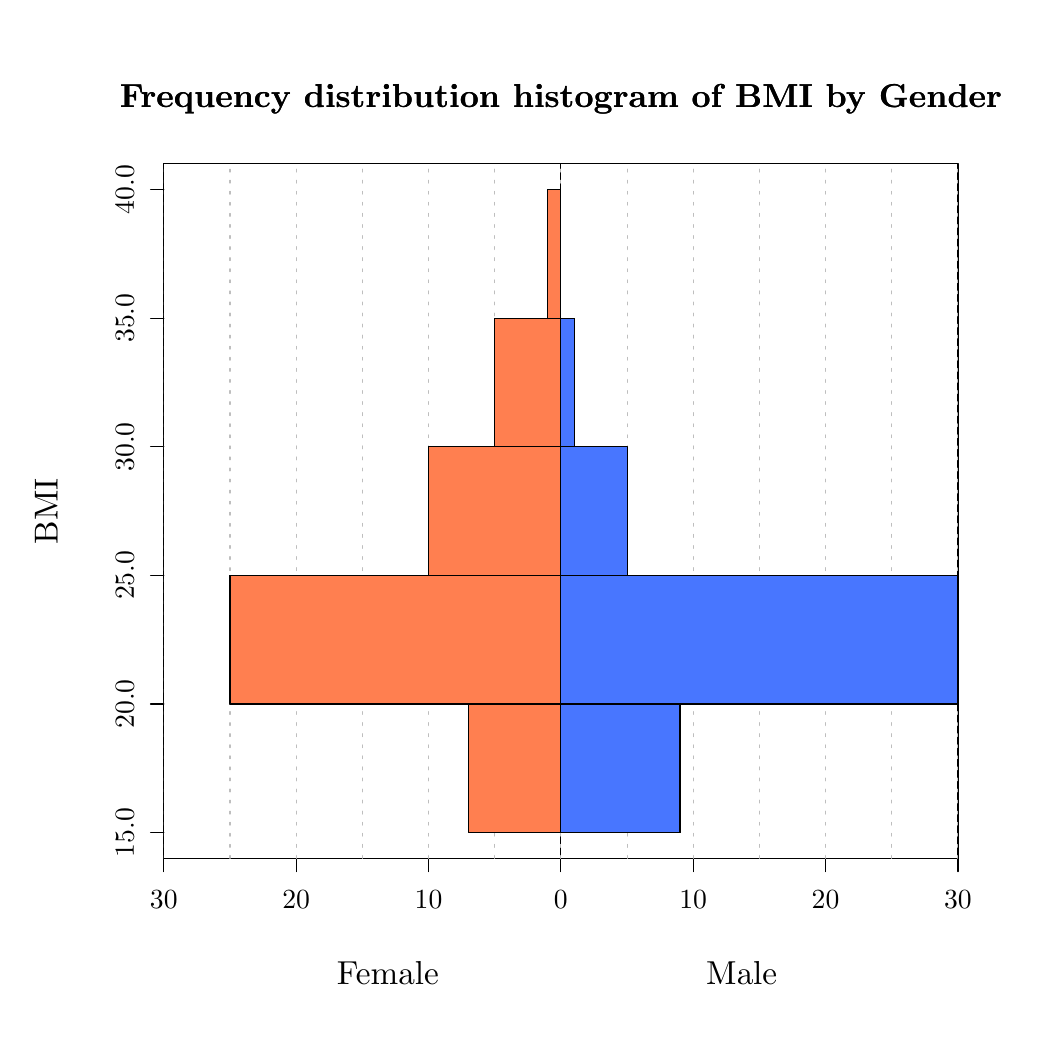
\begin{tikzpicture}[x=1pt,y=1pt]
\definecolor{fillColor}{RGB}{255,255,255}
\path[use as bounding box,fill=fillColor,fill opacity=0.00] (0,0) rectangle (361.35,361.35);
\begin{scope}
\path[clip] (  0.00,  0.00) rectangle (361.35,361.35);
\definecolor{drawColor}{RGB}{0,0,0}

\path[draw=drawColor,line width= 0.4pt,line join=round,line cap=round] (192.68, 70.49) rectangle (159.20,116.97);

\path[draw=drawColor,line width= 0.4pt,line join=round,line cap=round] (192.68,116.97) rectangle ( 73.11,163.44);

\path[draw=drawColor,line width= 0.4pt,line join=round,line cap=round] (192.68,163.44) rectangle (144.85,209.91);

\path[draw=drawColor,line width= 0.4pt,line join=round,line cap=round] (192.68,209.91) rectangle (168.76,256.38);

\path[draw=drawColor,line width= 0.4pt,line join=round,line cap=round] (192.68,256.38) rectangle (187.89,302.86);

\node[text=drawColor,anchor=base,inner sep=0pt, outer sep=0pt, scale=  1.20] at (192.68,332.61) {\bfseries Frequency distribution histogram of BMI by Gender};
\end{scope}
\begin{scope}
\path[clip] (  0.00,  0.00) rectangle (361.35,361.35);
\definecolor{drawColor}{RGB}{0,0,0}

\path[draw=drawColor,line width= 0.4pt,line join=round,line cap=round] (192.68, 70.49) rectangle (235.72,116.97);

\path[draw=drawColor,line width= 0.4pt,line join=round,line cap=round] (192.68,116.97) rectangle (336.15,163.44);

\path[draw=drawColor,line width= 0.4pt,line join=round,line cap=round] (192.68,163.44) rectangle (216.59,209.91);

\path[draw=drawColor,line width= 0.4pt,line join=round,line cap=round] (192.68,209.91) rectangle (197.46,256.38);

\path[draw=drawColor,line width= 0.4pt,line join=round,line cap=round] (192.68,256.38) rectangle (192.68,302.86);

\node[text=drawColor,anchor=base,inner sep=0pt, outer sep=0pt, scale=  1.20] at (192.68,332.61) {\bfseries Frequency distribution histogram of BMI by Gender};
\end{scope}
\begin{scope}
\path[clip] (  0.00,  0.00) rectangle (361.35,361.35);
\definecolor{drawColor}{RGB}{0,0,0}

\path[draw=drawColor,line width= 0.4pt,line join=round,line cap=round] ( 49.20, 61.20) -- (336.15, 61.20);

\path[draw=drawColor,line width= 0.4pt,line join=round,line cap=round] ( 49.20, 61.20) -- ( 49.20, 56.40);

\path[draw=drawColor,line width= 0.4pt,line join=round,line cap=round] ( 97.03, 61.20) -- ( 97.03, 56.40);

\path[draw=drawColor,line width= 0.4pt,line join=round,line cap=round] (144.85, 61.20) -- (144.85, 56.40);

\path[draw=drawColor,line width= 0.4pt,line join=round,line cap=round] (192.68, 61.20) -- (192.68, 56.40);

\path[draw=drawColor,line width= 0.4pt,line join=round,line cap=round] (240.50, 61.20) -- (240.50, 56.40);

\path[draw=drawColor,line width= 0.4pt,line join=round,line cap=round] (288.32, 61.20) -- (288.32, 56.40);

\path[draw=drawColor,line width= 0.4pt,line join=round,line cap=round] (336.15, 61.20) -- (336.15, 56.40);

\node[text=drawColor,anchor=base,inner sep=0pt, outer sep=0pt, scale=  1.00] at ( 49.20, 43.20) {30};

\node[text=drawColor,anchor=base,inner sep=0pt, outer sep=0pt, scale=  1.00] at ( 97.03, 43.20) {20};

\node[text=drawColor,anchor=base,inner sep=0pt, outer sep=0pt, scale=  1.00] at (144.85, 43.20) {10};

\node[text=drawColor,anchor=base,inner sep=0pt, outer sep=0pt, scale=  1.00] at (192.68, 43.20) { 0};

\node[text=drawColor,anchor=base,inner sep=0pt, outer sep=0pt, scale=  1.00] at (240.50, 43.20) {10};

\node[text=drawColor,anchor=base,inner sep=0pt, outer sep=0pt, scale=  1.00] at (288.32, 43.20) {20};

\node[text=drawColor,anchor=base,inner sep=0pt, outer sep=0pt, scale=  1.00] at (336.15, 43.20) {30};

\path[draw=drawColor,line width= 0.4pt,line join=round,line cap=round] ( 49.20, 70.49) -- ( 49.20,302.86);

\path[draw=drawColor,line width= 0.4pt,line join=round,line cap=round] ( 49.20, 70.49) -- ( 44.40, 70.49);

\path[draw=drawColor,line width= 0.4pt,line join=round,line cap=round] ( 49.20,116.97) -- ( 44.40,116.97);

\path[draw=drawColor,line width= 0.4pt,line join=round,line cap=round] ( 49.20,163.44) -- ( 44.40,163.44);

\path[draw=drawColor,line width= 0.4pt,line join=round,line cap=round] ( 49.20,209.91) -- ( 44.40,209.91);

\path[draw=drawColor,line width= 0.4pt,line join=round,line cap=round] ( 49.20,256.38) -- ( 44.40,256.38);

\path[draw=drawColor,line width= 0.4pt,line join=round,line cap=round] ( 49.20,302.86) -- ( 44.40,302.86);

\node[text=drawColor,rotate= 90.00,anchor=base,inner sep=0pt, outer sep=0pt, scale=  1.00] at ( 38.40, 70.49) {15.0};

\node[text=drawColor,rotate= 90.00,anchor=base,inner sep=0pt, outer sep=0pt, scale=  1.00] at ( 38.40,116.97) {20.0};

\node[text=drawColor,rotate= 90.00,anchor=base,inner sep=0pt, outer sep=0pt, scale=  1.00] at ( 38.40,163.44) {25.0};

\node[text=drawColor,rotate= 90.00,anchor=base,inner sep=0pt, outer sep=0pt, scale=  1.00] at ( 38.40,209.91) {30.0};

\node[text=drawColor,rotate= 90.00,anchor=base,inner sep=0pt, outer sep=0pt, scale=  1.00] at ( 38.40,256.38) {35.0};

\node[text=drawColor,rotate= 90.00,anchor=base,inner sep=0pt, outer sep=0pt, scale=  1.00] at ( 38.40,302.86) {40.0};
\end{scope}
\begin{scope}
\path[clip] (  0.00,  0.00) rectangle (361.35,361.35);
\definecolor{drawColor}{RGB}{0,0,0}

\node[text=drawColor,anchor=base,inner sep=0pt, outer sep=0pt, scale=  1.20] at (130.14, 15.60) {Female};

\node[text=drawColor,anchor=base east,inner sep=0pt, outer sep=0pt, scale=  1.20] at (270.83, 15.60) {Male};

\node[text=drawColor,rotate= 90.00,anchor=base,inner sep=0pt, outer sep=0pt, scale=  1.20] at ( 10.80,186.67) {BMI};
\end{scope}
\begin{scope}
\path[clip] ( 49.20, 61.20) rectangle (336.15,312.15);
\definecolor{drawColor}{RGB}{0,0,0}

\path[draw=drawColor,line width= 0.4pt,line join=round,line cap=round] (192.68, 61.20) -- (192.68,312.15);
\end{scope}
\begin{scope}
\path[clip] (  0.00,  0.00) rectangle (361.35,361.35);
\definecolor{drawColor}{RGB}{0,0,0}

\path[draw=drawColor,line width= 0.4pt,line join=round,line cap=round] ( 49.20, 61.20) --
	(336.15, 61.20) --
	(336.15,312.15) --
	( 49.20,312.15) --
	( 49.20, 61.20);
\end{scope}
\begin{scope}
\path[clip] ( 49.20, 61.20) rectangle (336.15,312.15);
\definecolor{drawColor}{RGB}{190,190,190}

\path[draw=drawColor,line width= 0.4pt,dash pattern=on 1pt off 3pt ,line join=round,line cap=round] (  1.38, 61.20) -- (  1.38,312.15);

\path[draw=drawColor,line width= 0.4pt,dash pattern=on 1pt off 3pt ,line join=round,line cap=round] ( 25.29, 61.20) -- ( 25.29,312.15);

\path[draw=drawColor,line width= 0.4pt,dash pattern=on 1pt off 3pt ,line join=round,line cap=round] ( 49.20, 61.20) -- ( 49.20,312.15);

\path[draw=drawColor,line width= 0.4pt,dash pattern=on 1pt off 3pt ,line join=round,line cap=round] ( 73.11, 61.20) -- ( 73.11,312.15);

\path[draw=drawColor,line width= 0.4pt,dash pattern=on 1pt off 3pt ,line join=round,line cap=round] ( 97.03, 61.20) -- ( 97.03,312.15);

\path[draw=drawColor,line width= 0.4pt,dash pattern=on 1pt off 3pt ,line join=round,line cap=round] (120.94, 61.20) -- (120.94,312.15);

\path[draw=drawColor,line width= 0.4pt,dash pattern=on 1pt off 3pt ,line join=round,line cap=round] (144.85, 61.20) -- (144.85,312.15);

\path[draw=drawColor,line width= 0.4pt,dash pattern=on 1pt off 3pt ,line join=round,line cap=round] (168.76, 61.20) -- (168.76,312.15);

\path[draw=drawColor,line width= 0.4pt,dash pattern=on 1pt off 3pt ,line join=round,line cap=round] (192.68, 61.20) -- (192.68,312.15);

\path[draw=drawColor,line width= 0.4pt,dash pattern=on 1pt off 3pt ,line join=round,line cap=round] (216.59, 61.20) -- (216.59,312.15);

\path[draw=drawColor,line width= 0.4pt,dash pattern=on 1pt off 3pt ,line join=round,line cap=round] (240.50, 61.20) -- (240.50,312.15);

\path[draw=drawColor,line width= 0.4pt,dash pattern=on 1pt off 3pt ,line join=round,line cap=round] (264.41, 61.20) -- (264.41,312.15);

\path[draw=drawColor,line width= 0.4pt,dash pattern=on 1pt off 3pt ,line join=round,line cap=round] (288.32, 61.20) -- (288.32,312.15);

\path[draw=drawColor,line width= 0.4pt,dash pattern=on 1pt off 3pt ,line join=round,line cap=round] (312.24, 61.20) -- (312.24,312.15);

\path[draw=drawColor,line width= 0.4pt,dash pattern=on 1pt off 3pt ,line join=round,line cap=round] (336.15, 61.20) -- (336.15,312.15);

\path[draw=drawColor,line width= 0.4pt,dash pattern=on 1pt off 3pt ,line join=round,line cap=round] (360.06, 61.20) -- (360.06,312.15);
\end{scope}
\begin{scope}
\path[clip] (  0.00,  0.00) rectangle (361.35,361.35);
\definecolor{drawColor}{RGB}{0,0,0}
\definecolor{fillColor}{RGB}{255,127,80}

\path[draw=drawColor,line width= 0.4pt,line join=round,line cap=round,fill=fillColor] (192.68, 70.49) rectangle (159.20,116.97);

\path[draw=drawColor,line width= 0.4pt,line join=round,line cap=round,fill=fillColor] (192.68,116.97) rectangle ( 73.11,163.44);

\path[draw=drawColor,line width= 0.4pt,line join=round,line cap=round,fill=fillColor] (192.68,163.44) rectangle (144.85,209.91);

\path[draw=drawColor,line width= 0.4pt,line join=round,line cap=round,fill=fillColor] (192.68,209.91) rectangle (168.76,256.38);

\path[draw=drawColor,line width= 0.4pt,line join=round,line cap=round,fill=fillColor] (192.68,256.38) rectangle (187.89,302.86);
\definecolor{fillColor}{RGB}{72,118,255}

\path[draw=drawColor,line width= 0.4pt,line join=round,line cap=round,fill=fillColor] (192.68, 70.49) rectangle (235.72,116.97);

\path[draw=drawColor,line width= 0.4pt,line join=round,line cap=round,fill=fillColor] (192.68,116.97) rectangle (336.15,163.44);

\path[draw=drawColor,line width= 0.4pt,line join=round,line cap=round,fill=fillColor] (192.68,163.44) rectangle (216.59,209.91);

\path[draw=drawColor,line width= 0.4pt,line join=round,line cap=round,fill=fillColor] (192.68,209.91) rectangle (197.46,256.38);

\path[draw=drawColor,line width= 0.4pt,line join=round,line cap=round,fill=fillColor] (192.68,256.38) rectangle (192.68,302.86);
\end{scope}
\end{tikzpicture}
}
\end{center}

\begin{enumerate}
\item Draw the pie chart for the gender.
\item In which group is more representative the mean of the BMI?
\item Calculate the mean for the whole sample.
\end{enumerate}
Use the following sums\\
Females: $\sum x_i=1160$ kg/m$^2$ \quad $\sum x_i^2 = 29050$ kg$^2$/m$^4$\\
Males: $\sum x_i=1002$ kg/m$^2$ \quad $\sum x_i^2 = 22781$ kg$^2$/m$^4$
}
%SOLUTION
{\begin{enumerate}[start=2]
\item $\bar{f} =24.17$ kg/m$^2$, $s_{f}^2=21.1806$ (kg/m$^2$)$^2$, $s_f=4.6$ kg/m$^2$ and $cv_f = 0.19$.\\
$\bar{m} =22.28$ kg/m$^2$, $s_{m}^2=9.9506$ (kg/m$^2$)$^2$, $s_m=3.15$ kg/m$^2$ and $cv_m = 0.14$.
Thus, the mean of males is more representative.
\item $\bar{x}=23.25$ kg/m$^2$.
\end{enumerate}
}
%RESOLUTION
{Lamemos $H$ a la variable que mide el índice de masa corporal para los hombres y $M$ para las mujeres.
\begin{enumerate}
\item A partir del histograma de frecuencias absolutas de las mujeres podemos obtener fácilmente las frecuencias absolutas de los intervalos mirando la altura de las barras, y a partir de las frecuencias absolutas podemos calcular el resto de frecuencias.
La tabla de frecuencias para las mujeres es:
\[
\begin{array}{|c|r|r|r|r|}
\hline
   M   & n_i &  f_i & N_i &  F_i \\
\hline
 15-20 &   7 & 0.15 &   7 & 0.15 \\
 20-25 &  25 & 0.52 &  32 & 0.67 \\
 25-30 &  10 & 0.21 &  42 & 0.88 \\
 30-35 &   5 & 0.10 &  47 & 0.98 \\
 35-40 &   1 & 0.02 &  48 & 1.00 \\
\hline
\mbox{Suma} & 48 & 1.00 & & \\
\hline
\end{array}
\]
Del mismo modo, a partir del histograma de frecuencias absolutas de los hombres obtenemos la tabla de frecuencias para hombres:
\[
\begin{array}{|c|r|r|r|r|}
\hline
   H   & n_i &  f_i & N_i &  F_i \\
\hline
 15-20 &   9 & 0.20 &   9 & 0.20 \\
 20-25 &  30 & 0.67 &  39 & 0.87 \\
 25-30 &   5 & 0.11 &  44 & 0.98 \\
 30-35 &   1 & 0.02 &  45 & 1.00 \\
\hline
\mbox{Suma} & 45 & 1.00 & & \\
\hline
\end{array}
\]

\item La variable Sexo sólo tiene dos categorías que son Hombre y Mujer, de modo que el diagrama de sectores asociado sólo tendrá dos sectores. La tabla de frecuencias de la variable sexo es:
\[
\begin{array}{|c|r|r|}
\hline
  \textrm{Sexo}  & n_i &   f_i \\
\hline
 \textrm{Mujer}  &  48 & 0.516 \\
\hline
 \textrm{Hombre} &  45 & 0.484 \\
\hline
  \textrm{Suma}  &  93 & 1.000 \\
\hline
\end{array}
\]
Así pues, para calcular el ángulo correspondiente a cada sector basta con multiplicar $360^{\circ}$ (el ángulo de la circunferencia completa) por la frecuencia relativa de cada categoría:
\[
\alpha_m=360^{\circ}0.516=186^{\circ}\qquad \alpha_h=360^{\circ}0.484=174^{\circ}.
\]
Y el diagrama de sectores asociados es:
\begin{center}
\includegraphics[scale=0.6]{img/sectores-des-29}
\end{center}

\item La media será más representativa en el grupo que tenga menos dispersión, y para comparar la dispersión de ambos grupos necesitamos el coeficiente de variación.
Calculamos para ello los estadísticos necesarios a partir de las tablas de frecuencias. Para las mujeres tenemos:
\[
\begin{array}{|c|r|r|r|r|}
\hline
   M   & m_i & n_i & m_in_i & m_i^2n_i \\
\hline
 15-20 & 17.5 &  7 & 122.5 & 2143.75 \\
 20-25 & 22.5 & 25 & 562.5 & 12656.25\\
 25-30 & 27.5 & 10 & 275.0 & 7562.50 \\
 30-35 & 32.5 &  5 & 162.5 & 5281.25 \\
 35-40 & 37.5 &  1 &  37.5 & 1406.25 \\
\hline
\mbox{Suma} & & 48 & 1160.0& 29050.00 \\
\hline
\end{array}
\]

\begin{align*}
\bar{m} & = \frac{\sum m_{i}}{n_m}=\frac{1160}{48}=24.17,  \\
s_{m}^2 &= \frac{\sum m_{i}^2}{n_m}-\bar{m}^2 = \frac{29050}{48}-24.17^2=21.1806,  \\
s_m &= \sqrt{21.1806} = 4.6,\\
cv_m &= \frac{s_m}{|\bar{m}|}=\frac{4.6}{24.17} = 0.19.
\end{align*}

Y para los hombres:
\[
\begin{array}{|c|r|r|r|r|}
\hline
   H   & h_i &  n_i & h_in_i &  h_i^2n_i \\
\hline
 15-20 &  17.5 &  9 & 157.5 &  2756.25 \\
 20-25 &  22.5 & 30 & 675.0 & 15187.50 \\
 25-30 &  27.5 &  5 & 137.5 &  3781.25 \\
 30-35 &  32.5 &  1 &  32.5 &  1056.25 \\
\hline
\mbox{Suma} & & 45 & 1002.5 & 22781.25 \\
\hline
\end{array}
\]

\begin{align*}
\bar{h} & = \frac{\sum h_{i}}{n_h}=\frac{1002.5}{45}=22.28,  \\
s_{h}^2 & = \frac{\sum h_{i}^2}{n_h}-\bar{h}^2 =
\frac{22781.25}{45}-22.28^2=9.9506,  \\
s_h &= \sqrt{9.9506} = 3.15,\\
cv_h &= \frac{s_h}{|\bar{h}|}=\frac{3.15}{22.28} = 0.14.
\end{align*}

Así pues, ambas muestras tienen un coeficiente de variación bajo y por tanto las medias son muy representativas, pero lo es un poco más la de los hombres ya que tienen una poca menos dispersión.

\item Para calcular la media de toda la muestra podemos hacer una media ponderada de las medias de las mujeres y l
os hombres donde los pesos son los tamaños muestrales de cada grupo.
\[
\bar{x}=\frac{p_m\bar{m}+p_h\bar{h}}{p_m+p_h}=\frac{45\cdot 22.28+48\cdot 24.17}{45+48}=23.25.
\]

\end{enumerate}
}


\newproblem*{des-30}{med}{*}
%STATEMENT
{Se ha medido el tiempo necesario, en días, para curar un tipo concreto de infección (tiempo transcurrido desde el comienzo del tratamiento hasta el alta) en dos grupos de pacientes a los que se han aplicado antibióticos diferentes.
En un grupo de 80 pacientes tratados con el antibiótico A, los resultados obtenidos fueron:
\[
\begin{array}{|c|c|}
\hline
\mbox{Tiempo (días)} & n_i \\
\hline
{[0,30)} & 50 \\
{[30,60)} & 20 \\
{[60,90)} & 10 \\
\hline
\end{array}
\]

Mientras que en un grupo de 100 pacientes tratados con el antibiótico B se obtuvo:
\[
\begin{array}{|c|c|}
\hline
\mbox{Tiempo (días)} & n_i \\
\hline
{[0,30)} & 40 \\
{[30,60)} & 50 \\
{[60,90)} & 10 \\
\hline
\end{array}
\]

\begin{enumerate}
\item Calcular la media y la desviación típica del número de días hasta el alta, para cada uno de los antibióticos.
\item ¿En qué antibiótico es más representativa la media?. Justificar la respuesta numéricamente.
\item ¿Cuánto vale el percentil 90 del tiempo de curación para los pacientes tratados con B?
\item ¿Qué tiempo de recuperación ha sido relativamente más alto, uno de 40 días de un paciente tratado con A, o uno de 45 días de otro tratado con B? Justificar la respuesta numéricamente.
\end{enumerate}
}


\newproblem{des-31}{med}{*}
%STATEMENT
{Para  estudiar la eficacia de un nuevo fármaco en el tratamiento de la hipertensión arterial, se tomaron los valores
de la tensión arterial diastólica (TAD) en 8 pacientes antes del tratamiento ($X$) y después de un mes de tratamiento
($Y$), obteniéndose los siguientes resultados:
\begin{center}
\begin{tabular}{|c|r|r|r|r|r|r|r|r|}
\hline
$X$ & 100 & 104 & 96 & 98 & 105 & 106 & 110 & 100 \\
\hline
$Y$ & 92 & 97 & 94 & 100 & 94 & 92 & 95 & 104 \\
\hline
\end{tabular}
\end{center}

\begin{enumerate}
\item ¿En qué variable es más representativa la media?
\item Hallar el coeficiente de asimetría de la variable $Y$ e interpretarlo.
\end{enumerate}
}
%SOLUTION
{\begin{enumerate}
\item $\bar x=102.375$, $s_x^2=18.9844$, $s_x=4.3571$ y $cv_x =0.0426$.\\
$\bar y=96$, $s_y^2=15.25$, $s_y=3.9051$ y $cv_y = 0.0407$.\\
Como ambos coeficientes de variación son casi iguales podemos concluir que ambas medias son igual de representativas.
\item $g_1=0.9068$ lo que indica que es asimétrica hacia la derecha.
\end{enumerate}
}
%RESOLUTION
{\begin{enumerate}
\item Para ver en qué muestra es más representativa la media tenemos que comparar las dispersiones de ambas muestras mediante el coeficiente de variación. Para ello, procedemos al cálculo de los estadísticos necesarios:
\begin{align*}
\bar{x} & = \frac{\sum x_{i}}{n}=\frac{100+\cdots+100}{8}=\frac{819}{8}=102.375,  \\
s_{x}^2 & = \frac{\sum x_{i}^2}{n}-\bar{x}^2 =
\frac{100^2+\cdots+100^2}{8}-102.375^2=\frac{83997}{8}-10480,6406=18.9844,  \\
s_{x} & = \sqrt{18.9844}=4.3571,  \\
cv_x &= \frac{s_x}{|\bar{x}|}= \frac{4.3571}{102.375}=0.0426,\\
\bar{y} & = \frac{\sum y_{j}}{n}=\frac{92+\cdots+104}{8}=
\frac{768}{8}=96,  \\
s_{y}^2 & = \frac{\sum y_{j}^2}{n}-\bar{y}^2 =
\frac{92^2+\cdots+104^2}{8}-96^2=\frac{73850}{8}-9216=15.25,  \\
s_{y} & = \sqrt{15.25}=3.9051,  \\
cv_y &= \frac{s_y}{|\bar{y}|}= \frac{3.9051}{96}=0.0407,\\
\end{align*}
Ambos coeficientes de variación son muy pequeños, lo cual indica que hay muy poca dispersión en las muestras y las medias son muy representativas, aunque un poco más la de $Y$ por tener un coeficiente de variación más pequeño.

\item El coeficiente de asimetría de $Y$ es
\[g_1=\frac{\sum(y_j-\bar{y})^3/n}{s_y^3}=
\frac{\left((92-96)^3+\cdots +(104-96)^3\right)/8}{3.9051^3}=\frac{432/8}{59,552}=0.9068,\]
lo que indica que la distribución es asimétrica a la derecha aunque no los suficiente como para rechazar la hipótesis de que los datos provienen de una población normal.
\end{enumerate}
}


\newproblem{des-32}{amb}{*}
%STATEMENT
{Una piscifactoría realiza un estudio para determinar si una especie de pez está en peligro extinción en los ríos de una región.
Para ello se midió el número de peces en 10 sitios diferentes obteniendo los siguientes resultados en unidades
por hectómetro cúbico:
\begin{center}
  36 -- 11 -- 7 -- 18 -- 35 -- 27 -- 21 -- 15 -- 25 -- 12
\end{center}
Se pide:
\begin{enumerate}
\item Calcular las medidas de tendencia central.
\item Calcular el coeficiente de apuntamiento e interpretarlo.
\end{enumerate}
}
%SOLUTION
{\begin{enumerate}
\item $\bar{x} = 20.7$ peces, $Me=19.5$ peces, no hay moda porque todos los valores tienen frecuencia 1.
\item $g_2= -1.13$ lo que indica que es una distribución bastante platicúrtica.
\end{enumerate}
}
%RESOLUTION
{Llamemos $X$ al número de peces por hectómetro cúbico.
\begin{enumerate}
\item Las medidas de tendencia central son la media aritmética, la mediana y la moda. Calculamos primero la media:
\[
\bar{x} = \frac{\sum x_{i}}{n}=\frac{36+\cdots+12}{10}=\frac{207}{10}=20.7 \mbox{ peces},
\]

Para calcular la mediana ordenamos los valores de la muestra:
\begin{center}
  7 -- 11 -- 12 -- 15 -- 18 -- 21 -- 25 -- 27 -- 35 -- 36
\end{center}
Como el tamaño de la muestra es par, habrá dos individuos que ocupen las posiciones centrales de la muestra, y estos serán los que ocupen las posiciones $n/2=10/2=5$ y $n/2+1=6$, es decir, los valores 18 y 21. Así pues la mediana es
\[
Me=\frac{18+21}{2}=19.5 \mbox{ peces}.
\]

Por último, no podemos decir que haya moda porque todos los valores tienen frecuencia 1.

\item La fórmula del coeficiente de apuntamiento es
\[
g_2=\frac{\sum (x_i-\bar{x})^4}{ns^4}-3,
\]
así que necesitamos calcular previamente la desviación típica:
\begin{align*}
s^2 & = \frac{\sum x_{i}^2}{n}-\bar{x}^2 =
\frac{36^2+\cdots+12^2}{10}-20.7^2=\frac{5179}{10}-428,49=89.41,\\
s &=\sqrt{89.41}=9.4557.
\end{align*}
Así pues, tenemos
\[
g_2=\frac{(36-20.7)^4+\cdots + (12-20.7)^4}{10\cdot 9.4557^4}-3=\frac{149449.657}{79941,9504}-3=-1.13,
\]
lo que indica que la distribución es bastante platicúrtica, es decir, con menos apuntamiento que una distribución normal.
\end{enumerate}
}


\newproblem{des-33}{amb}{*}
%STATEMENT
{Las temperaturas (en ºC) observadas en Barcelona y La Coruña en 12 días elegidos aleatoriamente el último año fueron:
\begin{center}
\begin{tabular}{|l|cccccccccccc|}
\hline
Barcelona & 13 & 14 & 16 & 18 & 21 & 25 & 28 & 28 & 25 & 21 & 17 & 13\\ \hline
La Coruña & 13 & 13 & 15 & 16 & 17 & 20 & 22 & 23 & 22 & 19 & 15 & 13\\ \hline
\end{tabular}
\end{center}
Se pide:

\begin{enumerate}
\item ¿En cuál de las dos ciudades hay mayor variación de temperaturas?
\item ¿Por debajo de qué valor estarán las temperaturas de la mitad de los días en ambas ciudades?
\end{enumerate}
}
%SOLUTION
{\begin{enumerate}
\item $cv_b = 0.2684$ y $cv_c =0.2071$ lo que indica que hay una ligera mayor variación de temperaturas en Barcelona.
\item $Me_b = 19,5.$ y $Me_c= 16.5$.
\end{enumerate}
}
%RESOLUTION
{Llamemos $B$ a la variable que mide las temperaturas en Barcelona, y $C$ a la que mide las temperaturas en La Coruña.
\begin{enumerate}
\item Para ver en qué ciudad hay mayor variación de temperatura tenemos que calcular los coeficientes de variación de ambas ciudades y compararlos.
\begin{align*}
\bar{b} &=\frac{\sum b_i}{n}= \frac{13+14+\cdots+13}{12}=\frac{239}{12}=19.9167,\\
s_b^2 &= \frac{\sum b_i^2}{n}-\bar{b}^2=\frac{13^2+14^2+\cdots+13^2}{12}-19.9167^2=\frac{5103}{12}-396.6749=28.5764,\\
s_b &=\sqrt{28.5764}=5.3457,\\
cv_b &= \frac{s_b}{|\bar{b}|}=\frac{5.3457}{19.9167}=0.2684,\\
\bar{c} &=\frac{\sum c_i}{n}= \frac{13+13+\cdots+13}{12}=\frac{208}{12}=17.3333,\\
s_c^2 &= \frac{\sum c_i^2}{n}-\bar{c}^2=\frac{13^2+13^2+\cdots+13^2}{12}-17.3333^2=\frac{3760}{12}-300.4433=12.8889,\\
s_c &=\sqrt{12.8889}=3.5901,\\
cv_c &= \frac{s_c}{|\bar{c}|}=\frac{3.5901}{17.3333}=0.2071.
\end{align*}
Por consiguiente, como el coeficiente de variación es mayor en Barcelona, es en esta ciudad donde hay mayor variación de temperaturas.

\item El valor que cumple que por debajo del mismo están la mitad de los valores de la muestra es la mediana.
Para calcular la mediana en ambas ciudades ordenamos los valores de la muestra de menor a mayor, y puesto que tenemos un tamaño muestral par $n=12$, buscamos los dos valores centrales, que ocuparan las posiciones $n/2=6$ y $n/2+1=7$.
En el caso de Barcelona tenemos que dichos valores son
\begin{center}
\begin{tabular}{|c|cccccccccccc|}
\hline
Posición & 1 & 2 & 3 & 4 & 5 & 6 & 7 & 8 & 9 & 10 & 11 & 12   \\ \hline
B & 13 & 13 & 14 & 16 & 17 & \fbox{18} & \fbox{21} & 21 & 25 & 25 & 28 & 28 \\ \hline
\end{tabular}
\end{center}
Como son valores diferentes, la mediana es $Me_b=\dfrac{18+21}{2}=19,5.$

En el caso de La Coruña tenemos
\begin{center}
\begin{tabular}{|c|cccccccccccc|}
\hline
Posición & 1 & 2 & 3 & 4 & 5 & 6 & 7 & 8 & 9 & 10 & 11 & 12   \\ \hline
C & 13 & 13 & 13 &  15 & 15 & \fbox{16} & \fbox{17} & 19 & 20 & 22 & 22 & 23 \\ \hline
\end{tabular}
\end{center}
Y al igual que antes, la mediana es $Me_c=\dfrac{16+17}{2}=16,5.$
\end{enumerate}
}


\newproblem{des-34}{gen}{*}
%STATEMENT
{Las pruebas de determinación del cociente intelectual realizadas en un colectivo de alumnos universitarios
reflejan los siguientes resultados:
\begin{center}
\begin{tabular}{|c|c|}
\hline
   C.I.    & Nº de alumnos \\
\hline
  [80,90)  &       3       \\
\hline
 [90,100)  &      12       \\
\hline
 [100,110) &      21       \\
\hline
 [110,120) &      24       \\
\hline
 [120,130) &      13       \\
\hline
 [130,140) &       2       \\
\hline
\end{tabular}
\end{center}
\begin{enumerate}
\item Calcular el coeficiente de variación del cociente intelectual. ¿Es representativa la media?
\item Si se considera ``muy inteligente'' a una persona cuyo cociente intelectual se encuentra en el 10\% de los más inteligentes, ¿cuál será el cociente que delimita la categoría ``muy inteligente'' en el colectivo de alumnos?
\end{enumerate}
}
%SOLUTION
{\begin{enumerate}
\item $cv=0.1$ lo que indica que hay poca dispersión y la media es muy representativa.
\item $P_{90}=125.77$.
\end{enumerate}
}
%RESOLUTION
{\begin{enumerate}
\item Para calcular el coeficiente de variación necesitamos la media y la desviación típica.
Para facilitar los cálculos, añadimos dos nuevas columnas a la tabla de distribución de frecuencias:
\[
\begin{array}{|c|c|r|r|r|}
\hline
   \textrm{C.I.}   & x_i & \multicolumn{1}{c|}{n_i} & \multicolumn{1}{c|}{x_in_i} & \multicolumn{1}{c|}{x_i^2n_i}\\
\hline\hline
  [80,90)  &  85  &   3       & 255 & 21675 \\
\hline
 [90,100)  &  95 &    12       & 1140 & 108300 \\
\hline
 [100,110) &  105 &    21       & 2205 & 231525\\
\hline
 [110,120) &  115 &    24       & 2760 & 317400\\
\hline
 [120,130) &  125 &    13       & 1625 & 203125\\
\hline
 [130,140) &  135 &     2       & 270 & 36450\\
\hline\hline
 \textrm{Sumas} &  & 75 & 8255 & 918475 \\
\hline
\end{array}
\]
A partir de aquí calculamos los estadísticos que necesitamos.
\begin{align*}
\bar{x} & = \frac{\sum x_in_i}{N}=\frac{8255}{75}=110.07,\\
s^2 & =\frac{\sum x_i^2n_i}{N}-\bar{x}^2= \frac{918475}{75}-110.07^2=131.6622,\\
s & =\sqrt{131.6622}=11.47.
\end{align*}
Finalmente calculamos el coeficiente de variación:
\[
cv=\frac{s}{|\bar{x}|}=\frac{11.47}{110.07}= 0.1.
\]
Puesto que el coeficiente de variación es pequeño, podemos concluir que hay poca dispersión en la muestra y por tanto, la media es representativa.

\item Buscamos el coeficiente intelectual por encima del cual está el 10\% más inteligente de la clase, o lo que es lo mismo, por debajo del cual está el 90\% menos inteligente de la clase. En definitiva se trata de calcular el percentil 90.
Para ello necesitamos la columna de frecuencias acumuladas en la tabla
\[
\begin{array}{|c|r|r|}
\hline
   \textrm{C.I.}    & \multicolumn{1}{c|}{n_i} & \multicolumn{1}{c|}{N_i} \\
\hline\hline
  [80,90)  &       3       & 3 \\
\hline
 [90,100)  &      12       & 15 \\
\hline
 [100,110) &      21       & 36 \\
\hline
 [110,120) &      24       & 60 \\
\hline
 [120,130) &      13       & 73 \\
\hline
 [130,140) &       2       & 75 \\
\hline
\end{array}
\]

La frecuencia acumulada correspondiente al percentil 90 es $N_{P_{90}}=90\cdot 75/100=67.5$. Mirando el la  columna de frecuencias acumuladas de la tabla de frecuencias comprobamos que dicha frecuencia se alcanza dentro del intervalo $[120,130)$.
Interpolando en este intervalo obtenemos el percentil que buscamos \[P_{90}=120+\frac{67.5-60}{13}10=125.77.\]
\end{enumerate}
}


\newproblem{des-35}{far}{*}
%STATEMENT
{En un laboratorio farmacéutico se van a fabricar dos tipos de cápsulas $A$ y $B$, cuyos contenidos en principio
activo debe ser 250 y 500 mg. respectivamente. Para ello se prueban dos máquinas dosificadoras, una para cada tipo de
cápsulas, siendo los contenidos en principio activo de las cápsulas fabricadas con ellas los siguientes:
\[
\begin{array}{c|c}
A & B  \\ \hline
238 & 488  \\
245 & 494  \\
236 & 476  \\
248 & 483  \\
241 & 492  \\
243 &
\end{array}
 \]
¿En cuál de las dos máquinas es más representativa la media?
Razonar la respuesta.
}
%SOLUTION
{$cv_{A} = 0.0167$ y $cv_{B}=0.0133$, luego es un poco más representativa la media en la máquina $B$.
}
%RESOLUTION
{Llamaremos $A$ a la variable que mide la cantidad de principio activo que pone la máquina $A$ en cada cápsula y $B$ a la variable que mide la cantidad de principio activo que pone la máquina $B$ en cada cápsula.
Para ver en cual de las dos muestras es más representativa la media, tenemos que calcular los coeficientes de variación en cada caso.

Calculamos primero los estadísticos necesarios para la máquina $A$:
\begin{align*}
\bar{A} & = \frac{\sum A_{i}}{n_{A}}=\frac{1451}{6}=241.833,\\
s_{A}^2 & =  \frac{\sum{A_{i}^2}{n_{A}}}-\bar{A}^2= \frac{350999}{6}-241.833^2=16.472,\\
s_{A} & = \sqrt{16.472}= 4.058,\\
cv_{A} & = \frac{s_{A}}{\bar{A}}=\frac{4.058}{241.833}=0.0167,
\end{align*}

En el caso de la máquina $B$ tenemos:
\begin{align*}
\bar{B} & = \frac{\sum B_{i}}{n_{B}}=\frac{2433}{5}=486.6,\\
s_{B}^2 & = \frac{\sum{B_{i}^2}{n_{B}}}-\bar{B}^2= \frac{1184109}{5}-486.6^2=42.24,\\
s_{B} & = \sqrt{42.24}= 6.499,\\
cv_{B} & = \frac{s_{B}}{\bar{B}}=\frac{6.499}{486.6}=0.0133.
\end{align*}

Como el coeficiente de variación de la muestra de $B$ es un poco menor que el de $A$, la dispersión será menor en la muestra de $B$ y $\bar{B}$ será un poco más representativa que $\bar{A}$.
}


\newproblem{des-36}{gen}{*}
%STATEMENT
{En un centro de reclutamiento se han medido las alturas de 150 jóvenes, obteniéndose la siguiente tabla de frecuencias:
\[
\begin{tabular}{|c|c|}
\hline
Altura: & Número de jóvenes: \\ \hline
1.50-1.60 & 12 \\ \hline
1.60-1.70 & 30 \\ \hline
1.70-1.80 & 52 \\ \hline
1.80-1.90 & 42 \\ \hline
1.90-2.00 & 11 \\ \hline
2.00-2.10 & 3 \\ \hline
\end{tabular}
\]

\begin{enumerate}
\item Calcular el coeficiente de variación. ¿Es representativa la media?
\item  Si se considera alto a un joven cuya altura corresponde como mínimo a la del percentil 85, ¿cuál es la
mínima altura que tendrá un alto?
\end{enumerate}
}
%SOLUTION
{\begin{enumerate}
\item $cv=0.065$ lo que indica muy poca dispersión y una media muy representativa.
\item $ P_{85}=1.88$ mt.
\end{enumerate}
}
%RESOLUTION
{\begin{enumerate}
\item  El coeficiente de variación se define como
\[
cv=\dfrac{s}{|\bar{x}|},
\]
de modo que necesitamos calcular la media y la desviación típica, pero antes de nada, completamos la tabla de frecuencias.
\[
\begin{array}{|c|c|c|c|c|}
\hline
x_{i} & n_{i} & N_{i} & x_{i}n_{i} & x_{i}^2n_{i}\\ \hline
1.50-1.60 & 12 & 12 & 18.6 & 28.83 \\
1.60-1.70 & 30 & 42 & 49.5 & 81.68 \\
1.70-1.80 & 52 & 94 & 91 & 159.25\\
1.80-1.90 & 42 & 136 & 77.7 & 143.75\\
1.90-2.00 & 11 & 147 & 21.45 & 41.83\\
2.00-2.10 & 3 & 150 & 6.15 & 12.61\\ \hline
\mbox{Sumas} & 150 & & 264.4 & 467.94 \\
\hline
\end{array}
\]
Ahora calculamos la media y la desviación típica:
\begin{eqnarray*}
\bar{x} & = & \frac{\sum
x_{i}n_{i}}{N}=\frac{264.4}{150}=1.7627.\\
s^2 & = & \frac{\sum x_{i}^2 n_{i}}{N}-\bar{x}^2 =
\frac{467.94}{150}-1.7627^2=0.013.\\
s & = & \sqrt{0.02}=0.114.
\end{eqnarray*}
Por consiguiente, el coeficiente de variación es
\[ cv=\frac{0.114}{1.7627}=0.065, \]
lo que indica que hay muy poca dispersión y la media es muy representativa.

\item Tenemos que calcular el percentil 85 para ver a partir de qué estatura un joven es considerado alto.
La frecuencia absoluta acumulada correspondiente al percentil 85 es $85\cdot N/100=85\cdot 150/100 = 127.5$.
Mirando la tabla de frecuencias en la columna de las frecuencias absolutas acumuladas podemos comprobar que la frecuencia 127.5 se alcanza en algún punto del intervalo 1.80-1.90.
Para obtener el percentil 85 interpolamos en dicho intervalo:
\[ P_{85}=1.80+\frac{127.5-94}{42}(1.90-1.80)=1.88. \]
\end{enumerate}
}


\newproblem{des-37}{med}{*}
%STATEMENT
{Se ha realizado un estudio sobre la tensión arterial en dos ciudades A y B. Se tomó una muestra de 20 individuos, que arrojó los siguientes valores:
\begin{center}
\begin{tabular}{l}
\begin{tabular}{|l|c|c|c|c|c|c|c|c|c|c|}
\hline
 Tensión & 135 & 128 & 137 & 110 & 154 & 142 & 121 & 127 & 114 & 103 \\
\hline
 Ciudad  &  A  &  B  &  A  &  B  &  A  &  A  &  A  &  B  &  B  &  B  \\
\hline
\end{tabular}
\\[.5cm]
\begin{tabular}{|l|c|c|c|c|c|c|c|c|c|c|}
\hline
 Tensión & 98 & 96 & 114 & 123 & 132 & 141 & 132 & 121 & 98 & 136 \\
\hline
 Ciudad  & A  & B  &  A  &  B  &  A  &  B  &  A  &  B  & B  &  A  \\
\hline
\end{tabular}
\end{tabular}
\end{center}
Se pide:
\begin{enumerate}
\item Construir la tabla de frecuencias para la tensión, agrupando en clases de amplitud 10, entre 95 y 155.
\item Dibujar el polígono de frecuencias acumuladas correspondiente a la tabla anterior.
\item Calcular el coeficiente de asimetría e interpretarlo.
\item Calcular el tercer decil e interpretarlo.
\item Considerando los datos sin agrupar, ¿en qué ciudad son más homogéneas las tensiones?
\end{enumerate}
}
%SOLUTION
{\begin{enumerate}[start=3]
\item $\bar x = 123$ mmHg, $s^2= 251$ mmHg$^2$, $s=15.843$ mmHg y $g_1=-0.12$, por lo que la distribución es un poco asimétrica hacia la izquierda.
\item $D_3= 111,67$ mmHg.
\item $\bar x_A=130.1$ mmHg, $s^2_A=219.89$ mmHg$^2$, $s_A=14.8287$ mmHg y $cv_A =0.1139$.\\
$\bar x_B=116.1$ mmHg, $s^2_B=189.69$ mmHg$^2$, $s_B=13.7728$ mmHg y y $cv_B = 0.1186$.
Así pues, como el $cv_A<cv_B$ las tensiones son un poco más homogéneas en la ciudad $A$, aunque en ambos casos las muestras son muy homogéneas.
\end{enumerate}
}
%RESOLUTION
{Llamemos $X$ a la variable que mide la tensión arterial.
\begin{enumerate}
\item Agrupando en clases de amplitud 10, obtenemos 6 clases entre 95 y 155. La tabla de frecuencias correspondiente es
\[
\begin{array}{|c|r|r|r|r|r|}
\hline
   X  & \multicolumn{1}{c|}{x_i} & \multicolumn{1}{c|}{n_i} & \multicolumn{1}{c|}{f_i} & \multicolumn{1}{c|}{N_i} & \multicolumn{1}{c|}{F_i}\\
\hline\hline
  [95,105)  &  100  &   4       & 0.2 & 4 & 0.2\\
\hline
 [105,115)  &  110 &    3       & 0.15 & 7 & 0.35 \\
\hline
 [115,125) &  120 &    3       & 0.15 &  10 & 0.5\\
\hline
 [125,135) &  130 &    4       & 0.2 & 14 & 0.7\\
\hline
 [135,145) &  140 &    5       & 0.25 & 19 & 0.95\\
\hline
 [145,155) &  150 &     1       & 0.05 & 10 & 1\\
\hline
\end{array}
\]

\item El polígono de frecuencias absolutas acumuladas correspondiente a esta tabla es el siguiente
\begin{center}
\includegraphics[scale=0.6]{img/poligono-tension-des-37}
\end{center}

\item El coeficiente de asimetría se calcula mediante la fórmula
\[g_1=\frac{\sum (x-\bar{x})^3n_i/n}{s^3}.\]
A partir de la tabla anterior, calculamos los estadísticos necesarios:
\[
\begin{array}{|c|r|r|r|r|}
\hline
   X  & \multicolumn{1}{c|}{x_i} & \multicolumn{1}{c|}{n_i} & \multicolumn{1}{c|}{x_in_i} & \multicolumn{1}{c|}{x_i^2n_i}\\
\hline\hline
  [95,105)  &  100  &   4       & 400 & 40000\\
\hline
 [105,115)  &  110 &    3       & 330 & 36300 \\
\hline
 [115,125) &  120 &    3       & 360 &  43200\\
\hline
 [125,135) &  130 &    4       & 520 & 67600 \\
\hline
 [135,145) &  140 &    5       & 700 & 98000 \\
\hline
 [145,155) &  150 &     1       & 150 & 22500\\
\hline
\hline
\textrm{Sumas} & & 20 & 2460 & 307600\\
\hline
\end{array}
\]

\begin{align*}
\bar{x} & = \frac{\sum x_in_i}{n}=\frac{2460}{20}=123,\\
s^2 & =\frac{\sum x_i^2n_i}{N}-\bar{x}^2= \frac{307600}{20}-123^2=251,\\
s & =\sqrt{251}=15.84.
\end{align*}

Por último calculamos el coeficiente de asimetría
\[
\begin{array}{|c|r|r|r|r|}
\hline
   X  & \multicolumn{1}{c|}{x_i} & \multicolumn{1}{c|}{n_i} & \multicolumn{1}{c|}{x_i-\bar{x}} & \multicolumn{1}{c|}{(x_i-\bar{x})^3n_i}\\
\hline\hline
  [95,105)  &  100  &   4       & -23 & -48668\\
\hline
 [105,115)  &  110 &    3       & -13 & -6591 \\
\hline
 [115,125) &  120 &    3       & -3 &  -81\\
\hline
 [125,135) &  130 &    4       & 7 & 1372 \\
\hline
 [135,145) &  140 &    5       & 17 & 24565 \\
\hline
 [145,155) &  150 &     1       & 27 & 19683\\
\hline
\hline
\textrm{Sumas} & & 20 &  & -9720\\
\hline
\end{array}
\]

\[
g_1=\frac{\sum (x-\bar{x})^3n_i/n}{s^3}=\frac{-9720/20}{15.84^3}=-0.12.
\]
Esto indica que la distribución es ligeramente asimétrica a la izquierda.

\item El tercer decil $D_3$ tiene frecuencia absoluta acumulada $N_{D_3}=3n/10=3\cdot 20/10=6$, y mirando en la columna de frecuencias absolutas acumuladas comprobamos que corresponderá a un individuo de la clase $[105,115)$. Interpolando en dicho intervalo tenemos que que el tercer decil es
\[ D_3=105+\frac{6-4}{3}10=111,67,
\]
lo cual indica que  el 30\% de la población tiene un tensión inferior a 111.67.

\item Llamemos $a$ y $b$ a las variables que miden las tensiones de las ciudades A y B respectivamente. Las tensiones serán más homogéneas en la ciudad que haya menos dispersión. Para comparar las dispersiones de ambas poblaciones utilizamos el coeficiente de variación que no depende de las unidades. Calculamos los estadísticos necesarios trabajando directamente desde la muestra sin agrupar:
\begin{align*}
\bar{a} & = \frac{\sum a_{i}}{n}=\frac{135+\cdots+136}{10}=\frac{1301}{10}=130.1,  \\
s_{a}^2 & = \frac{\sum a_{i}^2}{n}-\bar{a}^2 =
\frac{135^2+\cdots+136^2}{10}-130.1^2=\frac{171459}{10}-16926.01=219.89,  \\
s_{a} & = \sqrt{219.89}=14.83,  \\
cv_a &=\frac{s_a}{|\bar{a}|}=\frac{14.83}{130.1}=0.1139,\\
\bar{b} & = \frac{\sum b_{j}}{n}=\frac{128+\cdots+98}{10}=
\frac{1161}{10}=116.1,  \\
s_{b}^2 & = \frac{\sum b_{j}^2}{n}-\bar{b}^2 =
\frac{128^2+\cdots+98^2}{10}-116.1^2=\frac{136689}{10}-13479.21=189.69,  \\
s_{b} & = \sqrt{189.69}=13.77,  \\
cv_b &=\frac{s_b}{|\bar{b}|}=\frac{13.77}{116.1}=0.1186.
\end{align*}
Así pues, comparando los coeficientes de variación en ambas ciudades comprobamos que son prácticamente iguales aunque es un poco menor la dispersión en la ciudad A por lo que las tensiones serán un poco más homogéneas.
\end{enumerate}
}


\newproblem{des-38}{gen}{*}
%STATEMENT
{En un grupo de alumnos se ha medido el número de días que faltaron a clase una muestra de alumnos de primer año y otra de alumnos repetidores, obteniendo:
\[
\begin{array}{lcccccccc}
\mbox{Primer año:}  & 8 & 2 & 3  & 2  & 1  & 4 & 0 & 3 \\
\mbox{Repetidores:} & 4 & 6 & 20 & 12 & 16 & 8 & 5 &   \\
\end{array}
\]
Se pide:
\begin{enumerate}
\item Calcular la mediana en ambos casos.
\item ¿En cuál de las dos muestras hay menos dispersión?
\item ¿Comparar el apuntamiento de ambas muestras?
\end{enumerate}
}
%SOLUTION
{\begin{enumerate}
\item $Me_{x}=2.5$ y $Me_{y}=8$.
\item $cv_x =0.7862$ y $cv_y =0.5538$, hay menos dispersión en los alumnos repetidores.
\item $g_{2_x} =0.703$ y $g_{2_y} =-1.125$ lo que indica que la distribución de los alumnos de primer año es leptocúrtica y la de los repetidores platicúrtica.
\end{enumerate}
}
%RESOLUTION
{Llamemos $X$ a la variable que mide el número de días que faltaron los alumnos de primer año, e $Y$ al de los alumnos repetidores
\begin{enumerate}
\item Para calcular la mediana primero ordenamos los datos de ambas muestras:
\[
\begin{array}{lcccccccc}
\mbox{Primer año:}  & 0 & 1 & 2  & 2  & 3  & 3 & 4 & 8 \\
\mbox{Repetidores:} & 4 & 5 & 6 & 8 & 12 & 16 & 20 &   \\
\end{array}
\]
En el primer caso, como el tamaño de la muestra es par, habrá dos valores que estarán en el centro de la distribución, que serán los que ocupen la posiciones $n/2=8/2=4$ y $n/2+1=5$, es decir, los valores 2 y 3, de modo que la mediana es su media:
\[
Me_{x}=\frac{2+3}{2}=2.5.
\]
En el segundo caso, como el tamaño muestral es impar, sólo habrá un valor central que será el que ocupe la posición $(n+1)/2=8/2=4$, es decir, el valor 8, y por tanto $Me_{y}=8$.

\item Para compara la dispersión de ambas muestras tenemos que calcular el coeficiente de variación, y para ello, previamente hay que calcular la media y la desviación típica de cada muestra:
\begin{align*}
\bar{x} & = \frac{\sum x_{i}}{n}=\frac{8+\cdots+3}{8}=\frac{23}{8}=2.875,  \\
s_{x}^2 & = \frac{\sum x_{i}^2}{n}-\bar{x}^2 =
\frac{8^2+\cdots+3^2}{8}-2.875^2=\frac{107}{8}-8,2656=5.1094,  \\
s_{x} & = \sqrt{5.1094}=2.2604,  \\
cv_x &=\frac{s_x}{|\bar{x}|}=\frac{2.2604}{2.875}=0.7862,\\
\bar{y} & = \frac{\sum y_{j}}{n}=\frac{4+\cdots+5}{7}=
\frac{71}{7}=10.143,  \\
s_{y}^2 & = \frac{\sum y_{j}^2}{n}-\bar{y}^2 =
\frac{4^2+\cdots+5^2}{7}-10.143^2=\frac{941}{7}-102.8804=31.5510,  \\
s_{y} & = \sqrt{31.5510}=5.617,  \\
cv_y &=\frac{s_y}{|\bar{y}|}=\frac{5.617}{10.143}=0.5538.
\end{align*}
Así pues, como el coeficiente de variación es menor en $Y$, hay menos dispersión el grupo de los repetidores.

\item El coeficiente de apuntamiento en ambas muestras es
\begin{align*}
g_{2_x} &=\frac{\sum (x_i-\bar{x})^4}{ns_x^4}-3= \frac{(8-2.875)^4+\cdots + (3-2.875)^4}{8\cdot 2.2604^4}-3=\frac{773.3379}{208.8484}-3=0.703,\\
g_{2_y} &=\frac{\sum (y_j-\bar{y})^4}{ns_y^4}-3= \frac{(4-10.143)^4+\cdots + (5-10.143)^4}{7\cdot 5.617^4}-3=\frac{13068.6239}{6968.1218}-3=-1.125.
\end{align*}
Por tanto, la primera muestra tiene un apuntamiento mayor de lo normal (leptocúrtica) mientras que la segunda muestra tiene un apuntamiento bastante menor de lo normal (platicúrtica).
\end{enumerate}
}


\newproblem*{des-39}{nut}{*}
%STATEMENT
{Al realizar un estudio sobre el peso de las mujeres mayores de 30 años en una determinada población, se obtuvieron los siguientes datos:
\begin{center}
72 -- 66 -- 51 -- 87 -- 65 -- 57 -- 73 -- 84 -- 67 -- 78 \\
58 -- 62 -- 75 -- 56 -- 68 -- 74 -- 57 -- 65 -- 73 -- 67
\end{center}
Realizar un estudio descriptivo agrupando los datos en 4 clases de amplitud 10 comenzando en el 50, que incluya:
\begin{enumerate}
\item Histograma de frecuencias absolutas y frecuencias absolutas acumuladas y los correspondientes polígonos.
\item Rango intercuartílico e interpretación.
\item Estudiar la representatividad de la media.
\end{enumerate}
}


\newproblem*{des-40}{nut}{*}
%STATEMENT
{Se realiza un estudio sobre el nivel de colesterol en sangre de los trabajadores de una empresa que utilizan habitualmente el comedor de la misma. Los resultados fueron los siguientes:
\begin{center}
214 - 205 - 197 - 204 - 186 - 192 - 216 - 176 - 192 - 196\\
207 - 182 - 218 - 203 - 194 - 176 - 203 - 214 - 188 - 198
\end{center}
Se pide:

\begin{enumerate}
\item Obtener la distribución de frecuencias agrupadas en clases de amplitud 10, comenzando en 170.
\item Dibujar el histograma y el polígono de frecuencias.
\item Calcular el coeficiente de variación de Pearson e interpretar los resultados.
\item Calcular el rango intercuartílico.
\end{enumerate}
}


\newproblem{des-41}{psi}{}
%STATEMENT
{En un grupo de alumnos universitarios se realiza un estudio sobre la velocidad de lectura.
Para ellos se les dio a leer un texto de un periódico y se contó el número de palabras que leyeron en un minuto, obteniendo los siguientes resultados:
\begin{center}
286 -- 242 -- 185 -- 244 -- 296 -- 211 -- 233 -- 179 -- 190 -- 274 \\
255 -- 222 -- 260 -- 216 -- 204 -- 247 -- 232 -- 257 -- 196 -- 261
\end{center}
Se pide:
\begin{enumerate}
\item Construir la tabla de frecuencias agrupando en intervalos de amplitud 25 comenzando en 175.
\item Calcular las medidas de tendencia central. ¿Es representativa la media?
\item Calcular el coeficiente de apuntamiento e interpretarlo.
\end{enumerate}
}
%SOLUTION
{\begin{enumerate}[start=2]
\item $\bar{x}=233.75$, $Med=235$, $Mod= [225,250)$ y $[250-275]$. $s^2=1017.19$, $s=31.89$ y $cv=0.14$ lo que indica que hay poca dispersión y la media es muy representativa.
\item $g_2=-1.1$ de manera que la distribución es bastante platicúrtica.
\end{enumerate}
}
%RESOLUTION
{}


\newproblem*{des-42}{amb}{*}
%STATEMENT
{Una piscifactoría realiza un estudio para determinar si una especie de pez está en peligro extinción en los ríos de una región.
Para ello se midió el número de peces en 12 sitios diferentes obteniendo los siguientes resultados en unidades por hectómetro cúbico:
\begin{center}
  16 -- 11 -- 14 -- 18 -- 21 -- 27 -- 21 -- 15 -- 22 -- 12 -- 2 -- 19
\end{center}
Se pide:
\begin{enumerate}
\item Dibujar el diagrama de cajas y eliminar de la muestra los datos atípicos si existen.
\item Calcular las medidas de tendencia central. ¿Cuál de ellas es más representativa?
\item Calcular el coeficiente de apuntamiento e interpretarlo.
\end{enumerate}
}


\newproblem*{des-43}{gen}{*}
%STATEMENT
{Dado el siguiente polígono correspondiente a una muestra de 60 individuos
\begin{center}
\includegraphics[scale=0.5]{img/poligono-acumuladas-des-43}
\end{center}
Calcular:
\begin{enumerate}
\item Tabla de frecuencias
\item Coeficiente de variación. ¿Se puede decir que hay mucha dispersión?
\item Decil 7.
\item Coeficiente de asimetría e interpretarlo.
\end{enumerate}
}


\newproblem*{des-44}{amb}{*}
%STATEMENT
{La siguiente tabla muestra los datos de emisiones de CO$_2$ y CH$_4$ (en kg/hab) y el producto interior bruto per cápita (en miles US\$) de varios países en el último año:
\[
\begin{array}{|l|r|r|r|}
\hline
\mbox{País} & \mbox{CO}_2 & \mbox{CH}_4 & \mbox{PIB}\\
\hline\hline
\mbox{Austria}     & 7.60 & 0.97 & 38.40\\ \hline
\mbox{España}      & 6.73 & 0.81	& 30.12\\ \hline
\mbox{Francia}     & 5.71 & 0.94	& 33.19\\ \hline
\mbox{EEUU}        &19.40 & 1.72	&	45.84\\ \hline
\mbox{Alemania}    & 9.80 & 0.83	& 34.18\\ \hline
\mbox{Canadá}      &15.60 & 3.08	& 38.43\\ \hline
\mbox{Italia}      & 7.29 & 0.58	& 30.44\\ \hline
\mbox{Japón}       &	9.44 & 0.16	& 33.58\\ \hline
\mbox{Australia}   &17.48 & 6.36	& 36.26\\ \hline
\mbox{Reino Unido} & 8.99 & 0.76	& 35.13\\ \hline
\end{array}
\qquad
\begin{array}{|l|r|r|r|}
\hline
\mbox{País} & \mbox{CO}_2 & \mbox{CH}_4 & \mbox{PIB}\\
\hline\hline
\mbox{Bolivia}     & 1.05 & 3.44	& 40.13\\ \hline
\mbox{Niger}       &	0.1	 & 0.12	&	 0.67\\ \hline
\mbox{Senegal}     &	0.35 & 0.76 &  1.69\\ \hline
\mbox{Pakistán}    & 0.65 & 0.59	&  2.59\\ \hline
\mbox{Filipinas}   &	0.83 & 0.46	&  3.38\\ \hline
\mbox{Perú}        & 0.94 & 0.75	&  7.80\\ \hline
\mbox{Túnez}      & 2.17 & 0.48	&  7.47\\ \hline
\mbox{Nepal}       & 0.13 & 0.90	&  1.21\\ \hline
\mbox{Nicaragua}   & 0.7	 & 0.32	&  2.62\\ \hline
\mbox{Mauritania}  & 0.97 & 0.85	&  2.01\\ \hline
\end{array}
\]
Se pide:
Agrupar los datos de CH$_4$ en 5 clases desde el 0 hasta el 2 y calcular:
\begin{enumerate}
\item Media, varianza y coeficiente de variación. ¿Existe mucha dispersión? Justificar la respuesta.
\item Calcular el Rango Intercuartílico e interpretarlo.
\item Tipificar los datos y calcular el coeficiente de asimetría e interpretarlo.
\end{enumerate}
}


\newproblem{des-45}{amb}{}
%STATEMENT
{Se realizó una encuesta a 40 personas de más de 70 años sobre el número de medicamentos distintos que tomaban habitualmente.
El resultado de dicha encuesta fue el siguiente:
\begin{center}
3 -- 1 -- 2 -- 2 -- 0 -- 1 -- 4 -- 2 -- 3 -- 5 -- 1 -- 3 -- 2 -- 3 -- 1 -- 4 -- 2 -- 4 -- 3 -- 2 \\
3 -- 5 -- 0 -- 1 -- 2 -- 0 -- 2 -- 3 -- 0 -- 1 -- 1 -- 5 -- 3 -- 4 -- 2 -- 3 -- 0 -- 1 -- 2 -- 3
\end{center}
Se pide:
\begin{enumerate}
\item Obtener la distribución de frecuencias de la muestra.
\item Dibujar el diagrama de barras y el polígono de frecuencias asociados.
\item Dibujar el diagrama de frecuencias acumuladas.
\item Calcular la media aritmética, la mediana y la moda.
\item Calcular la varianza y la desviación típica.
\item Calcular el coeficiente de variación de Pearson.
\end{enumerate}
}
%SOLUTION
{\begin{enumerate}[start=4]
\item $ \bar{x} = 2.225$, $Med =2$ y $Mod= 2$.
\item $s^2 = 1.974$, $s= 1.405$.
\item $cv = 0.632$.
\end{enumerate}
}
%RESOLUTION
{}


\newproblem*{des-46}{gen}{*}
%STATEMENT
{Se considera la variable estadística agrupada en clases cuya distribución de frecuencias viene dada por la siguiente tabla:
\[
\begin{array}{|c|c|c|c|c|}
\hline
X & n_i & f_i & N_i & F_i\\
\hline
[0,20) & & 0.25 & &  \\
\hline
[20,40) & & 0,3 & & \\
\hline
[40,60) &  &  & &  0,9\\
\hline
[60,80) & 6 & & & \\
\hline
\end{array}
\]

\begin{enumerate}
\item Completar razonadamente la tabla.
\item Hallar el rango intercuartílico e interpretarlo.
\item Hallar el coeficiente de apuntamiento e interpretarlo.
\end{enumerate}
}


\newproblem{des-47}{gen}{*}
%STATEMENT
{Se han medido las estaturas, $X$, en metros de 15 individuos, obteniéndose los siguientes sumatorios:
\[
\sum\limits_{i = 1}^{15} {x_i  = 26.40\;} {\rm m}{\rm ,}\;\sum\limits_{i = 1}^{15} {x^2 _i  = 52.45\;{\rm m}^{\rm 2} } ,\;\sum\limits_{i = 1}^{15} {\left( {x_i  - \bar x} \right)^3 }  =  - 8.42\;{\rm m}^3
\]

Se pide:
\begin{enumerate}
\item Calcular media, desviación típica, coeficiente de variación y coeficiente de asimetría de la variable. Interpretar los dos últimos.
\item Si trabajamos con una nueva variable $Y=1.1X-0.2$, ¿cuánto valdrán los estadísticos anteriores? Justificar adecuadamente la respuesta.
\end{enumerate}
}
%SOLUCION
{\begin{enumerate}
\item $\bar x=1.76\; \mbox{m}$, $s^2=0.399\;\mbox{m}^2$, $s=0.631\;\mbox{m}$, $CV=0.359$ (dispersión moderada), $g_1=- 2.234$ (distribución muy asimétrica a la izquierda)
\item $\bar y=1.736$, $s_y=0.694$, $CV_y=0.40$, $g_{1y}=-2.234$.
\end{enumerate}
}
%RESOLUTION
{\begin{enumerate}
\item Teniendo en cuenta los sumatorios que nos dan como datos, y el número total de datos en la muestra ($n=15$), obtenemos:
\begin{align*}
\bar x &= \frac{{\sum {x_i } }}{n} = \frac{{26.40}}{15} = 1.76\; \mbox{m},\\
s ^2  &= \frac{{\sum {x_i ^2 } }}{n} - \bar x^2  = \frac{{52.45}}{15} - 1.76^2  =0.399\;\mbox{m}^2,\\
s &=  + \sqrt {s^2 }  =  + \sqrt {0.399}  = 0.631\;\mbox{m},\\
CV &= \frac{s}{{\left| {\bar x} \right|}} = \frac{{0.631}}{{1.76}} = 0.359 = 35.9,\\
g_1 &= \frac{{\frac{{\sum {\left( {x_i  - \bar x} \right)^3 } }}{n}}}{{s^3 }} = \frac{{\frac{{ - 8.42}}{{15}}}}{{0.631^3 }} =  - 2.234.
\end{align*}

En cuanto a la interpretación del coeficiente de variación, su valor es igual a $0.359$, lo cual indica que la dispersión relativa en torno a la media es considerable (supera el 30\%), por lo que la media no es demasiado representativa de la distribución. Para el coeficiente de asimetría hemos obtenido un valor de $-2.234$, negativo lo cual indica que la distribución presenta cola a la izquierda.

\item Si tenemos una nueva variable obtenida mediante la transformación lineal: $Y=1.1 X -0.2$, le podemos aplicar el teorema que nos dice cuáles serán la nueva media y desviación típica de una variable $Y$ obtenida mediante una transformación lineal aplicada a otra $X$. Este teorema dice que si $Y=aX+b$, entonces $\bar y=a \bar x +b$, y $s_y = \left| a \right| s_x$. Por lo tanto:
\[
\bar y = 1.1 \cdot \bar x - 0.2 = 1.736,\qquad s_y  = 1.1 \cdot s_x  = 0.694.
\]

Con los resultados anteriores, el coeficiente de variación de la nueva variable resulta muy sencillo de calcular:
\[
CV_y = \frac{s_y}{{\left| {\bar y} \right|}} = \frac{{0.694}}{{1.736}} = 0.400 = 40.0\%
\]

Y para el coeficiente de asimetría utilizamos su definición basada en sumatorios:
\begin{align*}
g_{1y}  &= \dfrac{{\dfrac{{\sum {\left( {y_i  - \bar y} \right)^3 } }}{n}}}{{s_y ^3 }} = \dfrac{{\dfrac{{\sum {\left( {1.1 \cdot x_i  - 0.2 - \left( {1.1 \cdot \bar x - 0.2} \right)} \right)^3 } }}{{15}}}}{{\left( {1.1 \cdot s_x } \right)^3 }} =\\
&= \dfrac{{\dfrac{{\sum {\left( {1.1 \cdot x_i  - 1.1 \cdot \bar x} \right)^3 } }}{{15}}}}{{\left( {1.1 \cdot s_x } \right)^3 }} = \dfrac{{\dfrac{{1.1^3 \sum {\left( {x_i  - \bar x} \right)^3 } }}{{15}}}}{{1.1^3 \left( {s_x } \right)^3 }} = \dfrac{{\dfrac{{\sum {\left( {x_i  - \bar x} \right)^3 } }}{{15}}}}{{\left( {s_x } \right)^3 }} = g_{1x}  =  - 2.234.
\end{align*}
que como se puede comprobar no cambia.
\end{enumerate}
}


\newproblem{des-48}{gen}{}
%STATEMENT
{Dada la siguiente muestra del número de ingresos en urgencias en un determinado hospital,
\begin{center}
5 -- 7 -- 11 -- 7 -- 4 -- 7 -- 24 -- 7 -- 8 -- 8 -- 9 -- 8 -- 13 -- 7 -- 8 -- 17 -- 7 -- 6
\end{center}
estudiar la asimetría de la muestra y transformar los datos para conseguir una simetría más normal.
}
%SOLUTION
{$\bar x=9.055$ ingresos, $s^2=21.4969$ ingresos$^2$, $s=4.6365$ ingresos y $g_1=2.02$.
Para corregir asimetría tomamos $Y=\ln(X)$ y resulta $\bar y= 2.108$, $s_y^2=0.1668$, $s_y=0.4084$ y $g_1=0.95$.
}
%RESOLUTION
{}


\newproblem{des-49}{psi}{}
%STATEMENT
{En un experimento se ha medido el tiempo de respuesta a un determinado estímulo visual en grupo de 16 individuos, obteniendo los siguientes resultados (en centésimas de segundo):
\begin{center}
73, 42, 67, 55, 62, 52, 59, 82, 46, 61, 72, 51, 64, 55, 61.
\end{center}
Comprobar si hay datos atípicos en la muestra. En tal caso, sustituirlos por máximos o mínimos valores normales y hacer un resumen descriptivo de la muestra.
}
%SOLUTION
{Los cuartiles son $C_1=52$ cs, $C_3=67$ cs y $RI=15$ cs. Las vallas son $v_1=29.5$ y $v_2=89.5$, luego no hay datos atípicos. $\bar x=60.13$ cs, $s^2=105.58$ cs$^2$, $s=10.28$ cs, $cv=0.17$, $g_1=0.26$ y $g_2=-0.37$.
}
%RESOLUTION
{}


\newproblem{des-50}{psi}{}
%STATEMENT
{En un grupo de operarios se ha medido porcentaje de tareas bien realizadas de dos tipos $A$ y $B$, obteniendo los siguientes resultados:
\begin{center}
\begin{tabular}{ccccccccc}
\% A & 58 & 55 & 36 & 67 & 60 & 31 & 53 & 42\\
\% B & 76 & 81 & 82 & 84 & 80 & 75 & 87 & 79\\
\end{tabular}
\end{center}
Se pide:
\begin{enumerate}
\item Calcular las puntuaciones típicas de cada individuo en ambos tipos de tareas.
\item Teniendo en cuenta la distribuciones de puntuaciones de las tareas, ¿en qué tipo de tareas funciona mejor el primer individuo? ¿Y el último? Justificar la respuesta.
\end{enumerate}
}
%SOLUTION
{$\bar{x}_A=50.25\%$, $\bar{x}_B=80.5\%$, $s_A^2=138.44\%^2$, $s_B^2=13.75\%^2$, $s_A=11.7\%$ y $s_B=3.71\%$. Las puntuaciones típicas son
\begin{center}
\begin{tabular}{ccccccccc}
\% A & 0.66 & 0.4 & -1.21 & 1.42 & 0.83 & -1.64 & 0.23 & -0.7\\
\% B & -1.21 & 0.13 & 0.4 & 0.94 & -0.13 & -1.48 & 1.75 & -0.4\\
\end{tabular}
\end{center}
}
%RESOLUTION
{}


\newproblem{des-51}{gen}{}
%STATEMENT
{En un cuestionario se ha preguntado a un grupo de individuos por su nivel de estudios (SE: sin estudios, EB: estudios básicos, ES: estudios secundarios, EU: estudios universitarios, ED: estudios de doctorado) obteniendo los siguientes resultados:
\begin{center}
EU, ES, ES, EU, EB, EB, ED, SE, EB, SE, EU, ES, ES, ES, EB,\\
EB, SE, ED, EB, ES, ES, SE, EU, EU, EB, ES, EU, ES, EB, ES
\end{center}
Se pide:
\begin{enumerate}
\item Construir la tabla de frecuencias y los diagramas asociados.
\item Dar una medida de representatividad.
\item Calcular los cuartiles y el percentil 90.
\end{enumerate}
}
%SOLUTION
{\begin{enumerate}[start=2]
\item $Me=$ES y $Mo=$ES.
\item $C_1=$EB, $C_2=$ES, $C_3=$EU y $P_{90}=$EU.
\end{enumerate}
}
%RESOLUTION
{}


\newproblem{des-52}{fis}{*}
%STATEMENT
{El tiempo de recuperación, medido en días, de 10 pacientes con una determinada lesión de rodilla ha sido
\begin{center}
46, 54, 48, 62, 51, 50, 54, 50, 49, 52.
\end{center}
Calcular el coeficiente de asimetría y de apuntamiento e interpretarlos.
}
%SOLUTION
{$g_1=1.22$ (bastante asimétrica hacia la derecha) y $g_2=1.17$ (bastante leptocúrtica).}
%RESOLUTION
{Llamemos $X$ a la variable que mide el tiempo de recuperación de la lesión de rodilla.
Para calcular el coeficiente de asimetría y de apuntamiento necesitamos calcular primero la media y la desviación típica de la variable. Puesto que son pocos datos ($n=10$), trabajaremos con los datos muestrales sin agrupar.
\begin{align*}
\bar x &= \frac{\sum x_i}{n}=\frac{46+54+\cdots+52}{10}=\frac{516}{10}=51.6,\\
s_x^2 &= \frac{\sum x_i^2}{n}-\bar x^2=\frac{46^2+54^2+\cdots+52^2}{10}-51.6^2=\frac{26802}{10}-2662.56=17.64,\\
s_x &= \sqrt{17.64}=4.2
\end{align*}
El coeficiente de asimetría es
\[ g_1=\frac{\sum(x_i-\bar x)^3/n}{s^3}= \frac{((46-51.6)^3+\cdots+(52-51.6)^3)/10}{4.2^3}=\frac{904.32/10}{74.088}=1.22,
\]
lo que indica que la distribución es bastante asimétrica a la derecha.

El coeficiente de apuntamiento es
\[ g_2=\frac{\sum(x_i-\bar x)^4/n}{s^4}-3= \frac{((46-51.6)^4+\cdots+(52-51.6)^4)/10}{4.2^4}-3=\frac{12975.312/10}{311.1696}-3=1.17,
\]
lo que indica que la distribución es bastante más apuntada de lo normal, es decir, es leptocúrtica.
}


\newproblem{des-53}{nut}{*}
%STATEMENT
{ La ingesta calórica durante la comida para un individuo al que se ha hecho un seguimiento estricto durante 15 días, expresada en
kilocalorías, ha sido:
\begin{center}
1121, 1138, 1101, 1025, 1323, 1450, 1005, 1214, 1040, 1321 \\
1225, 1428, 1105, 1202, 1483, 1465, 1362, 1325, 1010, 1311
\end{center}
Agrupar los datos en 5 clases de amplitud 100, comenzando en 1000 kilocalorías, y utilizando dicha agrupación calcular:
\begin{enumerate}
\item Coeficiente de variación.
\item Rango intercuartílico.
\item Coeficiente de asimetría.
\end{enumerate}
Interpretar los resultados.
}
%SOLUTION
{Llamando $X$ al número de kilocalorías ingeridas al día:
\begin{enumerate}
\item $bar x= 1255$ kcal, $s_x^2=20475$ kcal$^2$, $s_x=143.091$ kcal y $cv_x=0.114$, lo que indica que hay poca dispersión y la media es
muy representativa.
\item $C_1=1125$ kcal, $C_3=1389$ kcal y $RI=255$ kcal.
\item $g_{1}=-0.0878$, lo que indica que la distribución es casi simétrica.
\end{enumerate}
}
%RESOLUTION
{Llamemos $X$ al número de kilocalorías ingeridas al día.
\begin{enumerate}
\item Teniendo en cuenta la agrupación propuesta y lo que se nos pide en los apartados siguientes, la tabla que necesitamos es:

\[
\begin{array}{|c|r|r|r|r|r|r|r|} \hline
\textrm{Intervalos} & \multicolumn{1}{c|}{x_{i}} & \multicolumn{1}{c|}{n_{i}} &
\multicolumn{1}{c|}{N_{i}} & \multicolumn{1}{c|}{x_{i}n_{i}} &
\multicolumn{1}{c|}{x_{i}^{2}n_{i}} & \multicolumn{1}{c|}{x_{i}-\bar x} &
\multicolumn{1}{c|}{(x_{i}- \bar x)^3n_{i}}
\\ \hline
\left[ 1000,1100\right)  & 1050 & 4 & 4 & 4200 &  4410000 & -205 & -34460500
\\ \hline
\left[ 1100,1200\right)  & 1150 & 4 & 8 & 4600 & 5290000 & -105 & -4630500
\\ \hline
\left[ 1200,1300\right)  & 1250 & 3 & 11 & 3750 & 4687500 & -5 & -375
\\ \hline
\left[ 1300,1400\right)  & 1350 & 5 & 16 & 6750 &  9112500 & 95 & 4286875
\\ \hline
\left[ 1400,1500\right)  & 1450 & 4 & 20 & 5800 &  8410000 & 195 & 29659500
\\ \hline
\textrm{Sumas}&  & 20 &  & 25100 &  31910000 & & -5145000
\\ \hline
\end{array}
\]

De todo ello:
\begin{align*}
\bar x& =\dfrac{\sum x_{i}n_{i}}{\sum n_{i}}=\dfrac{25100}{20}=1255\text{ kcal},\\
s_{x}^{2}& =\dfrac{\sum x_{i}^{2}n_{i}}{\sum n_{i}}-\bar x^{2}=\dfrac{31910000}{20}-1255^{2}=20475\text{ kcal}^{2},\\
s_{x}& =+\sqrt{s_{x}^{2}}=143.091\text{ kcal},
\end{align*}
y el coeficiente de variación:
\[
cv_x=\dfrac{s_{x}}{\left| \overline{x}\right| }=0.114
\]
Para su interpretación, teniendo en cuenta que $0.114$ está cercano a 0, la desviación típica será muy pequeña en comparación con la media,
lo cual implica que la media muestral será bastante representativa.

\item El rango intercuartílico es la diferencia entre el tercer cuartil y el primero, así que se hay que calcular el primer y
el tercer cuartil. Para el primero de los cuartiles, teniendo en cuenta que le corresponde una frecuencia acumulada $n/4$, es decir 5, luego
se encuentra el intervalo $\left[ 1100,1200\right)$, y aplicando semejanza de triángulos:
\[
\dfrac{8-4}{1200-1100}=\dfrac{5-4}{C_{1}-1100} \Leftrightarrow C_{1}=1125\text{ kcal}.
\]

De la misma forma pero procediendo con una frecuencia acumulada $3n/4=15$ para $C_{3}$, lo cual indica que se encuentra en el intervalo
$\left[ 1300,1400\right)$:%
\[
\dfrac{16-11}{1400-1300}=\dfrac{15-11}{C_{3}-1300} \Leftrightarrow C_{3}=1380\text{ kcal}.
\]

Por lo tanto el rango intercuartílico vale $RI=C_{3}-C_{1}=1380-1125=255\text{ kcal,}$
\]
cuya interpretación es que entre 1125 kcal y 1380 kcal se encuentran el 50\% de los individuos de la muestra que comen una cantidad media de
kilocalorías (lejos de los ``excesos'' del 25\% que más kilocalorías toman, o de los ``defectos'' del 25\% que menos kilocalorías
ingieren). Se puede observar, así mismo, que estos datos centrales no están muy dispersos.

\item El coeficiente de asimetría es
\[
g_{1}=\dfrac{\dfrac{\sum \left( x_{i}-\bar x\right) ^{3}n_{i}}{N}}{s_{x}^{3}}=\dfrac{\dfrac{-5145000}{20}}{143.091^{3}}=-0.0878,
\]
cuya interpretación es que la distribución es casi simétrica, con una ligera asimetría a la izquierda.
\end{enumerate}
}


\newproblem{des-54}{med}{*}
%STATEMENT
{En un laboratorio se ha medido el número de hijos que tuvieron unas ratas que habían seguido un tratamiento de fertilidad, obteniendo los
siguientes resultados:
\begin{center}
7 -- 5 -- 6 -- 6 -- 8 -- 9 -- 10 -- 8 -- 7 -- 6 -- 8 -- 7 -- 9 -- 11 -- 8 -- 7 -- 7 -- 7 -- 6 -- 8
\end{center}

\begin{enumerate}
\item Existen datos atípicos en la muestra? Justificar la respuesta.\\
Nota: En caso de detectarse algn dato atípico, no quitarlo.
\item Calcular los coeficientes de asimetría y apuntamiento e interpretarlos. Se puede concluir que la muestra proviene de una población
normal?
\end{enumerate}
}
%SOLUTION
{\begin{enumerate}
\item El 11 es un dato atípico.
\item $g_1=0.61$ lo que indica que las distribución es asimétrica hacia la derecha, y $g_2=0.084$, lo que indica que la distribución es un
poco platicúrtica. Como ambos valores están en el intervalo $[-2,2]$ se puede suponer que la muestra viene de una población normal.
\end{enumerate}
}
%RESOLUTION
{}


\newproblem{des-55}{nut}{*}
%STATEMENT
{En un estudio sobre el número de kilocalorías diarias en la dieta de los españoles mayores de edad se han obtenido los siguientes datos, en
una muestra de tamaño 200, separada por sexos:
\begin{center}
\begin{tabular}{|l|c|c|}
\hline
Kilocaloras & Hombres & Mujeres \\
\hline
[1000, 1400) & 1 & 15\\
\hline
[1400, 1800) & 10 & 24\\
\hline
[1800, 2200) & 25 & 28\\
\hline
[2200, 2600) & 34 & 15\\
\hline
[2600, 3000) & 26 & 10\\
\hline
[3000, 3400) & 12 & 0\\
\hline
\end{tabular}
\end{center}

\begin{enumerate}
\item Qué media de consumo de kilocaloras es más representativa de su distribución, la de hombres o la de mujeres? Justificar adecuadamente
la respuesta.
\item Cuánto vale el percentil 90 del consumo de kilocaloras en los hombres?
\item Cuánto vale el coeficiente de apuntamiento de la distribución global, considerando hombres y mujeres? Interpretarlo.
\end{enumerate}
}
%SOLUTION
{Llamando $h$ y $m$ al número de kilocalorías en hombres y mujeres respectivamente:
\begin{enumerate}
\item $\bar h=2407.407$ kcal, $s_h=468.1927$ kcal y $cv_h=0.1945$.\\
$\bar m=1917.391$ kcal  $s_m=484.6802$ kcal y $cv_m=0.2528$.
\item El percentil 90 en los hombres vale $3040$ kcal.
\item $g_2=-0.73$, lo que indica que la distribución es platicúrtica.
\end{enumerate}
}
%RESOLUTION
{}


\newproblem{des-56a}{gen}{*}
%STATEMENT
{The chart below shows the cumulative distribution of the time (in min) required by 66 students to do an exam.

\begin{center}
\resizebox{0.7\textwidth}{!}{% Created by tikzDevice version 0.9 on 2016-02-01 18:27:14
% !TEX encoding = UTF-8 Unicode
\begin{tikzpicture}[x=1pt,y=1pt]
\definecolor{fillColor}{RGB}{255,255,255}
\path[use as bounding box,fill=fillColor,fill opacity=0.00] (0,0) rectangle (505.89,361.35);
\begin{scope}
\path[clip] ( 49.20, 61.20) rectangle (480.69,312.15);
\definecolor{drawColor}{RGB}{65,105,225}

\path[draw=drawColor,line width= 1.2pt,line join=round,line cap=round] ( 65.18, 70.49) --
	(145.09,102.18) --
	(224.99,123.30) --
	(304.90,172.59) --
	(384.80,264.13) --
	(464.71,302.86);
\definecolor{fillColor}{RGB}{65,105,225}

\path[fill=fillColor] ( 65.18, 70.49) circle (  2.25);

\path[fill=fillColor] (145.09,102.18) circle (  2.25);

\path[fill=fillColor] (224.99,123.30) circle (  2.25);

\path[fill=fillColor] (304.90,172.59) circle (  2.25);

\path[fill=fillColor] (384.80,264.13) circle (  2.25);

\path[fill=fillColor] (464.71,302.86) circle (  2.25);
\end{scope}
\begin{scope}
\path[clip] (  0.00,  0.00) rectangle (505.89,361.35);
\definecolor{drawColor}{RGB}{0,0,0}

\node[text=drawColor,anchor=base,inner sep=0pt, outer sep=0pt, scale=  1.20] at (264.94,332.61) {\bfseries Time required by an exam};

\node[text=drawColor,anchor=base,inner sep=0pt, outer sep=0pt, scale=  1.20] at (264.94, 15.60) {Time (in min)};

\node[text=drawColor,rotate= 90.00,anchor=base,inner sep=0pt, outer sep=0pt, scale=  1.20] at ( 10.80,186.67) {Number of students};
\end{scope}
\begin{scope}
\path[clip] (  0.00,  0.00) rectangle (505.89,361.35);
\definecolor{drawColor}{RGB}{0,0,0}

\path[draw=drawColor,line width= 0.4pt,line join=round,line cap=round] ( 65.18, 61.20) -- (464.71, 61.20);

\path[draw=drawColor,line width= 0.4pt,line join=round,line cap=round] ( 65.18, 61.20) -- ( 65.18, 55.20);

\path[draw=drawColor,line width= 0.4pt,line join=round,line cap=round] (145.09, 61.20) -- (145.09, 55.20);

\path[draw=drawColor,line width= 0.4pt,line join=round,line cap=round] (224.99, 61.20) -- (224.99, 55.20);

\path[draw=drawColor,line width= 0.4pt,line join=round,line cap=round] (304.90, 61.20) -- (304.90, 55.20);

\path[draw=drawColor,line width= 0.4pt,line join=round,line cap=round] (384.80, 61.20) -- (384.80, 55.20);

\path[draw=drawColor,line width= 0.4pt,line join=round,line cap=round] (464.71, 61.20) -- (464.71, 55.20);

\node[text=drawColor,anchor=base,inner sep=0pt, outer sep=0pt, scale=  1.00] at ( 65.18, 39.60) {0};

\node[text=drawColor,anchor=base,inner sep=0pt, outer sep=0pt, scale=  1.00] at (145.09, 39.60) {30};

\node[text=drawColor,anchor=base,inner sep=0pt, outer sep=0pt, scale=  1.00] at (224.99, 39.60) {60};

\node[text=drawColor,anchor=base,inner sep=0pt, outer sep=0pt, scale=  1.00] at (304.90, 39.60) {90};

\node[text=drawColor,anchor=base,inner sep=0pt, outer sep=0pt, scale=  1.00] at (384.80, 39.60) {120};

\node[text=drawColor,anchor=base,inner sep=0pt, outer sep=0pt, scale=  1.00] at (464.71, 39.60) {150};

\path[draw=drawColor,line width= 0.4pt,line join=round,line cap=round] ( 49.20, 70.49) -- ( 49.20,299.33);

\path[draw=drawColor,line width= 0.4pt,line join=round,line cap=round] ( 49.20, 70.49) -- ( 43.20, 70.49);

\path[draw=drawColor,line width= 0.4pt,line join=round,line cap=round] ( 49.20, 88.10) -- ( 43.20, 88.10);

\path[draw=drawColor,line width= 0.4pt,line join=round,line cap=round] ( 49.20,105.70) -- ( 43.20,105.70);

\path[draw=drawColor,line width= 0.4pt,line join=round,line cap=round] ( 49.20,123.30) -- ( 43.20,123.30);

\path[draw=drawColor,line width= 0.4pt,line join=round,line cap=round] ( 49.20,140.91) -- ( 43.20,140.91);

\path[draw=drawColor,line width= 0.4pt,line join=round,line cap=round] ( 49.20,158.51) -- ( 43.20,158.51);

\path[draw=drawColor,line width= 0.4pt,line join=round,line cap=round] ( 49.20,176.11) -- ( 43.20,176.11);

\path[draw=drawColor,line width= 0.4pt,line join=round,line cap=round] ( 49.20,193.72) -- ( 43.20,193.72);

\path[draw=drawColor,line width= 0.4pt,line join=round,line cap=round] ( 49.20,211.32) -- ( 43.20,211.32);

\path[draw=drawColor,line width= 0.4pt,line join=round,line cap=round] ( 49.20,228.92) -- ( 43.20,228.92);

\path[draw=drawColor,line width= 0.4pt,line join=round,line cap=round] ( 49.20,246.53) -- ( 43.20,246.53);

\path[draw=drawColor,line width= 0.4pt,line join=round,line cap=round] ( 49.20,264.13) -- ( 43.20,264.13);

\path[draw=drawColor,line width= 0.4pt,line join=round,line cap=round] ( 49.20,281.73) -- ( 43.20,281.73);

\path[draw=drawColor,line width= 0.4pt,line join=round,line cap=round] ( 49.20,299.33) -- ( 43.20,299.33);

\node[text=drawColor,rotate= 90.00,anchor=base,inner sep=0pt, outer sep=0pt, scale=  1.00] at ( 34.80, 70.49) {0};

\node[text=drawColor,rotate= 90.00,anchor=base,inner sep=0pt, outer sep=0pt, scale=  1.00] at ( 34.80, 88.10) {5};

\node[text=drawColor,rotate= 90.00,anchor=base,inner sep=0pt, outer sep=0pt, scale=  1.00] at ( 34.80,105.70) {10};

\node[text=drawColor,rotate= 90.00,anchor=base,inner sep=0pt, outer sep=0pt, scale=  1.00] at ( 34.80,140.91) {20};

\node[text=drawColor,rotate= 90.00,anchor=base,inner sep=0pt, outer sep=0pt, scale=  1.00] at ( 34.80,176.11) {30};

\node[text=drawColor,rotate= 90.00,anchor=base,inner sep=0pt, outer sep=0pt, scale=  1.00] at ( 34.80,211.32) {40};

\node[text=drawColor,rotate= 90.00,anchor=base,inner sep=0pt, outer sep=0pt, scale=  1.00] at ( 34.80,246.53) {50};

\node[text=drawColor,rotate= 90.00,anchor=base,inner sep=0pt, outer sep=0pt, scale=  1.00] at ( 34.80,281.73) {60};
\end{scope}
\begin{scope}
\path[clip] ( 49.20, 61.20) rectangle (480.69,312.15);
\definecolor{drawColor}{RGB}{190,190,190}

\path[draw=drawColor,line width= 0.4pt,dash pattern=on 1pt off 3pt ,line join=round,line cap=round] ( 49.20, 70.49) -- (480.69, 70.49);

\path[draw=drawColor,line width= 0.4pt,dash pattern=on 1pt off 3pt ,line join=round,line cap=round] ( 49.20, 88.10) -- (480.69, 88.10);

\path[draw=drawColor,line width= 0.4pt,dash pattern=on 1pt off 3pt ,line join=round,line cap=round] ( 49.20,105.70) -- (480.69,105.70);

\path[draw=drawColor,line width= 0.4pt,dash pattern=on 1pt off 3pt ,line join=round,line cap=round] ( 49.20,123.30) -- (480.69,123.30);

\path[draw=drawColor,line width= 0.4pt,dash pattern=on 1pt off 3pt ,line join=round,line cap=round] ( 49.20,140.91) -- (480.69,140.91);

\path[draw=drawColor,line width= 0.4pt,dash pattern=on 1pt off 3pt ,line join=round,line cap=round] ( 49.20,158.51) -- (480.69,158.51);

\path[draw=drawColor,line width= 0.4pt,dash pattern=on 1pt off 3pt ,line join=round,line cap=round] ( 49.20,176.11) -- (480.69,176.11);

\path[draw=drawColor,line width= 0.4pt,dash pattern=on 1pt off 3pt ,line join=round,line cap=round] ( 49.20,193.72) -- (480.69,193.72);

\path[draw=drawColor,line width= 0.4pt,dash pattern=on 1pt off 3pt ,line join=round,line cap=round] ( 49.20,211.32) -- (480.69,211.32);

\path[draw=drawColor,line width= 0.4pt,dash pattern=on 1pt off 3pt ,line join=round,line cap=round] ( 49.20,228.92) -- (480.69,228.92);

\path[draw=drawColor,line width= 0.4pt,dash pattern=on 1pt off 3pt ,line join=round,line cap=round] ( 49.20,246.53) -- (480.69,246.53);

\path[draw=drawColor,line width= 0.4pt,dash pattern=on 1pt off 3pt ,line join=round,line cap=round] ( 49.20,264.13) -- (480.69,264.13);

\path[draw=drawColor,line width= 0.4pt,dash pattern=on 1pt off 3pt ,line join=round,line cap=round] ( 49.20,281.73) -- (480.69,281.73);

\path[draw=drawColor,line width= 0.4pt,dash pattern=on 1pt off 3pt ,line join=round,line cap=round] ( 49.20,299.33) -- (480.69,299.33);
\end{scope}
\end{tikzpicture}
}
\end{center}

\begin{enumerate}
\item At what time have half of the students finished? And 90\% of students?
\item What percentage of students have finished after 100 minutes?
\item What is the time that best represent the time required by students in the sample to finish the exam? Is this
value representative or not?
\end{enumerate}
}
%SOLUTION
{\begin{enumerate}
\item $Me = 94.6154$ min y $P_{90}=132$ min.
\item $57.08\%$ of the students.
\item $\bar x= 85.9091$ min, $s^2 =1408.2645$ min$^2$, $s= 37.5268$ min y $cv= 0.4368$, so the dispersion is moderate.
\end{enumerate}
}
%RESOLUTION
{\begin{enumerate}
\item El tiempo que transcurra hasta que hayan finalizado el examen la mitad de los alumnos es precisamente la mediana.
La frecuencia absoluta acumulada correspondiente a la mediana es $66/2 = 33$ de modo que la mediana cae en la clase $[90,120)$, e interpolando en esta clase se obtiene
\[
Me = 90+\frac{33-29}{26}30 = 94.6154 \text{ min}.
\]
\item Para ver si la muestra tienen mucha dispersión hay que calcular la desviación típica o el coeficiente de variación, pero antes necesitamos
conocer las frecuencias absolutas de cada clase. En la tabla que nos dan aparece el número de exámenes finalizados para cada instante, que es,
en realidad, la frecuencia absoluta acumulada. A partir de ella se puede obtener fácilmente la frecuencia absoluta de cada clase simplemente
restando a la frecuencia absoluta acumulada de la clase siguiente la de la clase actual. Así se obtiene la siguiente tabla de frecuencias.
\[
\begin{array}{rrrr}
  \hline
 & x_i & n_i & N_i \\
  \hline
(0,30] & 15 & 9 & 9 \\
  (30,60] & 45 & 6 & 15 \\
  (60,90] & 75 & 14 & 29 \\
  (90,120] & 105 & 26 & 55 \\
  (120,150] & 135 & 11 & 66 \\
   \hline
\end{array}\]

Para calcular la desviación típica se añaden nuevas columnas a la tabla de frecuencias con los cálculos necesarios:
\[
\begin{array}{rrrrr}
  \hline
 & x_i & n_i & x_in_i & x_i^2n_i \\
  \hline
(0,30] & 15 & 9 & 135 & 2025 \\
  (30,60] & 45 & 6 & 270 & 12150 \\
  (60,90] & 75 & 14 & 1050 & 78750 \\
  (90,120] & 105 & 26 & 2730 & 286650 \\
  (120,150] & 135 & 11 & 1485 & 200475 \\
  \sum &  & 66 & 5670 & 580050 \\
   \hline
\end{array}\]

A partir de la tabla calculamos los estadísticos que se piden:
\begin{align*}
\bar x &= \frac{\sum x_in_i}{n_x} = \frac{5670}{66} = 85.9091,\\
s^2 & = \frac{\sum x_i^2n_i}{n_x}-\bar x^2 = \frac{580050}{66}-7380.3735 = 1408.2645,\\
s & = \sqrt{1408.2645} = 37.5268,\\
cv & = \frac{s}{|\bar x|} = \frac{37.5268}{|85.9091|} = 0.4368.
\end{align*}
Lo que indica que hay una dispersión moderada.
\end{enumerate}
}


\newproblem{des-56b}{gen}{*}
%STATEMENT
{En un examen de estadística al que se han presentado 66 alumnos se ha contado el número de exámenes finalizados cada media hora, obteniendo el siguiente polígono:
\begin{center}
\includegraphics[scale=0.8]{img/poligono-des-56}
\end{center}
Se pide:
\begin{enumerate}
\item ¿Existe mucha dispersión en la muestra? Justificar la respuesta.
\item ¿Cuánto tiempo tiene que pasar para que hayan finalizado el examen la mitad de los alumnos?
\item Estudiar la asimetría de la distribución.
\end{enumerate}
}
%SOLUTION
{\begin{enumerate}
\item $\bar x= 85.9091$ min, $s^2 =1408.2645$ min$^2$, $s= 37.5268$ min y $cv= 0.4368$, luego existe una dispersión moderada.
\item $Me = 94.6154$ min.
\item $g_1= -0.618$, lo que indica que la distribución es asimétrica hacia la izquierda.
\end{enumerate}
}
%RESOLUTION
{\begin{enumerate}
\item Para ver si la muestra tienen mucha dispersión hay que calcular la desviación típica o el coeficiente de variación, pero antes necesitamos
conocer las frecuencias absolutas de cada clase. En la tabla que nos dan aparece el número de exámenes finalizados para cada instante, que es,
en realidad, la frecuencia absoluta acumulada. A partir de ella se puede obtener facilmente la frecuencia absoluta de cada clase simplemente
restando a la frecuencia absluta acumulada de la clase siguiente la de la clase actual. Así se obtiene la siguiente tabla de frecuencias.
\[
\begin{array}{rrrr}
  \hline
 & x_i & n_i & N_i \\
  \hline
(0,30] & 15 & 9 & 9 \\
  (30,60] & 45 & 6 & 15 \\
  (60,90] & 75 & 14 & 29 \\
  (90,120] & 105 & 26 & 55 \\
  (120,150] & 135 & 11 & 66 \\
   \hline
\end{array}\]

Para calcular la desviación típica se añaden nuevas columnas a la tabla de frecuencias con los cálculos necesarios:
\[
\begin{array}{rrrrr}
  \hline
 & x_i & n_i & x_in_i & x_i^2n_i \\
  \hline
(0,30] & 15 & 9 & 135 & 2025 \\
  (30,60] & 45 & 6 & 270 & 12150 \\
  (60,90] & 75 & 14 & 1050 & 78750 \\
  (90,120] & 105 & 26 & 2730 & 286650 \\
  (120,150] & 135 & 11 & 1485 & 200475 \\
  \sum &  & 66 & 5670 & 580050 \\
   \hline
\end{array}\]

A partir de la tabla calculamos los estadísticos que se piden:
\begin{align*}
\bar x &= \frac{\sum x_in_i}{n_x} = \frac{5670}{66} = 85.9091,\\
s^2 & = \frac{\sum x_i^2n_i}{n_x}-\bar x^2 = \frac{580050}{66}-7380.3735 = 1408.2645,\\
s & = \sqrt{1408.2645} = 37.5268,\\
cv & = \frac{s}{|\bar x|} = \frac{37.5268}{|85.9091|} = 0.4368.
\end{align*}
Lo que indica que hay una dispersión moderada.

\item El tiempo que transcurra hasta que hayan finalizado el examen la mitad de los alumnos es precisamente la mediana.
La frecuencia absoluta acumulada correspondiente a la mediana es $66/2 = 33$ de modo que la mediana cae en la clase $[90,120)$, e interpolando en esta clase se obtiene
\[
Me = 90+\frac{33-29}{26}30 = 94.6154 \text{ min}.
\]

\item Para estudiar la asimetría de la muestra se calcula el coeficiente de asimetría. Para ello se añade una nueva columna a la tabla de
frecuencias con las desviaciones a la media al cubo:
\[
\begin{array}{rrrrr}
  \hline
 & x_i & n_i & x_i-\bar x & (x_i-\bar x)^3n_i \\
  \hline
(0,30] & 15 & 9 & -70.9091 & -3208841.4726 \\
  (30,60] & 45 & 6 & -40.9091 & -410781.3674 \\
  (60,90] & 75 & 14 & -10.9091 & -18175.8077 \\
  (90,120] & 105 & 26 & 19.0909 & 180906.0856 \\
  (120,150] & 135 & 11 & 49.0909 & 1301355.3719 \\
  \sum &  & 66 &  & -2155537.1901 \\
   \hline
\end{array}\]

A partir de la tabla calculamos los estadísticos que se piden:
\[
g_{1} &= \frac{\sum (x_i-\bar x)^3 n_i/n_x}{s_x^3} = \frac{-2155537.1901/66}{37.5268^3} = -0.618.
\]

Lo que indica que la distribución es asimétrica hacia la la izquierda.
\end{enumerate}
}


\newproblem{des-57}{gen}{*}
%STATEMENT
{Classify the following variables
\begin{enumerate}
\item Daily hours of exercise.
\item Nationality.
\item Blood pressure.
\item Severity of illness.
\item Number of sport injuries in a year.
\item Daily calorie intake.
\item Size of clothing.
\item Subjects passed in a course.
\end{enumerate}
}
%SOLUTION
{\begin{enumerate}
\item Continuous.
\item Nominal.
\item Continuous.
\item Ordinal.
\item Discrete.
\item Continuous.
\item Ordinal.
\item Discrete.
\end{enumerate}
}
%RESOLUTION
{\begin{enumerate}
\item Continuous.
\item Nominal.
\item Continuous.
\item Ordinal.
\item Discrete.
\item Continuous.
\item Ordinal.
\item Discrete.
\end{enumerate}
}


\newproblem*{des-58}{gen}{*}
%STATEMENT
{The following table represents the frequency distribution of the yearly uses of a health insurance in a sample of
clients of a insurance company.

\begin{center}
\begin{tabular}{lrrrrrrr}
\toprule
Uses: & 0 & 1 & 2 & 3 & 4 & 5 & 7 \\
Clients: & 4 & 8 & 6 & 3 & 2 & 1 & 1\\
\bottomrule
\end{tabular}
\end{center}

Draw the box plot. Study the symmetry of the distribution.
}
%SOLUTION
{
}
%RESOLUTION
{
}


\newproblem{des-59}{gen}{*}
%STATEMENT
{The box plots below correspond to the age of a sample of people by marital status.
\begin{center}
\resizebox{0.6\textwidth}{!}{% Created by tikzDevice version 0.9 on 2016-02-01 20:49:53
% !TEX encoding = UTF-8 Unicode
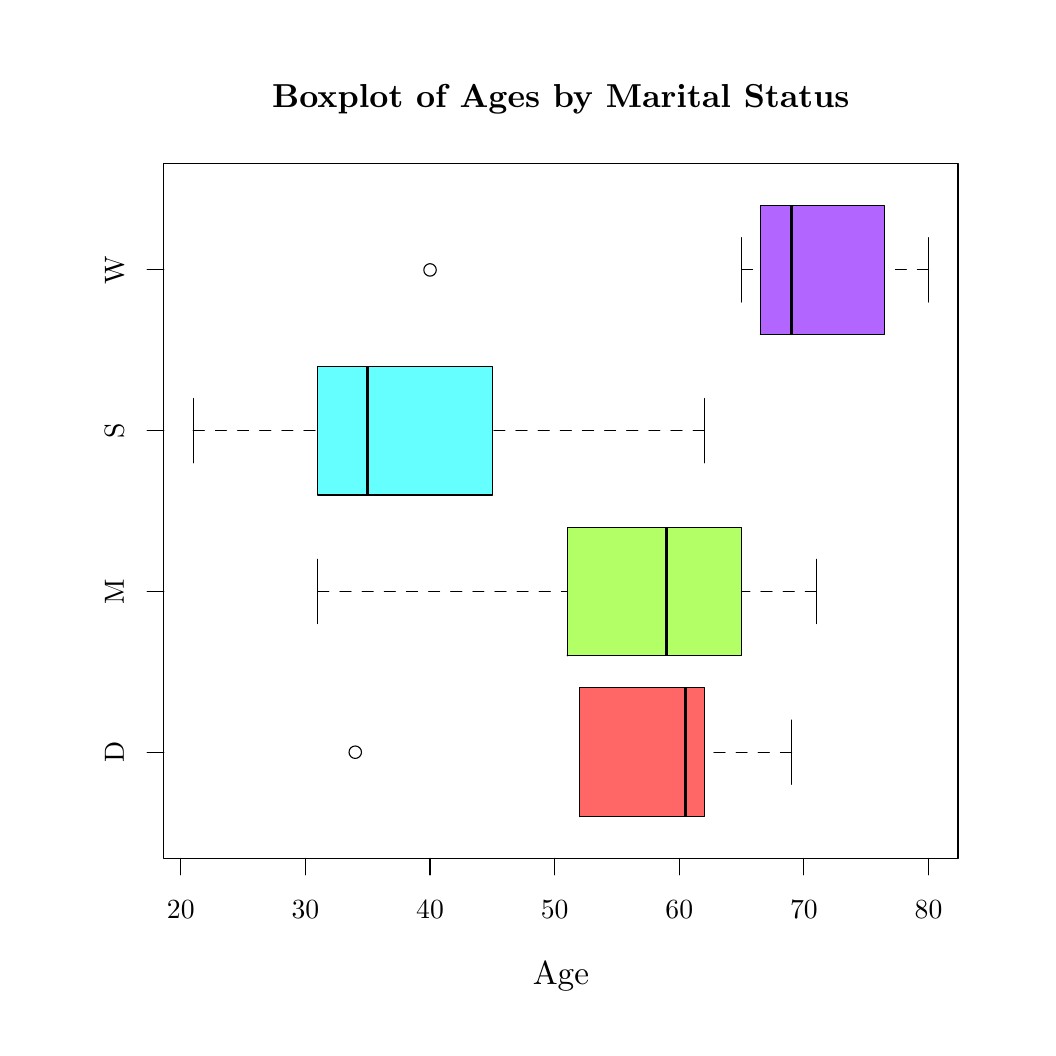
\begin{tikzpicture}[x=1pt,y=1pt]
\definecolor{fillColor}{RGB}{255,255,255}
\path[use as bounding box,fill=fillColor,fill opacity=0.00] (0,0) rectangle (361.35,361.35);
\begin{scope}
\path[clip] ( 49.20, 61.20) rectangle (336.15,312.15);
\definecolor{fillColor}{RGB}{255,102,102}

\path[fill=fillColor] (199.43, 76.30) --
	(199.43,122.78) --
	(244.46,122.78) --
	(244.46, 76.30) --
	cycle;
\definecolor{drawColor}{RGB}{0,0,0}

\path[draw=drawColor,line width= 1.2pt,line join=round] (237.71, 76.30) -- (237.71,122.78);

\path[draw=drawColor,line width= 0.4pt,dash pattern=on 4pt off 4pt ,line join=round,line cap=round] (199.43, 99.54) -- (199.43, 99.54);

\path[draw=drawColor,line width= 0.4pt,dash pattern=on 4pt off 4pt ,line join=round,line cap=round] (275.99, 99.54) -- (244.46, 99.54);

\path[draw=drawColor,line width= 0.4pt,line join=round,line cap=round] (199.43, 87.92) -- (199.43,111.16);

\path[draw=drawColor,line width= 0.4pt,line join=round,line cap=round] (275.99, 87.92) -- (275.99,111.16);

\path[draw=drawColor,line width= 0.4pt,line join=round,line cap=round] (199.43, 76.30) --
	(199.43,122.78) --
	(244.46,122.78) --
	(244.46, 76.30) --
	(199.43, 76.30);

\path[draw=drawColor,line width= 0.4pt,line join=round,line cap=round] (118.37, 99.54) circle (  2.25);
\definecolor{fillColor}{RGB}{179,255,102}

\path[fill=fillColor] (194.93,134.39) --
	(194.93,180.87) --
	(257.97,180.87) --
	(257.97,134.39) --
	cycle;

\path[draw=drawColor,line width= 1.2pt,line join=round] (230.95,134.39) -- (230.95,180.87);

\path[draw=drawColor,line width= 0.4pt,dash pattern=on 4pt off 4pt ,line join=round,line cap=round] (104.86,157.63) -- (194.93,157.63);

\path[draw=drawColor,line width= 0.4pt,dash pattern=on 4pt off 4pt ,line join=round,line cap=round] (284.99,157.63) -- (257.97,157.63);

\path[draw=drawColor,line width= 0.4pt,line join=round,line cap=round] (104.86,146.01) -- (104.86,169.25);

\path[draw=drawColor,line width= 0.4pt,line join=round,line cap=round] (284.99,146.01) -- (284.99,169.25);

\path[draw=drawColor,line width= 0.4pt,line join=round,line cap=round] (194.93,134.39) --
	(194.93,180.87) --
	(257.97,180.87) --
	(257.97,134.39) --
	(194.93,134.39);
\definecolor{fillColor}{RGB}{102,255,255}

\path[fill=fillColor] (104.86,192.48) --
	(104.86,238.96) --
	(167.91,238.96) --
	(167.91,192.48) --
	cycle;

\path[draw=drawColor,line width= 1.2pt,line join=round] (122.87,192.48) -- (122.87,238.96);

\path[draw=drawColor,line width= 0.4pt,dash pattern=on 4pt off 4pt ,line join=round,line cap=round] ( 59.83,215.72) -- (104.86,215.72);

\path[draw=drawColor,line width= 0.4pt,dash pattern=on 4pt off 4pt ,line join=round,line cap=round] (244.46,215.72) -- (167.91,215.72);

\path[draw=drawColor,line width= 0.4pt,line join=round,line cap=round] ( 59.83,204.10) -- ( 59.83,227.34);

\path[draw=drawColor,line width= 0.4pt,line join=round,line cap=round] (244.46,204.10) -- (244.46,227.34);

\path[draw=drawColor,line width= 0.4pt,line join=round,line cap=round] (104.86,192.48) --
	(104.86,238.96) --
	(167.91,238.96) --
	(167.91,192.48) --
	(104.86,192.48);
\definecolor{fillColor}{RGB}{179,102,255}

\path[fill=fillColor] (264.73,250.57) --
	(264.73,297.05) --
	(309.76,297.05) --
	(309.76,250.57) --
	cycle;

\path[draw=drawColor,line width= 1.2pt,line join=round] (275.99,250.57) -- (275.99,297.05);

\path[draw=drawColor,line width= 0.4pt,dash pattern=on 4pt off 4pt ,line join=round,line cap=round] (257.97,273.81) -- (264.73,273.81);

\path[draw=drawColor,line width= 0.4pt,dash pattern=on 4pt off 4pt ,line join=round,line cap=round] (325.52,273.81) -- (309.76,273.81);

\path[draw=drawColor,line width= 0.4pt,line join=round,line cap=round] (257.97,262.19) -- (257.97,285.43);

\path[draw=drawColor,line width= 0.4pt,line join=round,line cap=round] (325.52,262.19) -- (325.52,285.43);

\path[draw=drawColor,line width= 0.4pt,line join=round,line cap=round] (264.73,250.57) --
	(264.73,297.05) --
	(309.76,297.05) --
	(309.76,250.57) --
	(264.73,250.57);

\path[draw=drawColor,line width= 0.4pt,line join=round,line cap=round] (145.39,273.81) circle (  2.25);
\end{scope}
\begin{scope}
\path[clip] (  0.00,  0.00) rectangle (361.35,361.35);
\definecolor{drawColor}{RGB}{0,0,0}

\path[draw=drawColor,line width= 0.4pt,line join=round,line cap=round] ( 49.20, 99.54) -- ( 49.20,273.81);

\path[draw=drawColor,line width= 0.4pt,line join=round,line cap=round] ( 49.20, 99.54) -- ( 43.20, 99.54);

\path[draw=drawColor,line width= 0.4pt,line join=round,line cap=round] ( 49.20,157.63) -- ( 43.20,157.63);

\path[draw=drawColor,line width= 0.4pt,line join=round,line cap=round] ( 49.20,215.72) -- ( 43.20,215.72);

\path[draw=drawColor,line width= 0.4pt,line join=round,line cap=round] ( 49.20,273.81) -- ( 43.20,273.81);

\node[text=drawColor,rotate= 90.00,anchor=base,inner sep=0pt, outer sep=0pt, scale=  1.00] at ( 34.80, 99.54) {D};

\node[text=drawColor,rotate= 90.00,anchor=base,inner sep=0pt, outer sep=0pt, scale=  1.00] at ( 34.80,157.63) {M};

\node[text=drawColor,rotate= 90.00,anchor=base,inner sep=0pt, outer sep=0pt, scale=  1.00] at ( 34.80,215.72) {S};

\node[text=drawColor,rotate= 90.00,anchor=base,inner sep=0pt, outer sep=0pt, scale=  1.00] at ( 34.80,273.81) {W};

\path[draw=drawColor,line width= 0.4pt,line join=round,line cap=round] ( 55.32, 61.20) -- (325.52, 61.20);

\path[draw=drawColor,line width= 0.4pt,line join=round,line cap=round] ( 55.32, 61.20) -- ( 55.32, 55.20);

\path[draw=drawColor,line width= 0.4pt,line join=round,line cap=round] (100.36, 61.20) -- (100.36, 55.20);

\path[draw=drawColor,line width= 0.4pt,line join=round,line cap=round] (145.39, 61.20) -- (145.39, 55.20);

\path[draw=drawColor,line width= 0.4pt,line join=round,line cap=round] (190.42, 61.20) -- (190.42, 55.20);

\path[draw=drawColor,line width= 0.4pt,line join=round,line cap=round] (235.46, 61.20) -- (235.46, 55.20);

\path[draw=drawColor,line width= 0.4pt,line join=round,line cap=round] (280.49, 61.20) -- (280.49, 55.20);

\path[draw=drawColor,line width= 0.4pt,line join=round,line cap=round] (325.52, 61.20) -- (325.52, 55.20);

\node[text=drawColor,anchor=base,inner sep=0pt, outer sep=0pt, scale=  1.00] at ( 55.32, 39.60) {20};

\node[text=drawColor,anchor=base,inner sep=0pt, outer sep=0pt, scale=  1.00] at (100.36, 39.60) {30};

\node[text=drawColor,anchor=base,inner sep=0pt, outer sep=0pt, scale=  1.00] at (145.39, 39.60) {40};

\node[text=drawColor,anchor=base,inner sep=0pt, outer sep=0pt, scale=  1.00] at (190.42, 39.60) {50};

\node[text=drawColor,anchor=base,inner sep=0pt, outer sep=0pt, scale=  1.00] at (235.46, 39.60) {60};

\node[text=drawColor,anchor=base,inner sep=0pt, outer sep=0pt, scale=  1.00] at (280.49, 39.60) {70};

\node[text=drawColor,anchor=base,inner sep=0pt, outer sep=0pt, scale=  1.00] at (325.52, 39.60) {80};
\end{scope}
\begin{scope}
\path[clip] (  0.00,  0.00) rectangle (361.35,361.35);
\definecolor{drawColor}{RGB}{0,0,0}

\node[text=drawColor,anchor=base,inner sep=0pt, outer sep=0pt, scale=  1.20] at (192.68,332.61) {\bfseries Boxplot of Ages by Marital Status};

\node[text=drawColor,anchor=base,inner sep=0pt, outer sep=0pt, scale=  1.20] at (192.68, 15.60) {Age};
\end{scope}
\begin{scope}
\path[clip] (  0.00,  0.00) rectangle (361.35,361.35);
\definecolor{drawColor}{RGB}{0,0,0}

\path[draw=drawColor,line width= 0.4pt,line join=round,line cap=round] ( 49.20, 61.20) --
	(336.15, 61.20) --
	(336.15,312.15) --
	( 49.20,312.15) --
	( 49.20, 61.20);
\end{scope}
\end{tikzpicture}
}
\end{center}

\begin{enumerate}
\item Which group has higher ages?
\item Which group has lower central dispersion?
\item Which groups have outliers?
\item At which group is the age distribution more asymmetric?
\end{enumerate}
}
%SOLUTION
{
\begin{enumerate}
\item Widowers
\item Divorced.
\item Widowers and divorced.
\item Divorced.
\end{enumerate}
}
%RESOLUTION
{
}


\newproblem{des-60}{gen}{*}
%STATEMENT
{The systolic blood pressure (in mmHg) of a sample of persons is
\[
135\quad 128\quad 137\quad 110\quad 154\quad 142\quad 121\quad 127\quad 114\quad 103
\]

\begin{enumerate}
\item Calculate the central tendency statistics.
\item How is the relative dispersion with respect to the mean?
\item How is the skewness of the sample distribution?
\item How is the kurtosis of the sample distribution?
\item If we know that the method used for measuring the blood pressure is biased, and, in order to get the right values,
we have to apply the linear transformation $y=1.2x-5$, what are the statistics values of parts (a) to (d) for the new, corrected distribution?
\end{enumerate}


Use the following sums: $\sum x_i= 1271$ mmHg, $\sum (x_i-\bar x)^2=2188.9$ mmHg$^2$, $\sum (x_i-\bar x)^3=2764.32$
mmHg$^3$, $\sum (x_i-\bar x)^4=1040080$ mmHg$^4$.
}
%SOLUTION
{
Let $X$ be the systolic blood pressure.
\begin{enumerate}
\item $\bar{x}=127.1$ mmHg, $Me=127.5$ mmHg, $Mo=135$ mmHg.
\item $s=14.7949$ mmHg and $cv=0.1164$.
\item $g_1=0.0854$, so the distribution is almost symmetric.
\item $g_2=-0.8292$, so the distribution is flatter than a normal distribution (platykurtic).
\item $\bar{y}=147.52$ mmHg, $Me=148$ mmHg, $Mo=157$ mmHg, $s=17.7539$ mmHg, $cv=0.1203$, $g_1=0.0854$ and $g_2=-0.8292$.
\end{enumerate}
}
%RESOLUTION
{
}

\newproblem{des-61}{gen}{*}
%STATEMENT
{The table below contains the frequency of pregnancies, abortions and
births of a sample of 999 women in a city.

\begin{center}
\begin{tabular}{crrr}
\toprule
Num & Pregnancies & Abortions & Births\\
0 & 61 & 751 & 67 \\
1 & 64 & 183 & 80 \\
2 & 328 & 51 & 400 \\
3 & 301 & 10 & 300 \\
4 & 122 & 2 & 90 \\
5 & 81 & 2 & 62 \\
6 & 29 & 0 & 0 \\
7 & 11 & 0 & 0 \\
8 & 2 & 0 & 0 \\
\bottomrule
\end{tabular}
\end{center}

\begin{enumerate}
\item How many birth outliers are in the sample?
\item Which variable has lower spread with respect to the mean?
\item Which value is relatively higher, 7 pregnancies or 4 abortions? Justify your answer.
\end{enumerate}

Use the following sums:\\
Pregnancies: $\sum x_i= 2783$, $\sum x_i^2=9773$.\\
Abortions: $\sum x_i= 333$, $\sum x_i^2=559$.\\
Births: $\sum x_i= 2450$, $\sum x_i^2=7370$.
}
%SOLUTION
{
Let $X$ be the number of pregnancies, $y$ to the number of abortions and $z$ to the number of births.
\begin{enumerate}
\item 129 outliers.
\item Pregnancies: $\bar{x}=2.7858$, $s_x=1.422$ and $cv_x=0.5105$.\\
Abortions: $\bar{y}=0.3333$, $s_y=0.6697$ and $cv_y=2.009$.
Births: $\bar{z}=2.4525$, $s_z=1.1674$ and $cv_z=0.476$.
\item The standard score of 7 pregnancies is $2.9635$, y de standard score of 4 abortions is $5.4754$, so 4 abortions is relatively greater than 7 pregnancies.
\end{enumerate}
}
%RESOLUTION
{
}

% Author Alfredo Sánchez Alberca (asalber@ceu.es)

\section{Regression and correlation}
\begin{enumerate}[leftmargin=*,resume]
\item Give some examples of:
\begin{enumerate}
\item Non related variables.
\item Variables that are increasingly related.
\item Variables that are decreasingly related.
\end{enumerate}

\item In an study about the effect of different doses of a medicament, 2 patients got 2 mg and took 5 days to cure, 4
patients got 2 mg and took 6 days to cure, 2 patients got 3 mg ant took 3 days to cure, 4 patients got 3 mg and took 5
days to cure, 1 patient got 3 mg and took 6 days to cure, 5 patients got 4 mg and took 3 days to cure and 2 patients got
4 mg and took 5 days to cure. 
\begin{enumerate}
\item Construct the joint frequency table.
\item Get the marginal frequency distributions and compute the main statistics for every variable. 
\item Compute the covariance and interpret it. 
\end{enumerate}

\item The table below shows the two-dimensional frequency distribution of a sample of 80 persons in a study about the
relation between the blood cholesterol ($X$) in mg/dl and the high blood pressure ($Y$).
\[
\begin{array}{|c||c|c|c||c|}
\hline
X\setminus Y & [110,130) & [130,150) & [150,170) & n_x \\
\hline\hline
[170,190)   &           &     4     &           & 12\\
\hline
[190,210)   &    10     &    12     &     4     &   \\
\hline
[210,230)   &     7     &           &     8     &   \\
\hline
[230,250)   &     1     &           &           & 18\\
\hline\hline
n_y          &           &    30     &    24    &    \\
\hline
\end{array}
\]

\begin{enumerate}
\item Complete the table.
\item Construct the linear regression model of cholesterol on pressure. 
\item Use the linear model to calculate the expected cholesterol for a person with pressure 160 mmHg. 
\item According to the linear model, what is the expected pressure for a person with cholesterol 270 mg/dl?
\end{enumerate}

Use the following sums:
$\sum x=16960$ mg/dl, $\sum y=11160$ mmHg, $\sum x^2=3627200$ (mg/dl)$^2$, $\sum y^2=1576800$ mmHg$^2$ y
$\sum xy=2378800$ mg/dl$\cdot$mmHg.

\item A research study has been conducted to determine the loss of activity of a drug.
The table below shows the results of the experiment.

\begin{center}
\begin{tabular}{|l|r|r|r|r|r|}
\hline
Time (in years) & 1 & 2 & 3 & 4 & 5 \\ \hline
Activity (\%) & 96 & 84 & 70 & 58 & 52 \\ \hline
\end{tabular}
\end{center}

\begin{enumerate}
\item  Construct the linear regression model of activity on time.
\item  According to the linear model, when will the activity be 80\%? When will the drug have lost all activity?
\end{enumerate}

\item A basket team is testing a new stretching program to reduce the injuries during the league. 
The data below show the daily number of minutes doing stretching exercises and the number of injuries along the league. 
\begin{center}
\begin{tabular}{lrrrrrrrr}
\toprule
Stretching minutes & 0 & 30 & 10 & 15 & 5 & 25 & 35 & 40\\
Injuries & 4 & 1 & 2 & 2 & 3 & 1 & 0 & 1\\
\bottomrule
\end{tabular}
\end{center}
\begin{enumerate}
\item Construct the regression line of the number of injuries on the time of stretching. 
\item What is the reduction of injuries for every minute of stretching? 
\item How many minutes of stretching are require for having no injuries? Is reliable this prediction?
\end{enumerate}

Use the following sums ($X$=Number of minutes stretching, and $Y$=number of injuries):
$\sum x_i = 160$ min, $sum y_j=14$ injuries, $\sum x_i^2= 4700$ min$^2$, $\sum y_j^2=36$ injuries$^2$ and $\sum
x_iy_j=160$  min$cdot$injuries.

\item A dietary center is testing a new diet in sample of 12 persons. 
The data below are the number of days of diet and the weight lost (in Kg) until them for every person.  
\begin{center}
(33 , 3.9), (51 , 5.9), (30 , 3.2), (55 , 6.0), (38 , 4.9), (62 , 6.2),\\
(35 , 4.5), (60 , 6.1), (44 , 5.6), (69 , 6.2), (47 , 5.8), (40 , 5.3)
\end{center}
\begin{enumerate}
\item Draw the scatter plot. According to the point cloud, what type of regression model explains better the relation
between the weight lost and the days of diet?
\item Construct the linear regression model and the logarithmic regression model of the weight lost on the number of
days of diet.
\item Use the best model to predict the weight that will lose a person afte 100 days of diet. 
Is this prediction reliable?
\end{enumerate}


\end{enumerate}


% Author Alfredo Sánchez Alberca (asalber@ceu.es)

\section{Probability}
\begin{enumerate}[leftmargin=*,resume]
\item Construct the sample space of the following random experiments:
\begin{enumerate}
\item Pick a random person and measure the gender and whether she or he is smoker or not. 
\item Pick a random person and measure the blood type and whether she or he is smoker or not.
\item Pick a random person and measure the gender, the blood type and whether she or he is smoker or not.
\end{enumerate}

\item There are two boxes with balls of different colors. 
The first box contains 3 white balls and 2 black balls, and the second one contains 2 blue balls, 1 red ball and 1 green
ball. 
Construct the sample space of the following random experiments:
\begin{enumerate}
\item Pick a random ball from every box. 
\item Pick two random balls from every box.
\end{enumerate}

\item The Morgan's laws state that given two events $A$ and $B$ from the same sample space, $\overline{A\cup B}=\bar A
\cap \bar B$ and $\overline{A\cap B}=\bar A \cup \bar B$.
Proof both statements graphically using Venn diagrams.

\item Calculate the probability of the following events of the random experiment consisting in tossing 3 coins: 
\begin{enumerate}
\item Get exactly 1 heads. 
\item Get exactly 2 tails.
\item Get two or more heads.
\item Get some tails. 
\end{enumerate}

\item In a laboratory there are 4 flasks with sulfuric acid and 2 with nitric acid, and in another laboratory there are
1 flask with sulfuric acid and 3 with nitric acid. 
A random experiment consist in picking two flask, one from every laboratory. 
Calculate the probability of the following events:

\begin{enumerate}
\item The two picked flasks are of sulfuric acid.
\item The two picked flasks are of nitric acid.
\item The tow picked flasks contains different acids.
\end{enumerate}
Calculate the same probabilities if the flask picked in the first laboratory is put in the second laboratory before
picking the flask from it. 

\item Let $A$ and $B$ be events of the same sample space, such that $P(A)=3/8$, $P(B)=1/2$, $P(A\cap B)=1/4$.
Calculate the following probabilities:
\begin{enumerate}
\item  $P(A\cup B)$.
\item  $P(\bar A)$ y $P(\bar B)$.
\item  $P(\bar A\cap \bar B)$.
\item  $P(A\cap \bar B)$.
\item  $P(A|B)$.
\item  $P(A|\bar B)$.
\end{enumerate}

\item In a hospital the probability of getting hepatitis in a blood transfusion from a unit of blood is $0.01$.
A patient gets two units of blood while staying at the hospital.
What is the probability of getting hepatitis?

\item Let $A$ and $B$ be two events of the same sample space, such that $P(A)=0.6$ and $P(A\cup B)=0.9.$
Calculate $P(B)$ with the following assumptions:
\begin{enumerate}
\item $A$ and $B$ are incompatible.
\item $A$ and $B$ are independent.
\end{enumerate}

\item A study about smoking has published that 40\% of smokers have a smoker father, 25\% have a smoker mother and 52\%
have al least one of the parents smoker.
We pick a random person from this population.
Answer the following questions: 
\begin{enumerate}
\item What is the probability of having a smoker mother if the father smokes?
\item What is the probability of having a smoker mother if the father doesn't smoke?
\item Are independent the events having a smoker father and having a smoker mother?
\end{enumerate}

\item The probability that an injury $A$ is repeated is $4/5$, the probability that another injury $B$ is repeated is
$1/2$, and the probability that both injuries are repeated is $1/3$.
Calculate the probability of the following events:
\begin{enumerate}
\item Only injury $B$ is repeated.
\item At least one injury is repeated.
\item Injury $B$ is repeated if injury $A$ has been repeated.
\item Injury $B$ is repeated if injury $A$ hasn't been repeated. 
\end{enumerate}

\item In a digestive clinic from every 1000 patients that arrive with stomach pain, 700 have gastritis,
200 have an ulcer and 100 have cancer.
After analyzing the gastric symptoms, it is known that the probability of having vomiting is $0.3$ in case of gastritis,
$0.6$ in case of ulcer and $0.9$ in case of cancer. 
What is the diagnosis for a new patient with stomach pain that has vomiting?

Note: Assume that the only diseases are gastritis, ulcer and cancer and that are incompatible among them.  

\item To evaluate the effectiveness of a diagnosis test, the test was applied to a sample of 6900 people with the
following results:

\begin{center}
\begin{tabular}{|l|c|c|}
\cline{2-3}
\multicolumn{1}{l|}{} & Test $+$ & Test $-$ \\
\hline
Sick & 4680 & 120 \\
\hline
Healthy & 120 & 2020 \\
\hline
\end{tabular}
\end{center}

Calculate for this test:
\begin{enumerate}
\item The sensibility and the specificity.
\item The positive and negative predictive value.
\item The probability of a correct diagnosis. 
\end{enumerate}

\item We know, from a research study, that 10\% of people over 50 years suffer a particular type or arthritis.
We have developed a new method to detect the disease and after clinical trials we observe that if we apply the method to
people with arthritis we get a positive result in 85\% of cases, while if we apply the method to people without
arthritis, we get a positive result in 4\% of cases.
Answer the following questions:
\begin{enumerate}
\item What is the probability of getting a positive result after applying the method to a random person?
\item If the result of applying the method to one person has been positive, what is the probability of having arthritis?
\end{enumerate}

\item A severe pain without effusion in a particular zone of the knee joint is a symptom of sprained lateral collateral
ligament (SLCL). 
If the sprains in that ligament are classified into grade 1, when there is only distension (60\% of cases), grade 2 when
there is a partial tearing (30\% of cases) and grade 3 when there is a complete tearing (10\% of cases).
Taking into account that the symptom appears in 80\% of cases of grade 1 sprains, 90\% of cases of grade 2 and 100\% of
cases of grade 3, answer the following questions:

\begin{enumerate}
\item If a person has SLCL what is the probability that he or she present severe pain without effusion?
\item What is the diagnosis for a person with severe pain without effusion?
\item From a total of 10000 people with severe pain without effusion, how many are expected to have a grade 1 sprain? 
How many are expected to have a grade 2 sprain? And a grade 3 sprain?
\end{enumerate}


\end{enumerate}


% Author Alfredo Sánchez Alberca (asalber@ceu.es)

\newproblem{vad-1}{gen}{}
%STATEMENT
{Let $X$ be a discrete random variable with the following probability distribution
\[
\begin{array}{|c|c|c|c|c|c|}
\hline
X & 4 & 5 & 6 & 7 & 8 \\ 
\hline
f(x) & 0.15 & 0.35 & 0.10 & 0.25 & 0.15 \\ 
\hline
\end{array}
\]
\begin{enumerate}
\item  Compute and represent graphically the distribution function.
\item  Compute the following probabilities
\begin{enumerate}
\item  $P(X<7.5)$.
\item  $P(X>8)$.
\item  $P(4\leq X\leq 6.5)$.
\item  $P(5<X<6)$.
\end{enumerate}
\end{enumerate}
}
%SOLUTION
{
\begin{enumerate}
\item \[
F(x)=
\begin{cases}
0 & \text{if $x<4$,}\\
0.15 & \text{if $4\leq x<5$,}\\
0.5 & \text{if $5\leq x<6$,}\\
0.6 & \text{if $6\leq x<7$,}\\
0.85 & \text{if $7\leq x<8$,}\\
1 & \text{if $8\leq x$.}
\end{cases}
\]
\item $P(X<7.5)=0.85$, $P(X>8)=0$, $P(4\leq x\leq 6.5)=0.6$ and $P(5<X<6)=0$.
\end{enumerate}
}
%RESOLUTION
{}


\newproblem{vad-2}{gen}{}
%STATEMENT
{Let $X$ be a discrete random variable with the following probability distribution
\[
F(x)=
\begin{cases}
0 & \text{if $x<1$,} \\
1/5 & \text{if $1\leq x< 4$,} \\
3/4 & \text{if $4\leq x<6$,} \\
1 & \text{if $6\leq x$.}
\end{cases}
\]

\begin{enumerate}
\item  Compute the probability function.
\item  Compute the following probabilities
\begin{enumerate}
\item  $P(X=6)$.
\item  $P(X=5)$.
\item  $P(2<X<5.5)$.
\item  $P(0\leq X<4)$.
\end{enumerate}
\item Compute the mean. 
\item Compute the standard deviation. 
\end{enumerate}
}
%SOLUTION
{
\begin{enumerate}
\item \[
\begin{array}{|c|c|c|c|}
\hline
X & 1 & 4 & 6 \\
\hline
f(x) & 1/5 & 11/20 & 1/4\\
\hline
\end{array}
\]
\item $P(X=6)=1/4$, $P(X=5)=0$, $P(2<X<5.5)=11/20$ and $P(0\leq X<4)=1/5$.
\item $\mu=3.9$.
\item $\sigma=1.6703$.
\end{enumerate}
}
%RESOLUTION
{}


\newproblem{vad-3}{med}{*}
%STATEMENT
{An experiment consist in injecting a virus to three rats and checking if they survive or not. 
It is known that the probability of surviving is $0.5$ for the first rat, $0.4$ for the second and $0.3$
for the third.
\begin{enumerate}
\item Compute the probability function of the variable $X$ that measures the number of surviving rats.
\item Compute the distribution function.
\item Compute $P(X\leq 1)$, $P(X\geq 2)$ and $P(X=1.5)$.
\item Compute the mean and the standard deviation. 
Is representative the mean?
\end{enumerate}
}
%SOLUTION
{
\begin{enumerate}
\item \[
\begin{array}{|c|c|c|c|c|}
\hline
X & 0 & 1 & 2 & 3 \\
\hline
f(x) & 0.21 & 0.44 & 0.29 & 0.06\\
\hline
\end{array}
\]
\item \[
F(x)=
\begin{cases}
0 & \text{if $x<0$,}\\
0.21 & \text{if $0\leq x<1$,}\\
0.65 & \text{if $1\leq x<2$,}\\
0.94 & \text{if $2\leq x<3$,}\\
1 & \text{if $3\leq x$.}
\end{cases}
\]
\item $P(X\leq 1)=0.65$, $P(X\geq 2)=0.35$ y $P(X=1.5)=0$.
\item $\mu=1.2$ ratas, $\sigma^2=0.7$ ratas$^2$ y $\sigma=0.84$ ratas.
\end{enumerate}
}
%RESOLUTION
{}


\newproblem*{vad-4}{gen}{}
%STATEMENT
{Una tómbola asegura que en cada 1000 boletos hay 500 con ``siga intentándolo'', 100 con un premio de 1\euro, 60 con un premio de 2\euro, 30 con un premio de 3\euro, y 10 con un premio de 10\euro. Un individuo decide comprar un boleto que cuesta 1\euro. Se pide:

\begin{enumerate}
\item Construir una variable aleatoria que mida la ganancia (o pérdida) con la compra de un boleto.
\item ¿Cual es la probabilidad de que pierda dinero?
\item ¿Qué ganancia espera obtener?
\end{enumerate}
}
%SOLUTION
{}
%RESOLUTION
{}


\newproblem{vad-5}{med}{}
%STATEMENT
{The chance of being cured with certain treatment is $0.85$. 
If we apply the treatment to 6 patients,
\begin{enumerate}
\item What is the probability that half of them get cured?
\item What is the probability that a least 4 of them get cured?
\end{enumerate}
}
%SOLUTION
{Let $X$ be the number of cured patients in the sample of 6 treated patients, we have $X\sim B(6,0.85)$.
\begin{enumerate}
\item $P(X=3)=0.041$.
\item $P(X\geq 4)=0.9526$.
\end{enumerate}
}
%RESOLUTION
{}


\newproblem*{vad-6}{gen}{*}
%STATEMENT
{En una mesa de juego, en 1654, Meré propuso a Pascal la siguiente afirmación: ``es más probable obtener al menos un as con cuatro dados, que al menos un doble as en veinticuatro tiradas de dos dados''.

Demostrar que Meré tenía razón.
}
%SOLUTION
{}
%RESOLUTION
{}


\newproblem{vad-7}{med}{}
%STATEMENT
{It is known that the probability having a bacteria in one mm$^3$ of a dissolution is $0.002$.
Assuming that in one mm$^3$ can not be more than one bacteria, compute the probability of having 5 bacteria at most in one cm$^3$ of the dissolution.}
%SOLUTION
{Let $X$ be the number of bacteria in one cm$^3$ of dissolution, we have that $X\sim B(1000,0.002)\approx P(2)$.\\
$P(X\leq 5)=0.9834$.
}
%RESOLUTION
{}


\newproblem{vad-8}{med}{}
%STATEMENT
{Ten persons came into contact with a person infected with tuberculosis. 
The probability of being infected after contacting a person with tuberculosis is $0.10$.
\begin{enumerate}
\item What is the probability that nobody is infected?
\item What is the probability that at least 2 persons are infected?
\item What is the expected number of infected persons? 
\end{enumerate}
}
%SOLUTION
{Let $X$ be the number of persons infected with tuberculosis, we have $X\sim B(10,0.1)$. 
\begin{enumerate}
\item $P(X=0)=0.3487$. 
\item $P(X\geq 2)=0.2639$.
\item $\mu=1$.
\end{enumerate}
}
%RESOLUTION
{}


\newproblem*{vad-9}{gen}{*}
%STATEMENT
{Las matrículas de los coches constan de una parte numérica formada por cuatro cifras, y una parte literal. Se pide:

\begin{enumerate}
\item  Hallar la probabilidad de que al pasar 30 coches haya menos de dos cuya parte numérica sea capicúa.
\item  ¿Cuántos coches deben pasar para que la probabilidad de que alguno tenga la parte numérica capicúa sea mayor
que 0.1?
\end{enumerate}
}
%SOLUTION
{}
%RESOLUTION
{}


\newproblem{vad-10}{med}{}
%STATEMENT
{The probability of suffering an adverse reaction to a vaccine is $0.001$. 
If 2000 persons are vaccinated, what is the probability of suffering some adverse reaction?
}
%SOLUTION
{Let $X$ be the number of adverse reactions, we have that $X\sim B(2000,0.001)\approx P(2)$, and $P(X\geq 1)=0.8648$.
}
%RESOLUTION
{}


\newproblem{vad-11}{gen}{*}
%STATEMENT
{The average number of calls per minute received by a telephone switchboard is 120. 
\begin{enumerate}
\item What is the probability of receiving less than 4 calls in 2 seconds?
\item What is the probability of receiving at least 3 calls in 3 seconds?
\end{enumerate}
}
%SOLUTION
{
\begin{enumerate}
\item If $X$ is the number of calls in 2 seconds, then $X\sim P(4)$ and $P(X<4)=0.4335$.
\item If $Y$ is the number of calls in 3 seconds, then $Y\sim P(6)$ and $P(Y\geq 3)=0.938$.
\end{enumerate}
}
%RESOLUTION
{}


\newproblem*{vad-12}{nut}{}
%STATEMENT
{En un laboratorio de análisis de alimentos se sabe, de experiencias anteriores, que la probabilidad de que una muestra de café contenga plomo en cantidades superiores a las permitidas por la legislación vigente es $0.2$. Si se reciben $50$ muestras de café, ¿cuál es la probabilidad de rechazar al menos $5$?
¿Cuál será el número medio de muestras que rechazaremos?
}
%SOLUTION
{}
%RESOLUTION
{}


\newproblem{vad-13}{far}{}
%STATEMENT
{The fabrication process of a drug produces 6 defective units by hour on average.
What is the probability of producing less than 3 defective units in one hour?
And what is the probability of producing more than one defective units in half an hour?}
%SOLUTION
{Let $X$ be the number of defective units in one hour, we have that $X\sim P(6)$ and $P(X<3)=0.062$.\\
Let $Y$ be the number of defective units in half an hour, we have that $Y\sim P(3)$ and $P(Y>1)=0.8009$.}
%RESOLUTION
{}


\newproblem{vad-14}{gen}{}
%STATEMENT
{Una mecanógrafa comete, en promedio, una errata cada 2000 caracteres que escribe.
Suponiendo que escribe un folio con treinta líneas y setenta caracteres por línea, ¿cuál es la probabilidad de que
cometa más de un error en dicho folio?}
%SOLUTION
{Llamando $X$ al número de errores en un folio, se tiene que $X\sim B(2100,1/2000)\approx P(1.05)$, y $P(X>1)=0.2826$.
}
%RESOLUTION
{}


\newproblem{vad-15}{gen}{}
%STATEMENT
{A test contains 10 questions with 3 possible options each. 
For every question you get a point if you give the right answer and lose half a point if the answer is wrong. 
A student knows the right answer for 3 of the 10 questions and answers the rest randomly. 
What is the probability of passing the exam?}
%SOLUTION
{Let $X$ be the number of right questions in the 7 questions randomly answered, we have that $X\sim B(7,1/3)$ and $P(X\geq 4)=0.1733$.}
%RESOLUTION
{}


\newproblem*{vad-16}{gen}{*}
%STATEMENT
{Un equipo de fútbol tiene 7 delanteros. Se sabe que por término medio, cada delantero se pierde 5 partidos por lesión en una temporada de 40 partidos. Suponiendo que todos los delanteros tienen la misma probabilidad de lesionarse, se pide:
\begin{enumerate}
\item  ¿Cuál es la probabilidad de que en un partido determinado tenga menos de 5 delanteros en condiciones de jugar?
\item  ¿Cuál es la probabilidad de que a lo largo de la temporada haya más de un partido en que tenga menos de 5  delanteros en condiciones de jugar?
\end{enumerate}
}
%SOLUTION
{}
%RESOLUTION
{}


\newproblem*{vad-17}{amb}{}
%STATEMENT
{Para reforestar un bosque se compran árboles a un vivero en el que el 4\% de los árboles suele morir debido a una enfermedad. Si la repoblación se efectúa por parcelas en las que se ponen 10 árboles, se pide:
\begin{enumerate}
\item Calcular la probabilidad de que no muera ningún árbol en una parcela.
\item Calcular la probabilidad de no mueran más de 2 árboles en una parcela.
\item Si en total se reforestan 3000 parcelas, ¿cuál es la probabilidad de que haya alguna en la que mueran más de dos árboles?
\end{enumerate}
}
%SOLUTION
{}
%RESOLUTION
{}


\newproblem{vad-18}{med}{*}
%STATEMENT
{In a study about a parasite that attacks the kidney of rats it is known that the average number of parasites per
kidney is 3. 
\begin{enumerate}
\item Compute the probability that a rat has more than 3 parasites.
\item Compute the probability of, in a sample of 10 rats, at least 9 are infected. 
\end{enumerate}
}
%SOLUTION
{
\begin{enumerate}
\item If $X$ is the number of parasites in a rat, then $X\sim P(6)$ and $P(X>8)=0.1528$.
\item If $Y$ is the number of infected rats in a sample of 10 rats, then $Y\sim B(10,0.9975)$ and $P(Y\geq
9)=0.9997$.
\end{enumerate}
}
%RESOLUTION
{}


\newproblem{vad-19}{med}{*}
% ENUNCIADO
{It has been observed experimentally that 1 of every 20 trillions of cells exposed to radiation mutates becoming
carcinogenic. 
We know that the human body has approximately 1 trillion of cells by kilogram ot tissue. 
Compute the probability that a 60 kg person exposed to radiation develops cancer.
If the radiation affects 3 persons weighing 60 kg, what is the probability that a least one of them develops cancer? }
% SOLUCIÓN
{Let $X$ be the number of mutations, we have that $X\sim B(60\cdot 10^{12},1/20\cdot 10^{-12})\approx P(3)$ and $P(X>0)=0.9502$.\\ 
Let $Y$ be the number of persons that develops cancer in the group of 3 persons, we have that $Y\sim B(3,0.9502)$ and $P(Y\geq 1)=0.9999$.
}
% RESOLUCIÓN
{}


\newproblem{vad-20}{med}{*}
%STATEMENT
{En un servicio de urgencias de cierto hospital se sabe que, en media, llegan 2 pacientes a la hora.
Calcular:
\begin{enumerate}
\item Si los turnos en urgencias son de 8 horas, ¿cuál será la probabilidad de que en un turno lleguen más de 5 pacientes?
\item Si el servicio de urgencias tiene capacidad para atender adecuadamente como mucho a 4 pacientes a la hora, ¿cuál
es la probabilidad de que a lo largo de un turno de 8 horas el servicio de urgencias se vea desbordado en alguna de las
horas del turno?
\end{enumerate}
}
%SOLUTION
{
\begin{enumerate}
\item Llamando $X$ al número de pacientes en un turno, se tiene que $X\sim P(16)$ y $P(X>5)=0.9986$.
\item Llamando $Y$ al número de horas en el que el servicio se vea desbordado porque lleguen más de 4 pacientes, se
tiene que $Y\sim B(8,0.0527)$ y $P(Y\geq 1)=0.3515$.
\end{enumerate}
}
%RESOLUTION
{}


\newproblem*{vad-21}{amb}{}
%STATEMENT
{En un Parque Nacional se contabilizan 15 linces. Si sabemos, por estudios previos, que mueren en promedio 1 de cada 10 individuos a lo largo de un año (ya sea por accidentes, caza de furtivos o por causas naturales):
\begin{enumerate}
\item ¿Cuál es la probabilidad de que en el Parque Nacional se contabilicen más de 2 muertes de linces en un año?
\item Suponiendo un periodo de 12 años, ¿cuál es la probabilidad de que en el Parque Nacional haya algún año
en el que mueran 2 linces?
\end{enumerate}
}
%SOLUTION
{}
%RESOLUTION
{}


\newproblem{vad-22}{med}{*}
%STATEMENT
{The Turner syndrome is a genetic abnormality of women characterized by having only an $X$ chromosome.
It affects 1 in 2000 women approximately.
Besides, approximately 1 in 10 women with the Turner abnormality, also suffers a narrowing of the aorta.
\begin{enumerate}
\item In a sample of 4000 women, what is the probability of having more than 3 women with the Turner syndrome?
And what is the probability of having some women with a narrowing of the aorta as a consequence of the Turner syndrome?
\item In a sample of 20 women with the Turner syndrome, what is the probability of having less than 3 with a narrowing of the aorta?
\end{enumerate}
}
%SOLUTION
{
\begin{enumerate}
\item If $X$ is the number of women with the Turner syndrome in the sample of 4000 women, then $X\sim
B(4000,1/2000)\approx P(2)$ and $P(X>3)=0.1429$.\\
If $Y$ is the number of wome with a narrowing of the aorta in the sample of 4000 women, then $Y\sim
B(4000,1/20000)\approx P(0.2)$ and $P(Y>0)=0.1813$.
\item If $Z$ is the number of women with a narrowing of the aorta in the sample of 20 women with the Turner syndrome, then $Z\sim B(20,1/10)$ and $P(Z<3)=0.6769$.
\end{enumerate}
}
%RESOLUTION
{}


\newproblem{vad-23}{amb}{}
%STATEMENT
{Por estudios previos se sabe que, en una comarca, hay dos tipos de larvas que parasitan, de forma completamente
independiente, los chopos, y que producen su muerte.
Si la larva de tipo $A$ está parasitando un 15\% de los chopos, y la $B$ un 30\%, y en una zona concreta de la comarca
hay 10 chopos:
\begin{enumerate}
\item ¿Qué probabilidad hay que de estén siendo parasitados por $A$ más de dos?
\item ¿Qué probabilidad hay de que estén libres de $B$ más de 8?
\item ¿Qué probabilidad hay de que más de 1 tenga los dos tipos de larva?
\item ¿Qué probabilidad hay de que más de 3 tengan algún tipo de larva?
\end{enumerate}
}
%SOLUTION
{
\begin{enumerate}
\item $X_A$ es el número de chopos parasitados por larvas del tipo $A$, entonces $X_A\sim B(10,0.15)$ y
$P(X_A>2)=0.1798$.
\item Si $X_{\overline{B}}$ es el número de chopos no parasitados por larvas del tipo $B$, entonces
$X_{\overline{B}}\sim B(10,0.7)$ y $P(X_{\overline{B}}>8)=0.1493$.
\item Si llamamos $X_{A\cap B}$ al número de chopos parasitados por larvas de ambos tipos, entonces $X_{A\cap B}\sim
B(10,0.045)$ y $P(X_{A\cap B}>1)=0.0717$.
\item Si llamamos $X_{A\cup B}$ al número de chopos parasitados por algún tipo de larva, entonces $X_{A\cup B}\sim
B(10,0.405)$ y $P(X_{A\cup B}>3)=0.6302$.
\end{enumerate}
}
%RESOLUTION
{}


\newproblem*{vad-24}{amb}{*}
%STATEMENT
{En un Parque Regional se contabilizan 10 parejas de buitre leonado. Si sabemos que el 70\% de las parejas de esta especie logran que alguna de sus crías sobreviva:
\begin{enumerate}
\item ¿Cuál es la probabilidad de que 8 parejas de buitre leonado del Parque logren que alguna de sus crías sobreviva?
\item ¿Cuál es la probabilidad de que alguna pareja logre que alguna de sus crías sobreviva?
\item Si sabemos que en dicho Parque Regional nidifican, en promedio, 8 parejas al año, ¿cuál es la probabilidad de que en un año concreto nidifiquen más de 6?
\end{enumerate}
}
%SOLUTION
{}
%RESOLUTION
{}


\newproblem*{vad-25}{gen}{}
%STATEMENT
{Al lanzar 100 veces una moneda, ¿cuál es la probabilidad de obtener entre 40 y 60 caras?
}
%SOLUTION
{}
%RESOLUTION
{}


\newproblem{vad-26}{psi}{}
%STATEMENT
{El trastorno de pánico aparece en 1 de cada 75 personas.
¿Cuál es la probabilidad de que en un grupo de 100 personas aparezca alguna con trastorno de pánico?
¿Cuál es el número esperado de personas con trastorno de pánico en ese grupo?
}
%SOLUTION
{Llamando $X$ al número de personas que sufren trastorno del pánico en el grupo de 100 personas, se tiene que $X\sim
B(100,1/75)$ y $P(X\geq 1)=0.7379$.}
%RESOLUTION
{}


\newproblem{vad-27}{med}{}
%STATEMENT
{It is knwon that 2 in 1000 patients are allergic to drug $A$, and 6 in 1000 are allergic to drug $B$.
Besides, 30\% of patients allergic to drug $B$ are also allergic to drug $A$.
If we apply both drugs to a sample of 500 patients,
\begin{enumerate}
\item What is the probability of no patients being allergic to drug $A$?
\item What is the probability of at least 2 patients being allergic to drug $B$?
\item What is the probability of less than 2 patients being allergic to both drugs?
\item What is the probability of some patient being allergic to some of the drugs?
\end{enumerate}
}
%SOLUTION
{
\begin{enumerate}
\item Naming $X_A$ to the number of patients being allergic to drug $A$ in the sample of 500 patients, we have that $X_A\sim B(500,0.002)\approx P(1)$ and $P(X_A=0)=0.3678$.
\item Naming $X_B$ to the number of patients being allergic to drug $B$ in the sample of 500 patients, we have that $X_B\sim B(500,0.006)\approx P(3)$ and $P(X_B\geq 2)=0.8009$.
\item Naming $X_{A\cap B}$ to the number of patients being allergic to both drugs in the sample of 500 patients, we have that $X_A\sim B(500,0.0018)\approx P(0.9)$ and $P(X_{A\cap B}<2)=0.7725$.
\item Naming $X_{A\cup B}$ to the number of patients being allergic to some of the drugs in the sample of 500 patients, we have that $X_A\sim B(500,0.0062)\approx P(3.1)$ and $P(X_{A\cup B}\geq 1)=0.9550$.
\end{enumerate}
}
%RESOLUTION
{}


\newproblem{vad-28}{gen}{}
%STATEMENT
{In a classroom there are 40 students of which 35\% smoke.
If we draw a random sample with replacement of 4 students, what is the probability of having at least a smoker student?
Compute the same probability if the random sampling is without repalacement.}
%SOLUTION
{If $X$ is the number of smoker students in a random sample with replacement of size $4$, then $X\sim
B(4,0.35)$ and $P(X\geq 1)=0.8215$.\\
If the random sampling is without replacement then $P(X\geq 1)= 0.8364$.}
%RESOLUTION
{}


\newproblem{vad-29}{med}{*}
%STATEMENT
{Se sabe que por término medio 2 de cada 10000 niños que nacen son albinos.
\begin{enumerate}
\item Si en una región nacen cada año 22000 niños ¿cuál es la probabilidad de que un año nazcan al menos 4 albinos?
\item ¿Cuál es la probabilidad de que en esa región, en un periodo de 10 años no nazca ningún niño albino?
\end{enumerate}
}
%SOLUTION
{
\begin{enumerate}
\item Llamando $X$ al número de niños albinos que nacen en un año, se tiene que $X\sim B(22000,2/10000)\approx
P(4.4)$ y $P(X\geq 4)=0.6406$.
\item Llamando $Y$ al número de niños albinos que nacen en 10 años, se tiene que $Y\sim B(220000,2/10000)\approx
P(44)$ y $P(Y=0)=0$.
\end{enumerate}
}
%RESOLUTION
{}


\newproblem{vad-30}{med}{*}
%STATEMENT
{Suponiendo una facultad en la que hay un 60\% de chicas y un 40\% de chicos:
\begin{enumerate}
\item  Si un año van 6 alumnos a hacer prácticas en un hospital, ¿qué probabilidad hay de que vayan más chicos que chicas?
\item En un período de 5 años, ¿cuál es la probabilidad de que más de 1 año no haya ido ningún chico?
\end{enumerate}
}
%SOLUTION
{\begin{enumerate}
\item Si $X$ es el número de chicos, $X\sim B(6,0.4)$  y $P(X\geq 4)=0.1792$.
\item Si $Y$ es el número de años que no ha ido ningún chico, $Y \sim B(5,0.0467)$ y $P(Y>1)=0.0199$.
\end{enumerate}
}
%RESOLUTION
{\begin{enumerate}
\item Si consideramos un total de $n=6$ alumnos, con un $60\%$ de chicas y un $40\%$ de chicos, la variable $X$ que es el número de alumnos chicos que van a hacer las prácticas de un total de 6, sigue una distribución binomial de 6 intentos y probabilidad de éxito igual a $0.4$: $X\sim B(6,0.4)$. Como nos piden la probabilidad de que haya más chicos que chicas, eso se consigue si el número de chicos es 4 o más. Por lo tanto, nos piden la probabilidad de que $X$ sea mayor o igual que 4:
\[
P(X \ge 4) = P(X = 4) + P(X = 5) + P(X = 6)
\]
Calculando estas probabilidades con la función de probabilidad de la variable binomial, tenemos
\begin{align*}
P(X = 4) &= \binom{6}{4}\cdot 0.4^4  \cdot (1-0.4)^{6-4}  = 12\cdot 0.4^4\cdot 0.6^2 = 0.1382,\\
P(X = 5) &= \binom{6}{5}\cdot 0.4^5  \cdot (1-0.4)^{6-5}  = 6\cdot 0.4^5 \cdot 0.6 = 0.0369,\\
P(X = 6) &= \binom{6}{6}\cdot 0.4^6  \cdot (1-0.4)^{6-6}  = 1\cdot 0.4^6 \cdot 0.6^0 = 0.0041
\end{align*}
Y sumando los tres resultados obtenidos:
\[
P(X \ge 4) = P(X = 4) + P(X = 5) + P(X = 6)= 0.1382+0.0369+0.0041=0.1792.
\]

\item Si consideramos, en un total de 5 años, la probabilidad de que más de un año no haya ido ningún chico, la variable a tener en cuenta $Y$ será el número de años en el total de 5 sin ningún chico, y de nuevo esta variable sigue una distribución binomial, esta vez con 5 intentos, cuyo éxito viene dado por la probabilidad de que en un año concreto no haya ningún chico: $Y \sim B(5,p)$, donde $p=P(X=0)$.
\[
p = P(X = 0) = \binom{6}{0}\cdot 0.4^0  \cdot (1-0.4)^{6-0}  = 1\cdot 0.4^0\cdot 0.6^6 = 0.0467.
\]
Por lo tanto, $Y \sim B(5,0.0467)$.

Además, nos piden la probabilidad de más de una año en el total de 5; es decir: 
\[
P(Y>1)=1-P(Y\leq 1) = 1-P(Y=0)-P(Y=1).
\]
Aplicando, de nuevo, la fórmula de la función de probabilidad de la binomial, obtenemos:
\begin{align*}
P(Y = 0) &= \binom{5}{0}\cdot 0.0467^0  \cdot (1 - 0.0467)^{5-0} = 1\cdot 0.0467^0\cdot 0.9533^5  = 0.7873,\\
P(Y = 1) &= \binom{5}{1}\cdot 0.0467^1  \cdot (1 - 0.0467)^{5-1} = 5\cdot 0.0467^1\cdot 0.9533^4  = 0.1928.
\end{align*}
Teniendo lo anterior en cuenta, la probabilidad que nos piden vale:
\[
P(Y>1)=1-P(Y=0)-P(Y=1)=1-0.7873-0.1928=0.0199.
\]
\end{enumerate}
}


\newproblem*{vad-31}{med}{*}
%STATEMENT
{La probabilidad de que en un grupo de 5 individuos mayores de 70 años todos padezcan arterioesclerosis cerebral es de $12,5$ por mil.
\begin{enumerate}
\item ¿Cuál es la probabilidad de padecer la enfermedad entre los mayores de 70 años?
\item En un grupo de 1000 personas, ¿cuál es la probabilidad de que padezcan la enfermedad más de 450?
\end{enumerate}
}
%SOLUTION
{}
%RESOLUTION
{}


\newproblem{vad-32}{gen}{*}
%STATEMENT
{¿Cuánto habría que restar a cada pregunta errada en un examen de tipo test de 5 preguntas con cuatro opciones y sólo
una correcta, para que un individuo que responda al azar tenga una puntuación esperada de 0? 
}
%SOLUTION
{$1/3$.}
%RESOLUTION
{Si llamamos $X$ al número de preguntas acertadas, está claro que $X$ sigue una distribución binomial $B(5,1/4)$ ya
que el examen tiene 4 preguntas, y la probabilidad de acertar cualquiera de ellas al azar es $1/4$ ya que hay cuatro
opciones y sólo una es la correcta.
}


\newproblem{vad-33}{psi}{}
%STATEMENT
{Se sabe que el $6.8$\% las personas presentan a lo largo de su adolescencia un trastorno de hiperactividad, de los
cuales tres cuartas partes son mujeres.
Si en la población hay el mismo número de hombres y mujeres, se pide:
\begin{enumerate}
\item Calcular la probabilidad de que en una muestra de tres hombres, haya alguno que haya tenido hiperactividad en su
adolescencia. 
\item Calcular la probabilidad de que en una muestra de 2 hombres y 2 mujeres, haya alguno que haya tenido
hiperactividad en su adolescencia. 
\end{enumerate}
}
%SOLUTION
{
\begin{enumerate}
\item Si llamamos $X$ al número de hombres que han tenido hiperactividad en su adolescencia en una muestra de 3
hombres, se tiene que $X\sim B(3,0.034)$ y $P(X\geq 1)=0.0986$.
\item Si llamamos $X_H$ al número de hombres que han tenido hiperactividad en su adolescencia en una muestra de 2
hombres y $X_M$ al número de mujeres que han tenido hiperactividad en su adolescencia en una muestra de 2 mujeres,
entonces $X_H\sim B(2,0.034)$ y $X_M(2,0.102)$. Entonces $P(X_H\geq 1\cup X_M\geq 1)=0.2475$.
\end{enumerate}
}
%RESOLUTION
{}


\newproblem{vad-34}{gen}{*}
%STATEMENT
{A un hospital llegan pacientes por la mañana a efectuarse extracciones de sangre. Se ha medido la frecuencia de llegada de los mismos en
intervalos de 15 minutos. La distribución de probabilidad (medida de forma frecuentista) se  muestra en la siguiente tabla:
\[
\begin{array}{c|c|c|c|c|c|c|c|}
  X   &  0  &  1  &  2   &  3   &  4   &  5  &  6   \\
\hline
 P(x) & 0.1 & 0.2 & 0.25 & 0.15 & 0.15 & 0.1 & 0.05 \\
\end{array}
\]
Se pide:
\begin{enumerate}
\item Calcular la probabilidad de que en un intervalo de 15 minutos lleguen 2 o más personas, y probabilidad de que lleguen menos de 8
personas.
\item ¿Cuál es el número medio esperado de personas que llegarán a sacarse sangre cada 15 minutos?
\item Suponiendo que el número de personas que llegan a sacarse sangre en 15 minutos sigue una distribución de Poisson de media la  
calculada en el apartado anterior, ¿cuál es la probabilidad de que llegue alguna en 15 minutos? ¿Y de que llegue alguna en 5 minutos? 
\end{enumerate}
} 
%SOLUTION
{Llamemos $J$ al suceso consitente en que una persona con la lesión sea joven, $C$ al suceso consistente en curarse, y $A$ y $B$ a los sucesos consistentes en aplicar las respectivas técnicas de
rehabilitación:
\begin{enumerate}
\item Llamando $X$ al número de personas que llegan en un intervalo de 15 minutos: $P(X\geq 2)=0.7$ y $P(X<8)=1$.
\item $\mu=2.55$ personas.
\item Suponiendo $X\sim P(2.55)$, $P(X\geq 1)=0.9219$.\\
Llamando $Y$ al número de personas que llegan en un intervalo de 5 minutos, $P(Y\geq 1)=0.5726$.
\end{enumerate}
}
%RESOLUTION
{\begin{enumerate}
\item Teniendo en cuenta que nos dan la distribución de probabilidad de la variable aleatoria discreta $X$ que expresa el número de
pacientes que llegan en 15 minutos, nos están pidiendo $P(X\geq 2)$ y $P(X<8)$. Estas probabilidades son:
\begin{align*}
P(X\geq 2) & =1-P(X<2)=1-P(X=0)-P(X=1)=1-0.2-0.3=0.7,\\
P(X<8)& =1-P(X\geq 8)=1.
\end{align*}
\item El número esperado es la media de la variable aleatoria:
\[
\mu =\sum xf(x)=0\cdot 0.1+1\cdot 0.2+2\cdot 0.25+3\cdot 0.15+4\cdot 0.15+5\cdot 0.1+6\cdot 0.05=2.55 \text{ personas}.
\]

\item Suponiendo que $X$ sigue una distribución de Poisson con $\lambda =2.55$, $X\sim P(2.55),$ la probabilidad de que llegue alguna
persona en 15 minutos vendrá dada por:
\[
P(X\geq 1)=1-P(X=0)=1-e^{-2.55}\dfrac{2.55^{0}}{0!}=0.9219.
\]

Para la segunda pregunta, teniendo en cuenta que el número medio de personas que llegan cada 15 minutos es $2.55$, en 5 minutos llegarán en
media $2.55/3 = 0.85$ personas, y, por tanto, tenemos una nueva variable aleatoria $Y$, que seguirá una distribución de Poisson con $\lambda
^{\prime }=0.85.$
\[
P(Y\geq 1)=1-P(Y=0)=1-e^{-0.85}\dfrac{0.85^{0}}{0!}=0.5726.
\]
\end{enumerate}
}


\newproblem{vad-35}{gen}{*}
%STATEMENT
{En las siguientes tablas, indicar razonadamente, en los caso que sea posible,
los valores de $h$ que deben ponerse en cada tabla para que se tenga una
distribución de probabilidad:
\[
\begin{array}{c|c}
x & f(x) \\
\hline
-2 & 0.3  \\
5 & h  \\
8 & 0.1
\end{array}
\qquad
\begin{array}{c|c}
x & f(x) \\
\hline
 1 & -0.2 \\
 3 & 0.7 \\
 4 & h
\end{array}
 \qquad
\begin{array}{c|c}
x & f(x) \\
\hline
 2 & h \\
 3 & 0.5 \\
 4 & 0.6
\end{array}
\]

En las tablas que constituyan una distribución de probabilidad:
\begin{enumerate}
\item Representar gráficamente la función de distribución.
\item Calcular media y desviación típica.
\item Calcular la mediana.
\item Si a los valores de $x$ se multiplican por una constante $k<0$, ¿cómo se ve afectada la media? ¿Y la desviación típica?
\end{enumerate}
} 
%SOLUTION
{La única tabla que puede ser una distribución de probabilidad es la primera para $h=0.6$.
\begin{enumerate}[start=2]
\item $\mu=3.2$ y $\sigma=3.516$.
\item $Me=5$.
\item $\mu_y=k\mu_x$ y $\sigma_y=|k|\sigma_x$.
\end{enumerate}
}
%RESOLUTION
{La segunda tabla no puede ser una distribución de probabilidad pues $f(1)=-0.2$ y la función de probabilidad no puede tomar valores
negativos. Por otro lado, la tercera tabla tampoco puede ser una distribución de probabilidad ya que la suma de todas las probabilidades
debe ser 1, y para ello debería ser $h=-0.1$, lo cual no es posible al no poder tomar valores negativos. Así pues la única tabla que puede
ser una distribución de probabilidad es la primera, y como la suma de todas las probabilidades tiene que ser 1, $0.3+h+0.1=1$, se deduce que
$h=0.6$. Trabajaremos pues, con la distribución
\[
\begin{array}{r|r}
 x  & f(x) \\
\hline
 -2 & 0.3  \\
 5  & 0.6  \\
 8  & 0.1  \\
\end{array}
\]

\begin{enumerate}
\item La función de distribución se define como $F(x_0)=P(X\leq x_0)$, y por tanto,  mide probabilidades acumuladas. Acumulando las
probabilidades de la tabla anterior tenemos
\[
\begin{array}{r|r|r}
 x  & \multicolumn{1}{c|}{f(x)} & \multicolumn{1}{c}{F(x)}\\
\hline
 -2 & 0.3 & 0.3 \\
 5  & 0.6 & 0.9 \\
 8  & 0.1 & 1 \\
\end{array}
\]
O lo que es lo mismo, expresado como una función a trozos
\[
F(x)=
\left\{%
\begin{array}{ll}
   0, & \hbox{si $x<-2$;} \\
   0.3, & \hbox{si $-2\leq x<5$;} \\
   0.9, & \hbox{si $5\leq x<8$;} \\
   1, & \hbox{si $x\geq 8$.} \\
\end{array}%
\right.
\]

La gráfica de esta función es la siguiente
\begin{center}
\includegraphics[scale=0.3]{grafica1}\hspace*{1cm}
\end{center}

\item Calculamos los estadísticos que nos piden
\begin{align*}
\mu &= \sum x_if(x_i)=-2\cdot0.3+5\cdot 0.6+8\cdot 0.1=3.2,\\
\sigma^2 &= \sum x_i^2f(x_i)-\mu^2=(-2)^2\cdot 0.3+5^2\cdot 0.6+8^2\cdot 0.1-3.2^2=22.6-10.24=12.36,\\
\sigma &= \sqrt{12.36}=3.516.
\end{align*}

\item La mediana es el valor que deja acumulada una probabilidad $0.5$, es decir, $F(med)=0.5$, y mirando en la función de distribución, el
valor donde se consigue acumular esta probabilidad es el 5.

\item Sea $Y=kX$ donde $k<0$. Por las propiedades de las transformaciones lineales de variables aleatorias, tenemos que $\mu_y=k\mu_x$, y
por tanto la media quedará también multiplicada por la constante $k$. Para la desviación típica tenemos que $\sigma_y=|k|\sigma_x$ y la
desviación típica quedará multiplicada por el valor absoluto de $k$.
\end{enumerate}
}


\newproblem{vad-36}{gen}{*}
%STATEMENT
{En una empresa el número de días al año que los empleados están de baja es, por término medio, 5. Suponiendo que un año tiene 240 días
laborables y que cada mes tiene 20, se pide:
\begin{enumerate}
\item Calcular el porcentaje de empleados que no faltarían más de 5 días al año.
\item Calcular la probabilidad de que un empleado falte algún día en un mes.
\item ¿Cual es la probabilidad de que en un año haya más de 2 meses en los que haya faltado alguna vez?
\end{enumerate}
} 
%SOLUTION
{
\begin{enumerate}
\item Llamando $X$ a la variable que mide el número de días de baja al año de cada empleado, $X\sim B(240,5/240)\approx P(5)$ y
$P(X\leq 5)=0.616$.
\item Llamando $Y$ a la variable que mide el número de días de baja al mes de cada empleado, $Y\sim B(20,5/240)$ y $P(Y\geq 1)=0.3437$.
\item Llamando $Z$ a la variable que mide el número de meses al año en que un empleado falta alguna vez, $Z\sim B(12,0.3437)$ y
$P(Z>2)=0.8379$.
\end{enumerate}
}
%RESOLUTION
{
\begin{enumerate}
\item Sea $X$ la variable que mide el número de días de baja al año de cada empleado. Entonces \mbox{$X\sim B(240,5/240)$}, pero como
$n=240>30$ y $p=5/240<0.1$, podemos aproximarla como una distribución Poisson $P(5)$. La probabilidad de que un empleado no falte más de 5
días al año es
\begin{align*}
P(X\leq 5)&= P(X=0)+P(X=1)+P(X=2)+P(X=3)+P(X=4)+P(X=5)= \\
&= e^{-5}\frac{5^0}{0!}+
e^{-5}\frac{5^1}{1!}+e^{-5}\frac{5^2}{2!}+e^{-5}\frac{5^3}{3!}
+e^{-5}\frac{5^4}{4!}+e^{-5}\frac{5^5}{5!}= \\
&= 0.0067+0.0337+0.0842+0.1404+0.1755+0.1755=0.616,
\end{align*}
es decir, un $61.6\%$.

\item Sea $Y$ la variable que mide el número de días de baja al mes de cada empleado. Entonces \mbox{$Y\sim B(20,5/240)$}, y la
probabilidad de que algún empleado falte algún día en un mes es
\begin{align*}
P(Y\geq1)&=1-P(Y<1)=1-P(Y=0)=
1-\binom{20}{0}\left(\frac{5}{240}\right)^0\left(1-\frac{5}{240}\right)^{20}= \\
&=1-\left(\frac{235}{240}\right)^{20}=0.3437.
\end{align*}

\item Sea ahora $Z$ la variable que mide el número de meses al año en que un empleado falta alguna vez. Entonces, como la probabilidad de
que un empleado falte alguna vez en un mes, según el apartado anterior es $0.3437$, tenemos que $Z\sim B(12,0.3437)$. Así pues, la
probabilidad que nos piden  es
\begin{align*}
P(Z>2)&=1-P(Z\leq 2)=1-P(Z=0)-P(Z=1)-P(Z=2)=\\
&= 1-\binom{12}{0}0.3437^0 0.6563^{12}-\binom{12}{1}0.3437^1 0.6563^{11}-
\binom{12}{2}0.3437^2 0.6563^{10}=\\
&=1-0,0064-0,0401-0,1156=0.8379.
\end{align*}
\end{enumerate}
}


\newproblem{vad-37}{med}{*}
%STATEMENT
{Sabiendo que la prevalencia de la isquemia cardíaca es del 1\%, y que la aplicación de un test diagnóstico para detectar la isquemia
cardíaca tiene una sensibilidad del 90\%, y una especificidad del 95\%. Calcular:
\begin{enumerate}
\item Los valores predictivos, tanto el positivo como el negativo.
\item La probabilidad de diagnóstico acertado.
\item Si tenemos un grupo de 10 enfermos de isquemia cardíaca, ¿cuál es la probabilidad de que diagnostiquemos la enfermedad a
menos de 8?
\end{enumerate}
} 
%SOLUTION
{
}
%RESOLUTION
{
}


\newproblem{vad-38}{med}{*}
%STATEMENT
{A diagnostic test for a disease returns 1\% of positive outcomes, and the positivie and negative predictive values are $0.95$ and $0.98$ respectively. 
\begin{enumerate}
\item Compute the prevalence of the disease.
\item Compute the sensitivity and the specificity of the test.
\item If the test is applied to 12 sick persons, what is the probability of getting at least a wrong diagnostic?
\item If the test is applied to 12 persons, what is the probability of getting a right diagnostic for all of them?
\end{enumerate}
} 
%SOLUTION
{
\begin{enumerate}
\item $P(D)=0.0293$.
\item Sensitivity $P(+|D)=0.3242$ and specificity $P(-|\overline D)=0.9995$. 
\item Let $X$ be the number of wrong diagnostics in 12 sick individuals, we have that $x\sim B(12,0.6758)$ and $P(X\geq 1)=1$. 
\item Let $Y$ be the number of right diagnostics in 12 individuals, we we have that $Y\sim B(12,0.9797)$ and $P(Y=12)=0.7818$. 
\end{enumerate}
}
%RESOLUTION
{
}


\newproblem{vad-39}{med}{*}
%STATEMENT
{La probabilidad de que en un grupo de 5 individuos mayores de 70 años todos padezcan arterioesclerosis cerebral es de $12.5$ por mil.
\begin{enumerate}
\item ¿Cuál es la probabilidad de padecer la enfermedad entre los mayores de 70 años?
\item En un grupo de 1000 personas, ¿cuál es la probabilidad de que padezcan la enfermedad más de 450?
\end{enumerate}
} 
%SOLUTION
{
}
%RESOLUTION
{
}


\newproblem{vad-40}{med}{*}
%STATEMENT
{Si sabemos, por estudios previos, que las cepas que provocarán la gripe del siguiente otoño-invierno afectarán a un 20\% de la
población:
\begin{enumerate}
\item ¿Cuál es la probabilidad de que en una población de 10000 habitantes queden infectados menos de 1900?
\item Suponiendo que se vacunan los 10000 habitantes y sabiendo, por estudios previos, que la vacuna inmuniza al 98\% de los vacunados,
¿Cuál es la probabilidad de que queden sin inmunizar menos de 180?
\item De nuevo, suponiendo que se han vacunado los 10000 habitantes y teniendo en cuenta que, por estudios previos, la vacuna produce
reacciones alérgicas en uno de cada 5000 casos, ¿cuál es la probabilidad de que se produzca alguna reacción alérgica en dicha población?
\end{enumerate}
} 
%SOLUTION
{
}
%RESOLUTION
{
}


\end{document}
